% !TeX program = xelatex
% English edition of the thesis -- requires XeLaTeX (fontspec/polyglossia).
% Build: xelatex thesis_en.tex  x3  (from inside docs/)
% NOTE: delete thesis_en.aux/.toc/.out before each build (see CLAUDE.md).
\documentclass[12pt,a4paper,oneside]{report}

\usepackage{fontspec}
\usepackage{polyglossia}
\setmainlanguage{english}
\setotherlanguage{greek}
\setmainfont{Linux Libertine O}
\setsansfont{Linux Biolinum O}
\setmonofont{DejaVu Sans Mono}[Scale=0.85]

\usepackage[a4paper,margin=2.8cm]{geometry}
\usepackage{amsmath,amssymb,amsthm}
\usepackage{booktabs}
\usepackage{array}
\usepackage{float}
\usepackage{graphicx}
\graphicspath{{../results/}{./}}
\usepackage{enumitem}
\usepackage{caption}
\usepackage{xcolor}
\usepackage{longtable}
\usepackage[hidelinks]{hyperref}

\newcommand{\file}[1]{\texttt{#1}}
% kept as identity so any leftover \en{} from the Greek edition is harmless
\newcommand{\en}[1]{#1}
\let\oldunderscore\_
\renewcommand{\_}{\oldunderscore\allowbreak}
\setlength{\emergencystretch}{3em}
\setlist[itemize]{topsep=4pt,itemsep=3pt}
% the reference theses of this group head the list "References", not "Bibliography"
\addto\captionsenglish{\renewcommand{\bibname}{References}}

\theoremstyle{definition}
\newtheorem{definition}{Definition}[chapter]
\theoremstyle{plain}
\newtheorem{theorem}{Theorem}[chapter]
\newtheorem{lemma}[theorem]{Lemma}
\newtheorem{proposition}[theorem]{Proposition}
\newtheorem{corollary}[theorem]{Corollary}
\theoremstyle{remark}
\newtheorem{remark}[theorem]{Remark}

\begin{document}

% =====================================================================
% Title page
% =====================================================================
\begin{titlepage}
\centering

\vspace*{0.5cm}

\includegraphics[height=3.4cm]{tuc_logo.png}\par

\vspace{0.8cm}

{\large TECHNICAL UNIVERSITY OF CRETE\par}
\vspace{0.35em}
{\normalsize SCHOOL OF ELECTRICAL AND COMPUTER ENGINEERING\par}
\vspace{0.35em}
{\normalsize TELECOMMUNICATIONS DIVISION\par}

\vspace{1.8cm}

{\LARGE\bfseries Online Convex Optimization based tuning\\[0.4em]
of Mixture of Experts\\[0.4em]
for Sports Outcome Prediction\par}

\vspace{1.2cm}
{\large DIPLOMA THESIS\par}
\vspace{0.9cm}
{\Large\bfseries Stefanos Mousadis\par}

\vspace{1.5cm}

{\large THESIS COMMITTEE\par}
\vspace{0.7em}
{\normalsize
Prof. Thrasyvoulos Spyropoulos, \emph{Supervisor}\\[0.4em]
Prof. Michail G. Lagoudakis\\[0.4em]
Prof. Vasileios Samoladas\par}

\vspace{1.0cm}
{\small A thesis submitted in partial fulfilment of the requirements\\
for the Diploma Degree in Electrical and Computer Engineering\par}

\vspace{1.0cm}
{\large Chania, 2026\par}
\end{titlepage}

% ---------------------------------------------------------------------
% Greek title page, as in the reference theses of this group
% ---------------------------------------------------------------------
\begin{titlepage}
\centering
\begin{greek}

\vspace*{0.5cm}

\includegraphics[height=3.4cm]{tuc_logo.png}\par

\vspace{0.8cm}

{\large ΠΟΛΥΤΕΧΝΕΙΟ ΚΡΗΤΗΣ\par}
\vspace{0.35em}
{\normalsize ΣΧΟΛΗ ΗΛΕΚΤΡΟΛΟΓΩΝ ΜΗΧΑΝΙΚΩΝ ΚΑΙ ΜΗΧΑΝΙΚΩΝ ΥΠΟΛΟΓΙΣΤΩΝ\par}
\vspace{0.35em}
{\normalsize ΤΟΜΕΑΣ ΤΗΛΕΠΙΚΟΙΝΩΝΙΩΝ\par}

\vspace{2.4cm}

{\Large\bfseries Κυρτή Βελτιστοποίηση σε Πραγματικό Χρόνο\\[0.5em]
Βασισμένη στην Παραμετροποίηση Μείγματος Ειδικών\\[0.5em]
για την Πρόβλεψη Αποτελεσμάτων Αθλητικών Αγώνων\par}

\vspace{1.5cm}
{\large ΔΙΠΛΩΜΑΤΙΚΗ ΕΡΓΑΣΙΑ\par}
\vspace{1.1cm}
{\Large\bfseries Στέφανος Μουσάδης\par}

\vspace{2.0cm}

{\large ΕΞΕΤΑΣΤΙΚΗ ΕΠΙΤΡΟΠΗ\par}
\vspace{0.7em}
{\normalsize
Καθ. Θρασύβουλος Σπυρόπουλος, \emph{Επιβλέπων}\\[0.4em]
Καθ. Μιχαήλ Γ. Λαγουδάκης\\[0.4em]
Καθ. Βασίλειος Σαμολαδάς\par}

\vfill
{\large Χανιά, 2026\par}
\end{greek}
\end{titlepage}

\cleardoublepage

% =====================================================================
% Abstracts
% =====================================================================
\chapter*{Abstract}
\addcontentsline{toc}{chapter}{Abstract}

This thesis predicts sports match outcomes (home / draw / away) as a problem of
\textbf{online learning with expert advice}, rather than as the training of a statistical
model. Each betting operator is treated as an expert quoting odds on the three outcomes,
from which probabilities are derived. The task is to find a weight vector such that the
mixture of experts outperforms each of them individually, learning not retrospectively over
the past but match by match.

Three stages of \textbf{Online Convex Optimization} (OCO) are implemented. First, three
algorithms are built (Hedge, Online Gradient Descent, Follow-The-Regularized-Leader), which
handle partially covering operators through the \textbf{Sleeping Experts} reduction. A second
OCO stage then calibrates the mixture via online temperature scaling. Finally the bet size is
computed with the Kelly criterion, whose multiplier is itself learned online with Online
Newton Step. Every comparison is tested with a moving block bootstrap. The dataset spans
22 leagues, 10 seasons and 76,584 matches.

The mixture significantly outperforms every individual bookmaker except the sharpest, with
which it draws level in the configuration ultimately adopted. Under a deployment test with a
genuine temporal cut (fitted through the end of 2024, evaluated on 2025--26) it significantly
outperforms every opening price and draws level with the bookmakers' closing prices. The one
series that significantly outperforms it is Betfair Exchange, which is not a bookmaker but an
exchange, that is a market price carrying no operator's margin.

The three broader findings are that learning pays only where experts are heterogeneous in
quality; that better prediction does not translate directly into profit, since the quality
gain falls short of the market's margin; and that part of the advantage over the uniform
average is due not to learning but to the geometry of the Sleeping Experts reduction.

\vspace{1em}
\noindent\textbf{Keywords:} online convex optimization, prediction with expert advice,
sleeping experts, regret, probability calibration, betting markets

\cleardoublepage

\begin{greek}
\chapter*{Περίληψη}
\addcontentsline{toc}{chapter}{Περίληψη}

Η παρούσα εργασία προβλέπει τα αποτελέσματα αθλητικών αγώνων (1/Χ/2) ως πρόβλημα
\textbf{online μάθησης με συμβουλή ειδικών}, και όχι ως εκπαίδευση στατιστικού μοντέλου.
Κάθε στοιχηματικός πάροχος θεωρείται ένας expert που δίνει αποδόσεις για τα τρία ενδεχόμενα,
από τις οποίες προκύπτουν πιθανότητες. Ζητούμενο είναι η εύρεση ενός διανύσματος βαρών έτσι
ώστε το μείγμα των experts να τους ξεπερνά ατομικά, με μάθηση όχι αναδρομικά πάνω στο
παρελθόν, αλλά αγώνα προς αγώνα.

Υλοποιούνται τρία στάδια Κυρτής Βελτιστοποίησης σε Πραγματικό Χρόνο (\textbf{Online Convex
Optimization}, OCO). Αρχικά κατασκευάζονται τρεις αλγόριθμοι (Hedge, Online Gradient Descent,
Follow-The-Regularized-Leader), που με την αναγωγή σε \textbf{Sleeping Experts} διαχειρίζονται
τους παρόχους μερικής κάλυψης. Έπειτα, με δεύτερο στάδιο OCO, γίνεται βαθμονόμηση μέσω online
temperature scaling. Τέλος υπολογίζεται το μέγεθος του στοιχήματος με το κριτήριο Kelly, όπου
ο πολλαπλασιαστής του μαθαίνεται online με Online Newton Step. Κάθε σύγκριση ελέγχεται με
moving block bootstrap. Το σύνολο δεδομένων καλύπτει 22 πρωταθλήματα, 10 σεζόν και 76.584
αγώνες.

Το μείγμα ξεπερνά στατιστικά σημαντικά κάθε μεμονωμένο bookmaker πλην του σκληρότερου, με
τον οποίο ισοπαλεί στη διαμόρφωση που επιλέγεται τελικά. Σε έλεγχο ανάπτυξης με πραγματική
χρονική τομή (εκπαίδευση έως το τέλος του 2024, μέτρηση στο 2025--26) κερδίζει σημαντικά κάθε
τιμή ανοίγματος και ισοπαλεί με τις τιμές κλεισίματος των bookmakers. Η μόνη σειρά που το
ξεπερνά σημαντικά είναι το Betfair Exchange, που δεν είναι bookmaker αλλά ανταλλακτήριο,
δηλαδή τιμή αγοράς χωρίς περιθώριο διαχειριστή.

Τα τρία γενικότερα ευρήματα είναι ότι η μάθηση αποδίδει μόνο όταν οι experts έχουν
ανομοιομορφία στην ποιότητα, ότι η καλύτερη πρόβλεψη δεν μεταφράζεται άμεσα σε κέρδος καθώς
η διαφορά ποιότητας υπολείπεται του περιθωρίου της αγοράς, και ότι ένα μέρος της υπεροχής
έναντι της ομοιόμορφης μέσης τιμής δεν οφείλεται στη μάθηση αλλά στη γεωμετρία της αναγωγής
Sleeping Experts.

\vspace{1em}
\noindent\textbf{Λέξεις-κλειδιά:} online κυρτή βελτιστοποίηση, πρόβλεψη με συμβουλή ειδικών,
sleeping experts, regret, βαθμονόμηση πιθανοτήτων, αγορές στοιχηματισμού
\end{greek}
\tableofcontents
\cleardoublepage

% =====================================================================
\chapter{Introduction}
% =====================================================================

\section{The problem}

Predicting the outcome of a football match is usually treated as a supervised learning
problem: features of teams and matches are collected, a model is trained, and it is evaluated
on data it has not seen. This approach runs into a practical barrier. Betting companies
already solve the same problem, with incomparably more data, with teams of analysts, and with
a direct financial incentive to solve it correctly. A model trained within the scope of a
thesis will struggle to compete with them on their own ground.

This thesis changes the question. Rather than building yet another forecaster, it treats
\emph{each betting company as an expert} that publishes, ahead of every match, its own
probabilities $(p_H, p_D, p_A)$ over the three outcomes. The task then becomes: how are these
opinions to be combined, online and without knowledge of the future, so that the mixture is a
better forecaster than any one of them taken separately?

The framework that answers this is \emph{prediction with expert advice} and, more generally,
\emph{Online Convex Optimization} (OCO). Its principal advantage here is that it yields regret
guarantees \textbf{without any statistical assumption} about the distribution of the data: the
outcomes are not required to come from a fixed distribution, nor the experts to be
independent. That suits a market which changes over time, where companies appear and
disappear and where prices are set strategically.

\section{Why this is not trivial}

Applying the framework to real data meets three difficulties, and these shape the structure of
the thesis.

\paragraph{Partial coverage.} The classical algorithms assume that every expert issues a
prediction in every round. In the data used here, per-bookmaker coverage ranges from 6.9\% to
99.8\% of matches, and several companies appear or disappear midway through the decade. This
calls for the \emph{Sleeping Experts} reduction, which gives each expert a guarantee measured
only over the rounds in which it was present.

\paragraph{Odds are not probabilities.} Published odds embed the bookmaker's profit margin:
their reciprocals sum to more than one. Converting them into probabilities (de-vigging) is a
modelling choice that can influence the conclusions, and it is therefore checked with two
independent methods.

\paragraph{The best log-loss is not the objective.} A mixture may predict better than every
bookmaker and still lose money, if its advantage is smaller than the market's margin. The
thesis tests this gap explicitly, through a betting simulation based on the Kelly criterion.

\section{Contributions}

The thesis contributes the following.

\begin{itemize}
  \item A complete implementation of three OCO algorithms under the Sleeping Experts
        reduction, over a dataset of 22 leagues, 10 seasons and 76,584 matches, with 26
        bookmakers as experts.
  \item Two further OCO stages layered on the mixture: calibration via online temperature
        scaling, and bet sizing via a learned Kelly multiplier, so that the entire chain from
        odds to bet is online and causal. It is shown that \emph{what} is learned in the third
        stage is decisive: learning the stake directly fails systematically, whereas learning
        the multiplier on top of the closed-form rule does not.
  \item Systematic statistical testing of every comparison with a moving block bootstrap,
        rather than comparison of point estimates.
  \item A deployment test with a genuine temporal cut, answering the question of what a model
        fitted through 2024 would do today.
  \item A series of negative findings that bound the scope of the method and are, in our view,
        as useful as the positive ones.
\end{itemize}

\section{Thesis outline}

Chapter~\ref{ch:related} reviews the related literature. Chapter~\ref{ch:theory} develops the
theoretical background. Chapter~\ref{ch:data} describes the data, its preprocessing and the
experimental design. Chapter~\ref{ch:results} gives the results and discusses them.
Chapter~\ref{ch:conclusion} summarises, states the limits of the method and proposes future
work. Appendix~\ref{app:tables} gives the full result tables.

% =====================================================================
\chapter{Related work}
\label{ch:related}
% =====================================================================

This thesis sits at the confluence of three research traditions that developed largely
independently: the theory of online learning, sports outcome prediction, and the economic
study of betting markets. This chapter sketches each and locates the present contribution.

\section{Online learning and regret theory}

The idea of prediction with expert advice predates modern machine learning. In its
computational form it appears with the \emph{weighted majority} algorithm of Littlestone \&
Warmuth (1994), which showed that one can guarantee performance almost as good as that of the
best expert in a set, with no assumption whatsoever about how the data are generated. The
generalisation to continuous weights and convex losses led to Hedge and to the family of
multiplicative updates.

In parallel came the \emph{aggregating algorithm} of Vovk (1990), which exploits a stronger
property of certain losses, \emph{exp-concavity}. When the loss is exp-concave (as the log-loss
is) the regret can be bounded by $\ln N$, that is \emph{independently} of the horizon $T$,
instead of $O(\sqrt{T \log N})$. That result is theoretically stronger, and this thesis
provides an empirical case in which it nevertheless fails, for reasons connected to the
non-stationarity of the expert set.

The unification of the above under the common heading of \emph{online convex optimization} is
due in large part to Zinkevich (2003), who showed that simple projected gradient descent
attains $O(\sqrt{T})$ regret for any sequence of convex functions. Modern synthetic treatments
of the field are given by Cesa-Bianchi \& Lugosi (2006) and Hazan (2016).

Two extensions bear directly on our application. The first is the \emph{sleeping experts} or
\emph{specialists} reduction (Freund, Schapire, Singer \& Warmuth, 1997; Blum \& Mansour,
2007), which handles experts that do not participate in every round. The second is
\emph{Fixed-Share} (Herbster \& Warmuth, 1998), which changes the comparator from the best
fixed vector to the best sequence of vectors with a bounded number of switches, and therefore
addresses precisely the problem of non-stationarity.

Finally, adaptive learning rates of the AdaGrad type (Duchi, Hazan \& Singer, 2011) propose
per-coordinate scaling of the step according to accumulated gradient. The idea is appealing in
a setting where experts differ greatly in how often they participate, and it is examined
explicitly in \S\ref{sec:res-negative}.

\section{Sports outcome prediction}

The literature on football outcome prediction follows, roughly, three directions.

The first is \emph{parametric statistical models}, starting from the observation that goals
are approximated reasonably well by a Poisson distribution. Such models estimate attacking and
defensive strength per team and produce a score distribution, from which the home/draw/away
probabilities follow. Their main advantage is interpretability; their main drawback is that
they require sufficient history per team and struggle with transfers, managerial changes and
promotion or relegation.

The second is \emph{machine learning over features}, where variables of form, ranking,
head-to-head statistics and, in more recent work, player tracking data are assembled. Such
models often perform well against parametric alternatives, but their comparison against the
market is rarer and usually less rigorous.

The third, and the most relevant here, uses \emph{the odds themselves as the prediction}. This
approach recognises that the market price incorporates all available information, including
items that never appear in public statistics. Kaunitz et al.\ (2017) is the clearest empirical
precedent: rather than building a competing forecast, they treat the consensus of the published
odds as the probability estimate and bet where an individual bookmaker departs from it, a
strategy profitable over a decade of simulation and over five months of real-money betting. The
present work belongs to this category, with two differences. It does not use a fixed consensus
but learns online how to weight the companies, with a regret guarantee; and the weighting is
driven by a loss that each company pays on its own quoted matches, so a company covering a
fraction of the fixtures can still contribute.

\section{Efficiency of betting markets}

Betting markets are a privileged field for the study of market efficiency, for one specific
reason: unlike financial markets, every bet has \emph{a fixed expiry date and an objectively
verifiable outcome}. The fundamental value does not have to be estimated; it is revealed.

Levitt (2004) documents that betting markets are organised differently from financial ones:
the bookmaker does not merely act as an intermediary balancing the two sides, but takes an
active position, exploiting systematic biases of bettors. That observation matters for
interpreting the differences between companies: they reflect not only differing predictive
ability but also differing business strategy.

Market microstructure theory supplies the framework for understanding how information becomes
embedded in price. The models of Kyle (1985) and Glosten \& Milgrom (1985) show that, in the
presence of informed traders, price movement is the mechanism through which private
information becomes public, and that the bid--ask spread serves as the market maker's
protection against them. That framework bears directly on the difference between opening and
closing prices (\S\ref{sec:openclose}).

\section{Favourite--longshot bias and odds conversion}

The most systematically documented anomaly of betting markets is the
\emph{favourite--longshot bias}: low-probability outcomes are systematically priced more
expensively than their true frequency warrants. The phenomenon has been confirmed across
multiple sports and decades.

Shin (1992, 1993) offered an explanation that treats it not as a psychological bias of bettors
but as a \emph{rational response} by the bookmaker to the existence of informed traders. The
model generates the shape of the bias endogenously and, most importantly for us, provides an
inversion procedure that recovers fair probabilities together with an estimate of the
proportion $z$ of informed traders. Štrumbelj (2014) systematically compares methods for
converting odds into probabilities and finds that Shin's method outperforms proportional
normalisation in the quality of the resulting probabilities.

\section{Probability calibration}

The distinction between the \emph{reliability} and the \emph{resolution} of a probabilistic
forecast goes back to Murphy (1973), who showed that every proper scoring rule decomposes into
these components. The observation has an immediate practical consequence: a forecaster may
discriminate excellently between likely and unlikely outcomes and still report wrong
probabilities, an error correctable with no additional information whatsoever.

In the modern machine learning literature the issue resurfaced with Guo et al.\ (2017), who
showed that deep neural networks are systematically overconfident and that a one-parameter
correction (\emph{temperature scaling}) suffices to calibrate them. The present work uses the
same family of correction, with the difference that the parameter is not fitted on a validation
set but learned \emph{online}, as a second OCO stage on top of the first.

\section{Forecast combination}

The idea that combining many forecasts beats selecting one has a long history in econometrics
and meteorology. A persistent empirical finding, known as the \emph{forecast combination
puzzle}, is that the simple average often proves more robust than weighted combinations whose
weights are estimated from data: the gain from better weighting is cancelled by the estimation
noise in the weights themselves.

The combination of online aggregation with the sleeping-experts reduction is established
practice outside this domain. Pfitzner et al.\ (2025) apply exactly that pairing to operational
temperature forecasting, waking experts that are poor on average but good in identifiable
circumstances, and obtain second-order regret bounds for the result. The reduction this thesis
relies on is therefore not novel in itself; what is new is the observation that in a betting
panel the sleeping pattern is not a nuisance to be tolerated but carries information, since
which companies quote a given fixture is itself a signal, and that the same reduction induces a
movement of the weight vector that must be controlled for before any gain is read as learning
(\S\ref{sec:res-bandit}).

That finding bears directly on our results. This thesis shows that learned combination beats
the simple average when the experts differ substantively in quality, and falls short of it
when they do not. The puzzle is therefore not a general law but a statement about homogeneous
panels: the condition it depends on is the spread in expert quality, and that condition is
measurable in advance.

\section{Position of the present work}

Taken together, the above delineates the gap this thesis addresses. Online learning theory
offers algorithms with guarantees but is more rarely applied to betting markets with genuine
partial coverage. The sports prediction literature often uses odds as a benchmark, but less
often as \emph{a set of experts to be combined}. And the economic literature on markets
explains why companies differ, but does not exploit those differences algorithmically.

Online convex optimisation has been brought to betting markets, but from the opposite side of
the counter. Zhu et al.\ (2024) place the \emph{bookmaker} in the role of the learner, updating
posted odds as bets arrive, and prove $O(\sqrt{T})$ regret for the resulting pricing
algorithms. Their central result is worth stating here because it is the mirror image of one of
ours: they show that maximising the operator's profit and eliciting information from bettors
are fundamentally incompatible objectives. Read from the bettor's side, that is the same
separation this thesis measures between predictive and economic performance
(\S\ref{sec:res-value}), and it supplies a reason to expect it rather than merely an
observation that it occurred.

Our contribution is the systematic synthesis of the three: online algorithms with guarantees,
applied to the full set of available companies with correct handling of partial coverage, with
statistical testing of every comparison and with an explicit distinction between predictive
and economic performance.

% =====================================================================
\chapter{Theoretical background}
\label{ch:theory}
% =====================================================================

This chapter states the results the thesis relies on and explains what each one buys; proofs are
standard and are left to the cited sources.

\section{The online learning framework}

\subsection{Online learning and regret}

In the online learning setting there is no separation into a training phase and an application
phase. The algorithm operates in rounds: at round $t$ it issues a prediction based only on
what it has seen up to round $t-1$, the true outcome is then revealed, it incurs a loss, and
it updates its state. Every prediction is therefore out of sample by construction, with no
need to split the data.

The measure of success is not the absolute loss but the \emph{regret}: how much worse the
algorithm did than the best \emph{fixed} choice in hindsight.

\begin{definition}[Regret]
Let $\mathcal{K}$ be a convex set, $f_1,\dots,f_T$ a sequence of convex loss functions, and
$x_1,\dots,x_T \in \mathcal{K}$ the algorithm's choices, where $x_t$ depends only on
$f_1,\dots,f_{t-1}$. The regret is defined as
\[
\mathrm{Regret}_T \;=\; \sum_{t=1}^{T} f_t(x_t) \;-\; \min_{x \in \mathcal{K}} \sum_{t=1}^{T} f_t(x).
\]
\end{definition}

An algorithm is considered successful when its regret grows sublinearly in $T$, that is
$\mathrm{Regret}_T / T \to 0$: in the long run its average loss approaches that of the best
fixed choice. What is crucial for our application is that this guarantee holds \textbf{for
every} sequence, with no assumption of independence or of a stationary distribution.

This point deserves to be stated precisely, because it is the reason the OCO framework is
chosen here over the statistical one. In statistical learning theory the object of interest is
a bound on the \emph{risk} $\mathbb{E}_{(x,y)\sim\mathcal{D}}[\ell(h(x),y)]$, which presupposes
that a fixed distribution $\mathcal{D}$ exists and that samples are drawn independently from
it. Neither assumption is harmless here: odds are set by a market that changes over the
decade, and consecutive matches share matchday, league and season. Regret requires neither.
The price is that the guarantee becomes \emph{relative}: it does not say that we shall predict
well, only that we shall not predict substantially worse than the best fixed combination of
the experts. If all the experts are bad, the guarantee holds and the result remains bad.

\paragraph{The protocol.} Formally, online convex optimization is the following game between
the algorithm and a (potentially adversarial) environment:

\begin{quote}
\textbf{for} $t = 1,2,\dots,T$:\\[2pt]
\hspace*{1em} the algorithm chooses $x_t \in \mathcal{K}$;\\
\hspace*{1em} the environment reveals a convex $f_t : \mathcal{K}\to\mathbb{R}$;\\
\hspace*{1em} the algorithm incurs loss $f_t(x_t)$ and observes $f_t$ (or part of it).
\end{quote}

The phrase ``or part of it'' is essential and returns in \S\ref{sec:bandit-theory}: the amount
of information returned to the algorithm after each round defines different problems with
different optimal bounds. In the full information model the whole of $f_t$ is revealed, and
hence its gradient at every point.

\paragraph{Are the bounds tight?} The bounds that follow are upper bounds, and an upper bound
on its own does not say whether an algorithm is good or merely whether its analysis is loose.
For the experts problem the answer is known, and it rules out any improvement in order of
magnitude.

\begin{theorem}[Lower bound for prediction with expert advice]
\label{thm:lower-bound}
For every prediction algorithm with $N$ experts and every sufficiently large $T$ there exists a
sequence of losses $\ell_t \in [0,1]^N$ such that
\[
\mathrm{Regret}_T \;\geq\; (1-o(1))\,\sqrt{\tfrac{1}{2}\,T \ln N}.
\]
\end{theorem}

Hedge's bound (Theorem~\ref{thm:hedge}) is $M\sqrt{T\ln N/2}$, which therefore matches the
lower bound up to the factor $M$ expressing the scale of the losses. The algorithm is thus
\emph{optimal in order of magnitude} and there is no room for improvement in the worst case.
This matters for interpreting the empirical results of \S\ref{sec:res-steps}: when it is found
there that the theoretically optimal step is two orders of magnitude smaller than the
empirically best one, that does \emph{not} mean the theory is wrong. It means the data are not
the worst case, and that the distance between the worst case and the particular sequence we
happen to have is large.

\paragraph{The static comparator.} A second limitation is worth noting, one that proves
essential at several points of this thesis: the comparator is \emph{static}. The guarantee
concerns comparison with the best fixed weight vector, chosen in hindsight but remaining a
single vector for the entire period. When the object itself changes (when, for example, an
expert stops participating) an algorithm that converges quickly to one answer is punished for
precisely that. The generalisation that lifts the restriction is defined as follows.

\begin{definition}[Dynamic regret and tracking regret]
\label{def:dynamic-regret}
For a comparator sequence $u_1,\dots,u_T \in \mathcal{K}$ the \emph{dynamic regret} is defined
as
\[
\mathrm{Regret}_T^{\,d}(u_{1:T}) \;=\; \sum_{t=1}^{T} f_t(x_t) \;-\; \sum_{t=1}^{T} f_t(u_t).
\]
When the sequence is restricted to those changing value at most $m$ times, that is
$|\{t : u_{t+1}\neq u_t\}| \leq m$, the quantity is called the \emph{tracking regret} of order
$m$.
\end{definition}

Static regret is the special case $m=0$. Without a restriction on $m$ no non-trivial bound is
possible: with $u_t$ free to be the hindsight-best expert at every round, the dynamic regret
can grow linearly. Fixed-Share, in \S\ref{sec:fixed-share}, is precisely the algorithm that
trades a worse constant in the static regret for a non-trivial bound at $m>0$.

\subsection{Prediction with expert advice}

In the special case of interest here, $\mathcal{K}$ is the probability simplex
\[
\Delta_N \;=\; \Big\{ w \in \mathbb{R}^N : w_i \geq 0,\ \textstyle\sum_{i=1}^{N} w_i = 1 \Big\},
\]
where $N$ is the number of experts. At round $t$ each expert $i$ publishes a prediction
$p_{t,i} \in \Delta_3$ over the three outcomes, the algorithm chooses weights
$w_t \in \Delta_N$, and predicts the mixture
\[
\hat{p}_t \;=\; \sum_{i=1}^{N} w_{t,i}\, p_{t,i}.
\]
The outcome $y_t \in \{H,D,A\}$ is revealed and the algorithm incurs the logarithmic loss
$\ell(\hat{p}_t, y_t) = -\log \hat{p}_{t}[y_t]$.

The logarithmic loss is a \emph{strictly proper scoring rule}: its expectation is uniquely
minimised when the forecaster reports its true probabilities. That makes it appropriate here,
in contrast to accuracy, which is not a proper rule and ignores entirely how confident a
prediction was.

\begin{theorem}[Propriety of the logarithmic loss]
\label{thm:propriety}
Let $p$ be the true outcome distribution and $q$ the reported one. Then
\[
\mathbb{E}_{y\sim p}\big[-\log q_y\big] \;=\; H(p) \;+\; \mathrm{KL}(p \,\|\, q) \;\geq\; H(p),
\]
with equality if and only if $q = p$.
\end{theorem}

The corollary is that a forecaster has no incentive whatsoever to report probabilities other
than those it genuinely holds. This property fails for accuracy: a forecaster interested only
in the proportion of correct picks may report $100\%$ confidence on every match at no penalty,
provided it preserves the same ordering.

\subsection*{Linear versus logarithmic pooling}
\label{sec:pooling}

The definition $\hat{p}_t = \sum_i w_{t,i} p_{t,i}$ is a choice, not the only possible one. It
is called \emph{linear pooling} and is the natural choice here, because it is what makes the
problem convex in $w$ and therefore solvable with the tools of online convex optimization. The
alternative is \emph{logarithmic pooling}, the normalised geometric mean
\[
\hat{p}^{\,\mathrm{log}}_k \;\propto\; \prod_{i=1}^{N} p_{t,i}[k]^{\,w_{t,i}} .
\]
The two behave qualitatively differently, and that difference predicts one of the empirical
findings of this thesis.

\begin{proposition}[Linear pooling is under-confident]
\label{prop:pooling-shrinks}
Let $\hat{p} = \sum_i w_i p_i$ with $w \in \Delta_N$. Then:
\begin{enumerate}[label=(\alph*),topsep=3pt]
  \item $\max_k \hat{p}_k \;\leq\; \max_i \max_k p_{i,k}$, with equality only if all experts
        with $w_i>0$ attain their maximum at the same $k$ with the same value;
  \item $H(\hat{p}) \;\geq\; \sum_i w_i\, H(p_i)$, where $H$ is the Shannon entropy, with
        equality if and only if all experts with $w_i>0$ agree exactly.
\end{enumerate}
\end{proposition}

In words: the mixture is always \emph{less} confident than the average confidence of its
members, and the confidence it loses is exactly their disagreement. This is not a defect of the
implementation but a property of the operator: linear pooling systematically pushes
probabilities toward the centre of the simplex. Logarithmic pooling does not have this
property (it can produce a distribution sharper than any of its members, provided the members
agree), and for that reason it is said to be \emph{externally Bayesian}.

The consequence is predictable in advance and is confirmed empirically: stratifying the
predictions into ten probability bands, an individual bookmaker is better calibrated than the
mixture in \emph{all ten}, even when the mixture has the lower overall log-loss. This is no
contradiction. The log-loss decomposes (\S\ref{sec:calib-theory}) into a resolution term and a
reliability term; pooling improves the former and worsens the latter.

\section{From odds to probabilities}

\subsection{De-vigging}
\label{sec:devig-theory}

Before any algorithm there is a modelling step that is not neutral. Published odds are not
probabilities: their reciprocals sum to more than one. If $o_i$ is the decimal odds of outcome
$i$ and $\pi_i = 1/o_i$, then
\[
B \;=\; \sum_{i} \pi_i \;>\; 1,
\]
and the excess $B-1$ is the \emph{overround}, the bookmaker's profit margin. Converting the
$\pi_i$ into probabilities requires an assumption about \emph{how} that margin is distributed
across the three outcomes.

\paragraph{Proportional normalisation.} The simplest choice assumes the margin is distributed
proportionally:
\[
p_i \;=\; \frac{\pi_i}{B}.
\]
It is transparent and even-handed across outcomes, but it embeds a strong implicit assumption:
that the bookmaker charges the same percentage margin on a favourite and on a longshot. The
empirical literature does not bear this out. The well-known \emph{favourite--longshot bias}
(the systematic overpricing of unlikely outcomes in published odds) means precisely that the
margin is heavier on longshots.

\paragraph{Shin's method.} Shin (1992, 1993) derives the distribution of the margin from a
microeconomic argument rather than assuming it. The model posits that a proportion $z$ of
bettors hold private information and bet with certainty on the true outcome, while the
remaining $1-z$ bet according to public probabilities. The bookmaker, knowing that such bettors
exist but not who they are, prices so as to protect itself. That protection is more expensive
where private information pays off most, namely on low-probability outcomes, and so the model
generates the favourite--longshot bias \emph{endogenously}.

Inverting the model, the fair probabilities are given by
\[
p_i(z) \;=\; \frac{\sqrt{z^2 + 4(1-z)\,\pi_i^2/B} \;-\; z}{2(1-z)},
\]
with $z$ determined by the requirement $\sum_i p_i(z) = 1$. The equation has no analytic
solution; in the implementation $z$ is found per match by bisection over the interval
$[0,\,0.4]$.

\paragraph{Why both are retained.} The de-vig choice is an assumption, not a datum, and could
in principle determine a conclusion. For that reason the entire dataset is built twice, once
with each method, and every central result is checked under both. It is of further interest
that the estimated parameter $z$ is itself a quantity with an interpretation, which we exploit
later as an indicator of information arrival.

\subsection{Microstructure of the betting market}
\label{sec:microstructure-theory}

The de-vigging of \S\ref{sec:devig-theory} treats the overround as a technical obstacle to be
removed. It is worth saying \emph{why} it exists, because the answer explains two of the
central findings of this thesis: the opening--closing difference, and why one particular firm
is not beaten.

\paragraph{The market maker's problem.} The bookmaker publishes prices before learning the
outcome and accepts bets from two kinds of counterparty: the \emph{uninformed}, who bet for
reasons unrelated to information, and the \emph{informed}, who bet only when the price is wrong
in their favour. The second category creates \emph{adverse selection}: the mere fact that
someone accepts your price is bad news about your price.

The models of Glosten \& Milgrom (1985) and Kyle (1985) show that the rational response is not
to refuse to trade but to price with a \emph{margin}: the maker charges enough that the profits
from the uninformed cover the losses to the informed. The overround is exactly that margin, and
its size is an increasing function of the estimated proportion of informed traders. In Kyle's
model the price moves linearly with order flow, with a coefficient $\lambda$ measuring market
\emph{depth}; each transaction reveals part of the private information and the price converges
toward fundamental value as expiry approaches.

\begin{remark}[Why the closing price is the better forecast]
\label{rem:closing}
The consequence is immediate and testable: if price movement is the mechanism by which private
information becomes public, then the closing price incorporates whatever the market learned
between opening and kick-off, and must be systematically more accurate. More strongly: its
advantage must be \emph{larger where the price moved more}, since that is precisely where more
information arrived. This is a quantitative prediction and not a mere qualitative expectation,
and it is tested in \S\ref{sec:res-arrival}.
\end{remark}

\paragraph{The connection to Shin.} Shin's model, which \S\ref{sec:devig-theory} uses as a
de-vigging method, is the same idea in a form one can invert: the parameter $z$ \emph{is} the
estimated proportion of informed traders, and the favourite--longshot bias arises endogenously
because protection costs more where private information pays off more, namely on unlikely
outcomes. The quantity $z$ is therefore two things at once: a nuisance parameter for converting
odds into probabilities, and \emph{a measurable quantity with an economic interpretation}.

\paragraph{Two things the framework does not license.} First, odds alone do not distinguish
\emph{private} from \emph{public} information: a large movement may be due to a leaked line-up
or to an announced injury. The claim concerns the \emph{arrival} of information, not its
nature, and any talk of ``insider detection'' would be an overstatement. Second, the model
explains why a margin exists but does not predict its \emph{size} for a particular firm; that
depends on commercial strategy, cost of capital and risk tolerance, that is on factors outside
our data (\S\ref{sec:disc-material}).

\section{The algorithms}

\subsection{Hedge}

The Hedge, or multiplicative weights, algorithm maintains one weight per expert and decays it
exponentially in that expert's loss:
\[
w_{t+1,i} \;\propto\; w_{t,i}\, e^{-\eta_t\, \ell_{t,i}},
\qquad \ell_{t,i} = -\log p_{t,i}[y_t].
\]
With a suitable $\eta_t$ it attains regret $O(\sqrt{T \log N})$. The dependence on $N$ is only
logarithmic, which is what makes large expert sets tractable.

\begin{lemma}[Hoeffding]
\label{lem:hoeffding}
Let $X$ be a random variable taking values in an interval of width $M$. Then for every
$\lambda\in\mathbb{R}$
\[
\ln \mathbb{E}\big[e^{\lambda X}\big] \;\leq\; \lambda\, \mathbb{E}[X] \;+\; \frac{\lambda^2 M^2}{8}.
\]
\end{lemma}

\begin{theorem}[Hedge regret bound]
\label{thm:hedge}
With a fixed $\eta>0$ and losses $\ell_{t,i}\in[0,M]$, Hedge satisfies
\[
\sum_{t=1}^{T}\langle w_t, \ell_t\rangle \;-\; \min_i \sum_{t=1}^{T}\ell_{t,i}
\;\leq\; \frac{\ln N}{\eta} \;+\; \frac{\eta\, M^2 T}{8}.
\]
With $\eta = \sqrt{8\ln N/(M^2T)}$ the bound becomes $M\sqrt{T \ln N / 2}$.
\end{theorem}

Note that the optimal $\eta$ depends on the horizon $T$, which in an online setting is not
known in advance. There are two established remedies. The first is the \emph{doubling trick}:
the algorithm runs with a fixed $\eta$ tuned for horizon $2^j$, and each time the elapsed time
exceeds $2^j$ it restarts with $j\!+\!1$. The total regret is then the sum of a geometric
series, hence of the same order with a multiplicative overhead of
$(\sqrt{2}-1)^{-1}\!\approx\!3.41$. The second, used here, is the decaying schedule
$\eta_t \propto 1/\sqrt{t}$, which attains the same order without restarts.

\begin{proposition}[Decaying schedule]
\label{prop:anytime}
With $\eta_t = c/\sqrt{t}$ the second term of the bound becomes
$\frac{c M^2}{8}\sum_{t=1}^{T} t^{-1/2} \leq \frac{c M^2}{4}\sqrt{T}$, while the first becomes
$\frac{\ln N}{c}\sqrt{T}$. The total bound remains $O(M\sqrt{T\ln N})$ for every $T$
simultaneously, without the horizon being known.
\end{proposition}

This choice has consequences examined empirically in \S\ref{sec:res-steps}, where the constant
$c$ dictated by theory is found to be, for these data, seriously wrong, too large for Hedge,
and too small by two orders of magnitude for OGD.

\begin{remark}[The structure of $\eta$ and the direction of tuning]
The reason Hedge and OGD respond in \emph{opposite} directions to scaling of the step is
structural and visible in the formulas. In Hedge, $\eta$ sits in an \emph{exponent} over a
single round's loss: a smaller $\eta$ means slower exponential decay, hence \emph{longer
memory}. In OGD, $\eta$ \emph{multiplies} a single round's gradient: a larger $\eta$ simply
means a larger step in the same direction. The two parameters, despite sharing a name, do not
control the same quantity.
\end{remark}

\subsection{Online Gradient Descent}

OGD (Zinkevich, 2003) takes a step in the direction opposite to the gradient and projects back
onto the feasible set:
\[
w_{t+1} \;=\; \Pi_{\Delta_N}\!\big(w_t - \eta_t \nabla f_t(w_t)\big),
\]
where $\Pi_{\Delta_N}$ is the Euclidean projection onto the simplex, computable in
$O(N \log N)$ (Duchi et al., 2008). For convex functions with bounded gradient the regret is
$O(\sqrt{T})$.

Two ingredients of this scheme are used throughout the thesis and deserve explicit
justification: the linearisation of the loss and the computation of the projection.

\paragraph{Why linearisation is permitted.} The implementation does not use the gradient of
the true loss $-\log\langle w, p_t\rangle$ but the vector of per-expert losses $\ell_t$, that
is the gradient of the \emph{linear} function $\tilde{f}_t(w) = \langle w, \ell_t\rangle$. This
substitution is not an approximation to be checked after the fact; it is safe by construction
for any convex loss.

\begin{lemma}[Linearisation does not loosen the bound]
\label{lem:linearization}
Let $f_t$ be convex and $g_t \in \partial f_t(x_t)$ any subgradient at the played point. Then
for every $u \in \mathcal{K}$
\[
\sum_{t=1}^{T} f_t(x_t) - \sum_{t=1}^{T} f_t(u) \;\;\leq\;\; \sum_{t=1}^{T} \langle g_t,\, x_t - u\rangle,
\]
that is, the regret with respect to the true losses is bounded by the regret with respect to
their linearisations. Any bound proved for linear losses therefore holds automatically for the
original convex ones.
\end{lemma}

The direction of the inequality is the one we need: the linear problem is \emph{harder}, so
solving it well implies that the original was solved well too. The price is that linearisation
discards the curvature, and with it the opportunity for the far stronger $O(\log T)$ bound
permitted by the exp-concavity of the logarithmic loss (\S\ref{sec:expconcave}). This is a
deliberate trade-off and not an oversight: \S\ref{sec:res-steps} shows that the algorithm which
does exploit the curvature performs worse on these data, for reasons that concern not the
quality of the bound but the static comparator it refers to.

\paragraph{The projection onto the simplex.} The projection is the only non-trivial operation
in the step and it is executed tens of thousands of times, so its closed form matters.

\begin{theorem}[Euclidean projection onto the simplex]
\label{thm:projection}
Let $v \in \mathbb{R}^n$ and $\Pi_{\Delta_n}(v) = \arg\min_{w\in\Delta_n}\|w-v\|_2^2$. Then
\[
\Pi_{\Delta_n}(v)_i \;=\; \max\{v_i - \theta,\, 0\},
\]
where $\theta$ is the unique number satisfying $\sum_i \max\{v_i-\theta,0\} = 1$. If $u$ is $v$
sorted in decreasing order and
$\rho = \max\{j : u_j - \frac{1}{j}(\sum_{r\leq j} u_r - 1) > 0\}$, then
$\theta = \frac{1}{\rho}\big(\sum_{r\leq\rho} u_r - 1\big)$.
\end{theorem}

\begin{remark}[The projection is not passive]
The projection is not merely a feasibility mechanism. Because it zeroes every coordinate below
the threshold $\theta$, it is \emph{sparsifying}: it imposes exactly zero weight on experts,
not merely small weight. Under the Sleeping Experts reduction of \S\ref{sec:sleeping} it is
reapplied every time the awake set changes, and the empirical investigation of
\S\ref{sec:res-deploy} shows that weight movement in the late stages of the period is due
mainly to it and not to the gradient step: a finding that overturns the intuitive expectation
that a decaying $\eta_t$ ``freezes'' the algorithm.
\end{remark}

\begin{theorem}[OGD regret bound]
\label{thm:ogd}
Let $\mathcal{K}$ be convex with diameter $D = \max_{u,v\in\mathcal{K}}\|u-v\|$ and bounded
gradients, $\|g_t\| \leq G$. With a fixed $\eta$,
\[
\mathrm{Regret}_T \;\leq\; \frac{D^2}{2\eta} \;+\; \frac{\eta G^2 T}{2},
\]
and with $\eta = D/(G\sqrt{T})$ it follows that $\mathrm{Regret}_T \leq D G \sqrt{T}$.
\end{theorem}

In our case $\mathcal{K}=\Delta_N$, so $D=\sqrt{2}$, and $G$ is bounded by the $M$ of
\S\ref{sec:res-steps}. This structure (that $\eta$ multiplies the gradient of \emph{one} round)
explains why OGD responds to step scaling in the opposite way to FTRL.

\subsection{Follow-The-Regularized-Leader}

FTRL selects at each round the point minimising the entire accumulated loss, plus a
regularisation term preventing excessively abrupt movement:
\[
w_{t+1} \;=\; \arg\min_{w \in \Delta_N} \Big\{ \eta_t \sum_{s=1}^{t} \langle \ell_s, w \rangle
+ R(w) \Big\}.
\]
With $R(w) = \tfrac12\|w - w_0\|^2$ the solution is again given by projection onto the simplex.
The difference from OGD is that FTRL is \emph{``lazy''}: it rebuilds the weights from the whole
history each time, instead of stepping from the previous position.

\paragraph{Why the regularisation term is needed.} The obvious strategy without $R$ (pick
whatever was optimal so far, Follow-The-Leader) fails spectacularly. With two experts and
losses alternating as $(\tfrac12,0),(0,1),(1,0),(0,1),\dots$, FTL picks at every round exactly
the expert about to lose the next round and incurs linear regret, whereas the best fixed expert
loses about $T/2$. The term $R$ is what stabilises successive choices; the lemma below shows
that stability is precisely what is required.

\begin{lemma}[Be-The-Leader]
\label{lem:btl}
Let $w^{\star}_t = \arg\min_{w} \{\sum_{s=1}^{t}\langle \ell_s,w\rangle + R(w)/\eta\}$ be the
FTRL choice. If the algorithm were allowed to play $w^{\star}_t$ \emph{after} seeing $\ell_t$,
then for every $u$
\[
\sum_{t=1}^{T} \langle \ell_t, w^{\star}_t\rangle \;\leq\; \sum_{t=1}^{T} \langle \ell_t, u\rangle
+ \frac{R(u) - R(w^{\star}_0)}{\eta}.
\]
\end{lemma}

\begin{theorem}[FTRL regret bound]
\label{thm:ftrl}
With $R$ strongly convex with respect to $\|\cdot\|_2$ with constant $1$, losses satisfying
$\|\ell_t\|\leq G$, and $R$ bounded on $\mathcal{K}$ by $D_R = \max_u R(u) - \min_u R(u)$, FTRL
satisfies
\[
\mathrm{Regret}_T \;\leq\; \frac{D_R}{\eta} \;+\; \eta\, G^2 T,
\]
and with $\eta = \sqrt{D_R/(G^2T)}$ it follows that $\mathrm{Regret}_T \leq 2G\sqrt{D_R\, T}$.
\end{theorem}

\begin{remark}[OGD and FTRL as ``greedy'' and ``lazy'' projection]
The two algorithms are not unrelated: with quadratic $R$, FTRL can be written as
$w_{t+1} = \Pi_{\mathcal{K}}(w_0 - \eta\sum_{s\leq t}\ell_s)$, that is a projection of the
accumulated sum, whereas OGD is $w_{t+1} = \Pi_{\mathcal{K}}(w_t - \eta\ell_t)$, a projection
after every step. The difference is \emph{where} the projection intervenes: FTRL keeps the
unprojected sum and projects at the end (``lazy''), OGD projects and continues from the
projected point (``greedy''). Without constraints the two coincide; with constraints they
diverge, and precisely this divergence explains why they react in opposite ways to step
scaling: in FTRL, $\eta$ multiplies the entire accumulated history, so increasing it drives the
algorithm towards unstable Follow-The-Leader, whereas in OGD it multiplies the gradient of a
single round.
\end{remark}

\subsection{Exp-concavity and the Aggregating Algorithm}
\label{sec:expconcave}

The bounds above are of order $O(\sqrt{T})$ and hold for any convex loss. For certain losses a
substantially stronger result is attainable.

\begin{definition}[Exp-concavity]
A function $f$ is called $\alpha$-exp-concave if $e^{-\alpha f}$ is concave.
\end{definition}

The logarithmic loss of the mixture is $1$-exp-concave: if $f(w) = -\log \langle w, p\rangle$,
then $e^{-f(w)} = \langle w, p\rangle$, which is \emph{linear} in $w$ and hence concave. This
is a stronger property than convexity and a weaker one than strong convexity; its importance is
that it permits a logarithmic, or even constant, bound instead of $O(\sqrt{T})$.

\paragraph{The Aggregating Algorithm.} Vovk's (1990) algorithm is not a variant of Hedge but a
different construction. It maintains weights updated \emph{Bayesianly} with the likelihood as
the weight,
\[
w_{t+1,i} \;\propto\; w_{t,i}\, e^{-\ell_{t,i}} \;=\; w_{t,i}\, p_{t,i}[y_t],
\]
that is exactly Bayes' rule with a uniform prior, and predicts
$\hat{p}_t = \sum_i w_{t,i}\,p_{t,i}$. For the logarithmic loss this scheme is identical to
Hedge at $\eta=1$, which is why the investigation of \S\ref{sec:res-steps} examines it as the
special case ``constant $\eta=1$''.

\begin{theorem}[Aggregating Algorithm bound]
\label{thm:aa}
For an $\alpha$-exp-concave loss and $N$ experts, the Aggregating Algorithm satisfies
\[
\mathrm{Regret}_T \;\leq\; \frac{\ln N}{\alpha},
\]
that is a bound \emph{independent of the horizon} $T$.
\end{theorem}

For $N=26$ experts this means regret at most $\ln 26 \approx 3.26$ \emph{in total}, against
hundreds for the $O(\sqrt{T})$ bounds at $T\approx 76{,}000$. Note that the result does not
contradict the lower bound of Theorem~\ref{thm:lower-bound}: that one concerns \emph{linear}
losses, which are not exp-concave, and the difference between the two cases is exactly the
curvature that the linearisation of Lemma~\ref{lem:linearization} throws away.

This result is theoretically far stronger. It is therefore worth stating explicitly that on our
data the corresponding algorithm performs \emph{worse than the uniform average}. The
explanation is not that the bound is wrong but that it concerns a \emph{static} comparator: it
guarantees that we will not do much worse than the best \emph{fixed} expert. When the best
expert stops participating in the middle of the period, the guarantee remains formally true but
practically vacuous, and an algorithm that rapidly concentrates its mass on a few experts is
penalised for precisely that.

\subsection{The Sleeping Experts reduction}
\label{sec:sleeping}

The algorithms above assume that every expert participates in every round. In our data this
does not hold: many bookmakers cover only a small fraction of the matches. We use the classical
\emph{Sleeping Experts} or \emph{Specialists} reduction (Freund, Schapire, Singer \& Warmuth,
1997; Blum \& Mansour, 2007). Let $A(t) \subseteq \{1,\dots,N\}$ be the set of ``awake''
experts at round $t$. Then:

\begin{itemize}
  \item each expert maintains its own persistent state (a weight for Hedge, a position for OGD,
        an accumulated loss for FTRL);
  \item the prediction is formed only from the awake ones, with their weights renormalised so
        as to constitute a distribution over $A(t)$ and nothing else;
  \item after the round only the state of the awake experts is updated; the sleeping ones
        remain \emph{frozen} exactly as they were;
  \item a round in which nobody is awake is skipped entirely.
\end{itemize}

The reduction gives each expert $i$ a regret guarantee measured \emph{only over the rounds in
which it was awake}, instead of requiring participation in all of them.

\begin{theorem}[Per-expert regret under partial participation]
\label{thm:sleeping}
Let $T_i = \{t : i \in A(t)\}$ be the rounds in which expert $i$ is awake and $n_i = |T_i|$.
Hedge with the above reduction satisfies, for every $i$ simultaneously,
\[
\sum_{t \in T_i} \Big( \langle \bar{w}_t, \ell_t\rangle - \ell_{t,i} \Big)
\;\leq\; \frac{\ln N}{\eta} \;+\; \frac{\eta M^2 n_i}{8},
\]
where $\bar{w}_t$ are the weights renormalised over $A(t)$. With $\eta$ tuned to $n_i$ the
bound becomes $M\sqrt{n_i \ln N/2}$.
\end{theorem}

The substantive consequence is that a bookmaker covering $7\%$ of the matches does not
``dilute'' the guarantee of the rest: each expert is judged on its own domain. This is exactly
what a panel with coverage ranging from $6.9\%$ to $99.8\%$ requires.

\begin{remark}[A temptation the bound creates and the data reject]
Theorem~\ref{thm:sleeping} has $n_i$ where the original had $T$, so it suggests of its own
accord that each expert's step should decay as $1/\sqrt{n_i}$ (on its own clock) rather than as
$1/\sqrt{t}$ on the global one. The suggestion is theoretically sound and was tried; it was
rejected empirically (\S\ref{sec:res-negative}). The reason is instructive: an expert with
$7\%$ coverage acquires a step roughly $14$ times larger than one with full coverage at the
same point in time, so the mixture chases the rare experts. The bound is not wrong; it is
simply that the quantity it guarantees is not the one we are interested in minimising.
\end{remark}

Two details prove critical in the implementation. First, the persistent weight vector must never
be renormalised globally, only the copy used for the prediction. The reason lies in how
Theorem~\ref{thm:sleeping} is established: the lower bound relies on the weight $w_{t,i}$ of a
sleeping expert remaining
\emph{literally} unchanged, and a global renormalisation changes it. Second, the last row of
the weight matrix is not ``the final weight of each expert'', since it is zero for anyone who
did not participate in the last round; the interpretable quantity is the weight each one held
the last time it was awake.

\subsection{Fixed-Share}
\label{sec:fixed-share}

The Sleeping Experts reduction creates a side problem: an expert that sleeps for a long stretch
keeps its weight frozen, and that weight is not eroded by the losses of the others. Rare experts
can thus end up with disproportionate influence. The Fixed-Share algorithm (Herbster \& Warmuth,
1998) introduces a small leak $\alpha$ towards the uniform distribution after every update:
\[
w_{t+1,i} \;=\; (1-\alpha)\,\tilde{w}_{t,i} \;+\; \frac{\alpha}{N}\sum_{j} \tilde{w}_{t,j},
\qquad \tilde{w}_{t,i} \;=\; w_{t,i}\,e^{-\eta \ell_{t,i}},
\]
where the second form preserves the total mass exactly. Theoretically this changes the
comparator from the best fixed vector to the best \emph{sequence} of vectors with a bounded
number of switches, that is to the tracking regret of
Definition~\ref{def:dynamic-regret}.

\begin{theorem}[Fixed-Share tracking regret]
\label{thm:fixed-share}
Let the comparison sequence select one expert at each round and switch at most $m$ times.
Fixed-Share with suitable $\eta$ and $\alpha = m/(T-1)$ satisfies
\[
\mathrm{Regret}_T^{\,d} \;\leq\; \frac{1}{\eta}\Big[ \ln N + m \ln(N-1)
+ (T-1)\,\mathcal{H}(\alpha) \Big] + \frac{\eta M^2 T}{8},
\]
where $\mathcal{H}(\alpha) = -\alpha\ln\alpha - (1-\alpha)\ln(1-\alpha)$ is the binary entropy.
Optimising, the bound is $O\big(M\sqrt{T\,(m\ln N + m\ln\frac{T}{m})}\big)$.
\end{theorem}

The bound quantifies a trade-off: for $m=0$ the term $(T-1)\mathcal{H}(\alpha)$ is pure overhead
relative to plain Hedge, while for $m>0$ it is the price that buys a guarantee Hedge does not
offer at all. The empirical result of \S\ref{sec:res-negative} is exactly what the trade-off
predicts when the underlying sequence does not switch enough: every $\alpha>0$ worsens the
log-loss. More interestingly, the optimal value of $\alpha$ turns out to be $0$ \emph{once} the
step has been tuned, because the two quantities control the same thing (how fast the algorithm
forgets) and the step is the more efficient of the two instruments.

\subsection{Markov chains: three different uses}
\label{sec:markov-theory}

The term ``Markov chain OGD'' is used in the literature for at least three different things, and
this thesis tries all three. We separate them explicitly, because the negative results of one
say nothing about the others.

\paragraph{(a) A chain on the weight vector.} After the gradient step and the projection, mass is
moved by a row-stochastic matrix $M$:
\[
v_t = \Pi_{\Delta}(w_t), \qquad \hat{w} = v_t - \eta_t \ell_t, \qquad w_{t+1} = M^{\!\top}\hat{w}.
\]
The Fixed-Share of \S\ref{sec:fixed-share} is the special case
$M = (1-\alpha)I + \tfrac{\alpha}{N}\mathbf{1}\mathbf{1}^{\!\top}$, that is a uniform leak. A
general $M$ is strictly more expressive, because it can say \emph{where} the lost mass goes:
e.g. to the opening/closing ``twin'' of the same house, or to peers in the same market phase.
Row-stochasticity guarantees conservation of total mass, which is exactly what makes $\alpha=0$
a genuine no-op rather than an approximate one.

\paragraph{(b) A chain on a latent state (hidden Markov model).} Here the hidden variable is not
the weights but a state $k\in\{1,\dots,K\}$, and each state carries its own weight vector. The
belief $b_t$ over the states is updated by the \emph{forward recursion}:
\[
b_{t+1}(k) \;\propto\; b_t(k)\, L_t(k), \qquad L_t(k) = \langle w^{(k)}_t, p_t[y_t]\rangle,
\]
followed by the transition $b \leftarrow (1-\tau)\,b + \tau/K$. The prediction is the mixture
$\sum_k b_t(k)\,\langle w^{(k)}_t, p_t\rangle$ and each state is updated scaled by its
\emph{responsibility} $b_t(k)$.

\begin{remark}[Why symmetry is a trap]
\label{rem:symmetry}
If all states start close to one another and receive the \emph{same} loss vector, they follow
identical trajectories; then the $L_t(k)$ are equal for every $k$, the belief stays uniform, and
the scheme degenerates into an OGD with step divided by $K$. The symmetric solution is a fixed
point of the dynamics. An explicit differentiation mechanism is needed, sharpening of the
belief so that it reacts to small per-round differences, forgetting so that it tracks the
present instead of the sum of history, and a per-state clock so that none of them under-steps.
\S\ref{sec:res-regime} shows that without these the model fails in exactly this way.
\end{remark}

\paragraph{(c) Markov Chain Gradient Descent: dependent sampling.} This is what Sun, Sun \& Yin
(2018) study, and it has nothing to do with weight transitions. The classical analysis of SGD
assumes independent samples; when the samples are consecutive points of a Markov trajectory,
after $t$ rounds the algorithm has seen \emph{less} than $t$ independent units of information. If
the dependence horizon is $\tau$ rounds, the effective number of samples is $\sim t/\tau$ and the
schedule becomes
\[
\eta_t \;=\; \frac{D}{M\sqrt{t/\tau + 1}} \;\approx\; \sqrt{\tau}\;\eta_t^{\text{iid}},
\]
that is, a dependent sequence \emph{justifies} a step inflated by $\sqrt{\tau}$.

\begin{remark}[An independent theoretical explanation of the empirical $\times100$]
Taking as $\tau$ the same block length $b \approx n^{1/3} \approx 42$ that the moving block
bootstrap (\S\ref{sec:bootstrap-theory}) selects for an entirely different reason, the inflation
is $\sqrt{42}\approx 6.5$. Multiplied by the factor $13.82/3.76 \approx 3.7$ arising from the
fact that $M=\log(1/\varepsilon)$ is an overly conservative bound for realistic de-vigged
probabilities, this gives $\approx 24$. This does not reach the empirically tuned $\times100$,
but it is a partial explanation obtained \emph{without any grid search}, and for that reason
worth reporting, even when the algorithm itself improves nothing.
\end{remark}

\subsection{Bandit online convex optimisation}
\label{sec:bandit-theory}

Everything above assumes \emph{full information}: after round $t$ the algorithm learns the entire
vector $\ell_t$, that is how well \emph{every} expert did, not only itself. In our application
this is feasible because we score all $26$ bookmakers after the fact. It is not, however, to be
taken for granted. A forecaster that records only its own performance (and this is the usual
situation in deployment) observes a single number per round: \[ f_t(w_t) \;=\; -\log\langle
w_t, p_t[y_t]\rangle . \] This model is called \emph{bandit}, and it defines a genuinely harder
problem. The difficulty is specific: to move in the direction that decreases a function one
needs its gradient, and a single scalar value does not determine it. The solution of Flaxman,
Kalai \& McMahan (2005) is to \emph{construct} a stochastic estimate of the gradient from
function values alone.

\begin{lemma}[Gradient estimation from a single value]
\label{lem:one-point}
Let $f:\mathbb{R}^d \to \mathbb{R}$ and $\hat{f}_\delta(x) = \mathbb{E}_{v\sim \mathbb{B}^d}
[f(x+\delta v)]$ be its smoothing with $v$ uniform on the unit \emph{ball}. If $u$ is distributed
uniformly on the unit \emph{sphere} $\mathbb{S}^{d-1}$, then
\[
\mathbb{E}_u\Big[ \frac{d}{\delta}\, f(x + \delta u)\, u \Big] \;=\; \nabla \hat{f}_\delta(x).
\]
\end{lemma}

The estimate is therefore \emph{unbiased} for the gradient of the smoothed function, not of the
original one, and the smoothing introduces an $O(\delta)$ error. At the same time its variance
scales as $O(1/\delta^2)$: small $\delta$ gives small bias and enormous noise, large $\delta$ the
converse. Optimising the trade-off gives the central result.

\begin{theorem}[Flaxman, Kalai \& McMahan, 2005]
\label{thm:bgd}
For convex losses bounded in absolute value, Bandit Gradient Descent with
$\delta \sim T^{-1/4}$ and suitable $\eta$ achieves
\[
\mathbb{E}\big[\mathrm{Regret}_T\big] \;=\; O\big(T^{3/4}\big).
\]
\end{theorem}

The comparison with the $O(\sqrt{T}) = O(T^{1/2})$ of full information is the quantitative price
of ignorance. The bound improves to $O(\sqrt{T})$ if \emph{two} queries to the same function are
permitted per round (Agarwal, Dekel \& Xiao, 2010), with the estimate
\[
\hat{g}_t \;=\; \frac{d}{2\delta}\big( f_t(x_t + \delta u) - f_t(x_t - \delta u) \big)\, u,
\]
which is a finite difference along a random direction. The reason for the improvement is
immediately visible: the subtraction cancels the constant term $f_t(x_t)$, which in the one-point
estimate is multiplied by $d/\delta$ and dominates the variance. As $\delta \to 0$ the two-point
estimate converges to the exact directional derivative, that is, the two-query model is not
really bandit for smooth functions: an observation with a direct consequence for the measured
results.

\paragraph{The geometry of the simplex.} Applying this to our $\mathcal{K}=\Delta_N$ requires
three adaptations that are not decorative:

\begin{itemize}
  \item the simplex is $(N\!-\!1)$-dimensional, so the perturbation must lie in the
        \emph{tangent space} $\{u : \sum_i u_i = 0\}$ and the factor in
        Lemma~\ref{lem:one-point} is $d = N-1$, not $N$. A perturbation along a random direction
        of $\mathbb{R}^N$ would take the point off the plane $\sum_i w_i = 1$;
  \item the point about which we perturb must stay away from the boundary, otherwise the
        perturbation is infeasible. We use the \emph{shrunk} simplex
        $\Delta^{\xi} = \{w : w_i \geq \xi/N\}$, and the choice $\delta = \xi/N$ guarantees
        feasibility for free: since $|u_i|\leq 1$, every coordinate of $w \pm \delta u$ remains
        non-negative, while the sum stays exactly $1$;
  \item the shrinkage introduces its own bias, since the optimum may lie on the boundary,
        and in our data it typically does, since the projection of
        Theorem~\ref{thm:projection} zeroes coordinates.
\end{itemize}

Under the Sleeping Experts reduction all of the above is restricted to $A(t)$, so $d$ and
$\delta$ vary from round to round with the number of awake experts. A round with a single awake
expert has $d=0$: there is no direction to perturb along and nothing is learned.

\paragraph{What ``the loss'' of a bandit algorithm measures.} A bookkeeping detail that changes
the meaning of the numbers. The algorithm publishes the perturbed point $w_t + \delta u_t$, not
the centre $w_t$, so the loss it actually pays includes the cost of exploration; this is also the
quantity Theorem~\ref{thm:bgd} refers to. The centre $w_t$ is, however, the prediction we would
deploy, and it is the only quantity directly comparable with OGD across the whole battery of
metrics. Both are reported (\S\ref{sec:res-bandit}): the first is the honest bandit bookkeeping,
the second answers the question ``what did we actually learn''.

\section{Scoring and statistical testing}

\subsection{Proper scoring rules and calibration}
\label{sec:calib-theory}

Beyond log-loss we use the Brier score, $\frac{1}{T}\sum_t \|\hat{p}_t - e_{y_t}\|^2$, also
strictly proper. The general theory (Gneiting \& Raftery, 2007) shows that every proper scoring
rule corresponds to a convex function $G$ on the simplex via Savage's representation,
\[
S(q,y) \;=\; G(q) \;+\; \langle \nabla G(q),\, e_y - q\rangle,
\]
where the expected score $\mathbb{E}_{y\sim p}[S(q,y)]$ is minimised at $q=p$ precisely because
$G$ is convex. Log-loss arises for $G$ the negative entropy and Brier for $G(q)=\|q\|^2$. The two
are therefore not independent choices but two points of the same family: a fact that explains
why, as observed empirically, they agree on $18$ verdicts out of $18$, whereas accuracy, which
does not belong to the family, reproduces none of them.

\paragraph{Murphy's decomposition.} If predictions are grouped into classes sharing a common
value, every proper rule decomposes into three terms:
\[
\underbrace{\overline{S}}_{\text{score}} \;=\;
\underbrace{\mathbb{E}\big[ d(\hat{p}, \bar{y}_{\hat{p}}) \big]}_{\text{unreliability}}
\;-\; \underbrace{\mathbb{E}\big[ d(\bar{y}_{\hat{p}}, \bar{y}) \big]}_{\text{resolution}}
\;+\; \underbrace{d(\bar{y}, \cdot)}_{\text{uncertainty}},
\]
where $\bar{y}_{\hat{p}}$ is the actual frequency in the class with prediction $\hat{p}$,
$\bar{y}$ the overall base rate and $d$ the divergence induced by $G$. The third term is a
property of the data and nobody can improve it. The second requires genuine information. The
first, however (unreliability) is correctable \emph{without any additional information}, by
monotonically rearranging the probabilities already in hand. This is exactly where the
calibration stage intervenes, and Proposition~\ref{prop:pooling-shrinks} has already predicted
that the aggregation operator systematically inflates precisely that term.

\paragraph{Temperature scaling.} The correction we use raises the probabilities to an exponent
$s = 1/T_{\text{temp}}$ and renormalises,
\[
\tilde{p}_k \;=\; \frac{\hat{p}_k^{\,s}}{\sum_{j} \hat{p}_j^{\,s}}.
\]
Values $s<1$ ``soften'' the distribution, values $s>1$ sharpen it. This is a one-parameter
family which preserves the ranking of the outcomes and therefore cannot change any argmax
decision: a property that explains why calibration improves log-loss substantially while
leaving accuracy unchanged.

\begin{proposition}[Convexity in the exponent]
\label{prop:temp-convex}
Let $a_k = \log \hat{p}_k$ and let $y$ be the realised outcome. The loss
\[
\phi(s) \;=\; -\log \tilde{p}_y \;=\; -s\,a_y \;+\; \log \sum_j e^{s\,a_j}
\]
is convex in $s$, with $\phi'(s) = \mathbb{E}_{k\sim \tilde{p}^{(s)}}[a_k] - a_y$ and
$\phi''(s) = \mathrm{Var}_{k\sim \tilde{p}^{(s)}}(a_k) \geq 0$.
\end{proposition}

Convexity is what makes $s$ learnable by projected OGD, that is a \emph{second OCO stage} on top
of the output of the first, which remains fully causal: the temperature at round $t$ depends only
on outcomes up to round $t-1$. The form of the derivative has a further direct interpretation:
the step is positive when the realised outcome had a log-probability below the average, i.e. the
algorithm sharpens the distribution when it is surprised and softens it when it is not.

\subsection{Statistical significance: the moving block bootstrap}
\label{sec:bootstrap-theory}

Comparing two forecasters requires a test on the difference of their per-round losses. A simple
$t$-test would be inappropriate, since consecutive losses are not independent: matches of the
same round and the same season share difficulty. The consequence of ignoring this is specific
and one-sided: for a positively correlated sequence,
\[
\mathrm{Var}\Big(\tfrac{1}{n}\sum_t d_t\Big) \;=\; \frac{\sigma^2}{n}
\Big( 1 + 2\sum_{k\geq 1} \big(1-\tfrac{k}{n}\big)\rho_k \Big) \;>\; \frac{\sigma^2}{n},
\]
so the independence formula \emph{underestimates} the variance, confidence intervals come out far
too narrow and results look significant when they are not.

We use the \emph{moving block bootstrap} (Künsch, 1989), which resamples with replacement
\emph{blocks} of consecutive observations of length $b$, thereby preserving the local
correlation: each block carries its internal dependence structure with it, and only correlations
at lags greater than $b$ are destroyed. The 95\% confidence interval is obtained from the
quantiles of the bootstrap distribution.

\begin{remark}[Why $b \approx n^{1/3}$]
\label{rem:blocklen}
The choice of length is a bias--variance trade-off. Small $b$ destroys dependence that is really
there, leaving an $O(1/b)$ bias in the estimate of the large-sample variance; large $b$ leaves
few effectively independent blocks, namely $n/b$, and raises the variance of the estimate itself
by $O(b/n)$. Minimising the mean squared error $O(b^{-2}) + O(b/n)$ gives $b \propto n^{1/3}$
(Hall, Horowitz \& Jing, 1995). For $n \approx 76{,}000$ this gives $b \approx 42$, about one and
a half match rounds: an order of magnitude consistent with the natural dependence horizon of
the data. The same quantity reappears independently as a dependence horizon in the step-size
study, selected there for an entirely different reason.
\end{remark}

\paragraph{Sign convention.} We define $d_t = \ell_t(A) - \ell_t(B)$, so a \textbf{negative} mean
difference means the first is \emph{better}. For log-loss, lower is better; for the logarithmic
growth rate of capital the opposite holds.

\section{Bet sizing}

\subsection{The Kelly criterion}
\label{sec:kelly-theory}

Given an estimated probability $p$ and decimal odds $o$, the fraction of capital maximising the
expected logarithmic growth rate is
\[
f^{*} \;=\; \frac{p\,(o-1) - (1-p)}{o-1} \;=\; p - \frac{1-p}{o-1}.
\]
The criterion is not an arbitrary preference for the logarithm. Breiman (1961) showed that the
strategy maximising the expected logarithmic rate is \emph{asymptotically optimal} in two strong
senses: it maximises the growth rate of capital almost surely, and it minimises the expected time
for the capital to reach any prescribed large level. Logarithmic utility therefore follows from
the repeated structure of the problem, not from an assumption about the bettor's preferences.

\paragraph{Why fractional Kelly.} Full Kelly is notorious for its volatility and for its
sensitivity to errors in estimating $p$. The trade-off is quantified by the second-order
expansion of $g$ around zero. Writing $b=o-1$ and $e = pb-(1-p)$ for the expected return per
unit,
\[
g(f) \;\approx\; e\,f \;-\; \tfrac12 \sigma^2 f^2, \qquad \sigma^2 = \mathbb{E}[b^2] \text{ approximately,}
\]
a concave parabola with maximum at $f^{*}=e/\sigma^2$ and maximal value
$g(f^{*}) = e^2/(2\sigma^2)$.

\begin{proposition}[The cost of fractional Kelly]
\label{prop:fractional-kelly}
In the quadratic approximation, betting a fraction $\lambda f^{*}$ with $\lambda\in(0,1]$ retains
a proportion $\lambda(2-\lambda)$ of the maximal growth rate, while the variance of the capital
is reduced by a factor $\lambda^2$.
\end{proposition}

For $\lambda=\tfrac14$, the value used here, one retains
$\tfrac14\cdot\tfrac74 = \tfrac{7}{16} \approx 44\%$ of the growth rate with $\tfrac{1}{16}$ of
the variance: a very favourable trade. The argument is stronger than it looks, because $p$ here
is an \emph{estimate}: if the true probability is lower than the estimated one, full Kelly
overbets, and the damage from overshooting is asymmetrically larger than the gain from the
corresponding undershoot, since $g$ falls to $-\infty$ as $f\to 1$.

\paragraph{More than two outcomes.} With three mutually exclusive outcomes the exact solution
requires simultaneous optimisation of the vector of stakes. The implementation simplifies: at
each round the outcome with the largest positive expected value is selected and only that one is
backed, using the two-outcome formula. The simplification is conservative (a portfolio of
simultaneous bets on mutually exclusive outcomes can only increase the rate, since it reduces
the variance), and it matches how one bets in practice. We bet only when $p\,o > 1$, which
requires our estimate to exceed the market's implied probability \emph{after} the margin: the
threshold is not ``we are better than the bookmaker'' but ``we are better by more than its
margin'', and the difference between the two is exactly why improved log-loss does not imply
profitability.

\subsection{Stake size as a third OCO stage}
\label{sec:oco-kelly-theory}

The coefficient $\tfrac14$ of Proposition~\ref{prop:fractional-kelly} is a rule of thumb. Its
value does not come from the data, and there is no reason for it to be the same against a
bookmaker that prices tightly and one that does not. It is therefore a natural candidate to be
learned online, as the weights and the temperature already were.

\paragraph{What exactly is learned, and why it matters.} The obvious formulation (learn the
fraction $f$ of capital directly) is wrong, and the reason is the \emph{comparator}. A regret
bound for such a learner is a promise against the best \emph{constant} $f$ in hindsight. But
the closed-form rule does not even belong to that class: it produces a different $f$ every
round, computed from $\hat{p}_t$ and the odds, both of which are known \emph{before} the bet is
placed. Even zero regret against the best constant stake does not reach a rule that varies from
round to round. Moreover such a learner throws away $\hat{p}_t$, exactly the quantity the two
preceding stages exist to produce, and relearns it from one bit per bet.

The correct formulation keeps the closed form and learns only the \emph{multiplier}:
\[
f_t \;=\; \lambda_t \cdot f^{*}_t, \qquad f^{*}_t = f^{*}(\hat{p}_t, o_t),
\qquad \lambda_t \in [0, \lambda_{\max}].
\]
The round's information stays inside $f^{*}_t$ and only the shrinkage is learned. The comparator
``best constant $\lambda$'' now becomes a meaningful object: it is precisely the quantity that
the coefficient $\tfrac14$ pins to a constant.

\begin{proposition}[The loss in the multiplier]
\label{prop:oco-kelly}
With $w \in \{0,1\}$ the win indicator, the loss of a single round
\[
\ell_t(\lambda) \;=\; -\log\big(1 - \lambda f^{*}_t + \lambda f^{*}_t o_t w\big)
\]
is convex in $\lambda$, with derivative
\[
\ell_t'(\lambda) \;=\;
\begin{cases}
-\,f^{*}_t (o_t-1) / g_t, & w=1,\\[2pt]
\phantom{-}f^{*}_t / g_t, & w=0,
\end{cases}
\qquad g_t = 1 - \lambda f^{*}_t + \lambda f^{*}_t o_t w .
\]
It is moreover $1$-exp-concave on any interval where $g_t$ stays bounded away from zero, that is
where $\lambda_{\max}\max_t f^{*}_t < 1$.
\end{proposition}

The constraint $\lambda_{\max}\max_t f^{*}_t < 1$ is not a technical detail but a
\emph{solvency} condition: above it a single loss wipes out the capital and the loss ceases to be
bounded. The admissible interval is therefore determined by the data and not by choice.

\paragraph{Which algorithm.} Exp-concavity is the critical point. Projected OGD gives $O(\sqrt{T})$
here, whereas the Online Newton Step of Hazan, Agarwal \& Kale (2007) exploits the curvature and
gives $O(\log T)$. In one dimension the scheme is unusually short,
\[
A_t \;=\; A_{t-1} + \ell_t'(\lambda_t)^2, \qquad
\lambda_{t+1} \;=\; \Pi_{[0,\lambda_{\max}]}\Big(\lambda_t - \tfrac{1}{\gamma}\,
\frac{\ell_t'(\lambda_t)}{A_t}\Big),
\]
where the projection in the norm defined by $A_t$ coincides with simple clipping, since in one
dimension that norm is a positive rescaling of the Euclidean one.

\paragraph{Where it starts.} The initial value $\lambda_0 = 1$, that is full Kelly, is not a
neutral choice but the theoretically correct one: if $\hat{p}$ were exact, full Kelly would be
optimal, and any shrinkage below one is a response to \emph{estimation error}. Starting from
there, the algorithm is asked to discover from the data how wrong its own estimate is: a
quantity no a-priori constant knows.

\paragraph{Why Universal Portfolios does not carry over.} The pure Online Portfolio Selection
formulation (Cover, 1991) compares against the best constant rebalanced portfolio over a
\emph{fixed} set of assets. Here the ``assets'' are the H/D/A of a different match every round,
so a fixed weight vector corresponds to nothing interpretable. The reduction to a scalar
multiplier is the way to retain a meaningful comparator in a problem where the set of available
bets changes completely from round to round.

\subsection{A Bayesian version of Kelly and MCMC sampling}
\label{sec:mcmc-theory}

Both the closed form and the learned multiplier treat $\hat{p}$ as \emph{known}. It is not: it is
an estimate, and how uncertain it is varies from match to match, when the awake experts agree,
the estimate is reliable, when they disagree, it is not. The natural formulation replaces the
point maximum with the \emph{posterior expected} one: \[ f^{\mathrm{B}} \;=\; \arg\max_{f} \;
\mathbb{E}_{\theta \sim \pi(\cdot\mid\mathcal{D})} \big[\, g(f,\theta) \,\big], \] \[
g(f,\theta) \;=\; \theta_k \log\big(1+f(o_k-1)\big) \;+\; (1-\theta_k)\log(1-f). \]

\begin{proposition}[The Bayesian version is always more conservative]
\label{prop:bayes-conservative}
For every non-degenerate posterior $\pi$ with mean $\bar{\theta}$ we have
$f^{\mathrm{B}} \leq f^{*}(\bar{\theta})$, where $f^{*}$ is the closed form at the point
$\bar{\theta}$. The inequality is strict when $\pi$ has positive variance.
\end{proposition}

The corollary is conceptually attractive: the \emph{shrinkage emerges} from the uncertainty
instead of being imposed by an arbitrary constant $\tfrac14$, and its magnitude varies from round
to round according to how much the experts agree.

\paragraph{The model.} The prior is taken to be $\theta \sim \mathrm{Dirichlet}(1,1,1)$, i.e.
uniform on $\Delta_3$. Each awake expert $i$ contributes its prediction $p_i$ as evidence,
modelled as $p_i \sim \mathrm{Dirichlet}(\kappa\,\theta)$ and weighted by the learned weight
$w_i$. The parameter $\kappa$ controls how tightly the experts are assumed to cluster around the
truth: large $\kappa$ means a concentrated posterior and returns the method to the closed form,
small $\kappa$ means a wide posterior and strong shrinkage.

\paragraph{Why MCMC is needed.} The resulting posterior is not conjugate ($\theta$ appears
inside the Dirichlet parameters of the evidence), so there is no closed form either for it or
for the integral $\mathbb{E}_{\pi}[g(f,\theta)]$. We use random-walk
\emph{Metropolis--Hastings} sampling: from the current state $\theta$ a proposal $\theta'$ is
made and accepted with probability \[ a(\theta\to\theta') \;=\; \min\!\left\{1,\;
\frac{\pi(\theta'\mid\mathcal{D})\,q(\theta\mid\theta')}{\pi(\theta\mid\mathcal{D})\,q(\theta'\mid\theta)}\right\}.
\] With a symmetric proposal ($q(\theta'\mid\theta)=q(\theta\mid\theta')$) the ratio simplifies
to the ratio of posterior densities, so the \emph{normalising constant is not needed}, which is
exactly the method's reason for being here. This rule satisfies \emph{detailed balance}
$\pi(\theta)P(\theta\to\theta') = \pi(\theta')P(\theta'\to\theta)$, so $\pi$ is the stationary
distribution of the chain; with ergodicity, time averages converge to expectations under $\pi$.

\begin{remark}[Parallel chains instead of one long one]
The implementation runs $N$ \emph{parallel} chains for a few iterations instead of one long one.
The two options are equivalent with respect to the stationary distribution, but not with respect
to cost: parallel chains turn a scalar Python loop into vectorised numpy operations, which is
what makes the per-bet cost manageable over tens of thousands of bets. The price is that no chain
has time to forget its initialisation completely, so the approximation rests on the burn-in being
sufficient: an assumption not formally checked here and reported as a limitation.
\end{remark}

Theory therefore clearly favours this formulation over the fixed $\tfrac14$.
\S\ref{sec:res-negative} reports that on these data the measurement does not, which is itself
part of the thesis's argument: the theoretical superiority of a formulation guarantees nothing
when its assumptions (here, that the Dirichlet model really describes how bookmakers'
disagreements are generated) do not hold.

% =====================================================================
\chapter{Problem formulation and experimental design}
\label{ch:data}
% =====================================================================

This chapter states what the data are and how every number in Chapter~\ref{ch:results} was
produced. The guiding principle throughout is that every quantity reported must have been
computed without access to information that would not have been available at the moment of
prediction, and must be compared against quantities measured on exactly the same data.

\section{The data}

\subsection{Source and scope}

The data come from \file{football-data.co.uk}, section ``Main Leagues'', which publishes for each
match the result and the odds of a number of betting companies. The ``Extra Leagues'' section has
a different format and usually does not contain odds, so it is out of scope.

\begin{table}[H]
\centering
\begin{tabular}{@{}ll@{}}
\toprule
Leagues & 22 \\
Seasons & 10 (2016/17 -- 2025/26) \\
Matches with $\geq$1 usable price & 76,584 \\
Bookmakers as experts & 26 (13 opening / 13 closing) \\
Coverage range per bookmaker & 6.9\% -- 99.8\% \\
\bottomrule
\end{tabular}
\caption{The dataset after preprocessing.}
\end{table}

The 22 leagues are distributed over England ($\times$5), Scotland ($\times$4),
Germany / Italy / Spain / France ($\times$2 each) and the Netherlands / Belgium /
Portugal / Turkey / Greece ($\times$1). The combination of top and lower divisions is
deliberate: lower divisions attract smaller betting volume and therefore less attention from the
companies' analysts, so the heterogeneity among the experts is greater there.

\subsection{Cleaning}
\label{sec:data-clean}

\paragraph{Aggregate columns.} Beyond the individual companies, football-data.co.uk also
publishes columns with the maximum and the average of the market (\file{Max}, \file{Avg}), as
well as the Betbrain equivalents for the older seasons. These are excluded: they are not
independent experts but functions of the rest, and their presence would violate the framework's
assumption that the experts give separate opinions.

\paragraph{Company rebranding.} The columns \file{VC} (VC Bet) and \file{BV} (BetVictor)
correspond to the same company before and after a rebrand, and their presence does not overlap in
time. They are merged into a single continuous identity, so that the expert is not ``reborn''
halfway through the decade losing its learned history. The merge is inferred from the
non-overlapping presence, not from an official source, and is noted as a limitation.

\paragraph{Companies with partial temporal presence.} Several columns do not cover the whole
decade: some start late and others stop early. None is excluded for that reason: the Sleeping
Experts reduction (\S\ref{sec:sleeping}) exists precisely to handle them, and each expert's
guarantee is measured only over the rounds in which it was active. Temporal presence does,
however, have a consequence for \emph{coverage thresholds}: a threshold computed over the
decade says very little about a company's presence in a narrower window, which is why every
restricted-window analysis recomputes its own threshold inside the window it examines
(\S\ref{sec:res-recent}).

\subsection{Opening and closing odds}
\label{sec:openclose}

For each company the source publishes two prices: the \emph{opening} one, when the market opens,
and the \emph{closing} one, shortly before kick-off. The naming convention is that the suffix
\file{C} denotes the closing price of the identically named company: \file{B365} and
\file{B365C}, \file{PS} and \file{PSC}, and so on. The panel of 26 therefore splits cleanly into
13 opening and 13 closing.

The distinction is not a technical detail but a substantive variable. The closing price has
absorbed whatever information reached the market in the interim (team-sheet announcements,
injuries, moves by large bettors) and is for that reason considered in the literature the most
efficient available signal. The distinction also imposes a causality constraint: when we bet
into an opening price, no closing price exists yet, not even that of the same company.

\section{Experimental design}

\subsection{The expert tensor}

The basic structure is a tensor $P \in \mathbb{R}^{T \times N \times 3}$ with $T$ rounds
(matches in chronological order), $N$ experts and three outcomes, together with a binary matrix
$A \in \{0,1\}^{T \times N}$ indicating which expert quoted which match. The chronological
ordering is essential: the entire framework presupposes that round $t$ precedes $t+1$.

\subsection{The three OCO stages}

The chain from raw odds to the bet consists of three successive stages, all online and causal.

\begin{enumerate}
  \item \textbf{Weighting the experts.} The three algorithms of Chapter~\ref{ch:theory} with the
        Sleeping Experts reduction, plus the uniform average as a baseline. They produce a
        mixture $\hat{p}_t$ per round.
  \item \textbf{Calibration.} Online temperature scaling on top of $\hat{p}_t$
        (\S\ref{sec:calib-theory}), with the temperature learned by projected OGD.
  \item \textbf{Stake size.} The Kelly criterion on the calibrated probabilities, with the
        \emph{multiplier} learned online instead of being pinned to a constant
        (\S\ref{sec:oco-kelly-theory}). The fixed coefficient $\tfrac14$ is retained as a
        reference point for comparison.
\end{enumerate}

All three stages are the same recipe applied to a different object: convex loss, causal update,
projection onto the feasible set. The only difference between them is which quantity is treated
as unknown (the weight vector, the temperature, the multiplier) and which loss class each one
belongs to, which also determines the algorithm appropriate for each.

The uniform average is not decorative. It is the critical baseline: if an algorithm does not beat
it, then learned weighting offers nothing over simply taking the market average, and the
complexity is not justified.

\subsection{Hyperparameter selection protocol}
\label{sec:protocol}

The framework does not require a train/test split, since every prediction is already
out-of-sample. It does, however, require care about whatever is \emph{selected} by looking at the
data. Two such quantities exist: the step multiplier of each algorithm and the learning rate of
the calibrator. Both are selected by the same protocol:

\begin{itemize}
  \item a chronological prefix of 75\% of each series' rounds as \emph{train};
  \item a grid sweep over candidate values, evaluated exclusively on the prefix;
  \item a single final causal pass over the whole history with the selected value frozen.
\end{itemize}

Wherever a \emph{configuration choice} is made on the basis of reported numbers (for example
the choice between panels) a chronological 25\% tail that the choice never saw is additionally
reported, so that it is visible whether the choice was fitting noise.

\subsection{Tuning the step}

The theoretically optimal step of all three algorithms contains a bound $M$ on the maximum loss
of a single round. Because probabilities are clipped at $\varepsilon = 10^{-6}$ so that the
log-loss stays finite, this gives
\[
M \;=\; \ln(1/\varepsilon) \;=\; 6\ln 10 \;\approx\; 13.82 .
\]
This bound presupposes a bookmaker pricing the outcome that actually occurred at one in a
million. The largest loss actually observed in the data is 3.76, that is the worst-case step is
an order of magnitude more conservative than the data warrant. The multipliers are therefore
tuned empirically, with the protocol of \S\ref{sec:protocol} and over the same grid for all three
algorithms, so that the comparison between them stays fair.

\subsection{Comparing series with different coverage}
\label{sec:common-rounds}

Partial coverage creates a trap that determines a large part of the design. A log-loss computed
over one set of matches is not comparable with a log-loss computed over another: the matches
differ in difficulty, and a series covering fewer of them may look better simply because it
happened to cover the easier ones.

Wherever series with different coverage are compared, therefore:

\begin{itemize}
  \item \textbf{fitting} uses each series' full available support;
  \item \textbf{scoring} is restricted to the intersection of the rounds in which \emph{all}
        compared series are defined;
  \item \textbf{the paired tests} run on that same set.
\end{itemize}

This principle has a cost. The more series enter a comparison, the smaller the intersection, and
in extreme cases requiring everyone to participate drives the statistical power to zero. Where
that happens, the low-coverage series is reported separately, in a one-to-one comparison over its
own rounds, rather than being imposed on the common table.

\subsection{Causality controls in value betting}

The betting simulation uses a \emph{leave-one-bookmaker-out} design: the bookmaker we bet against
is removed from the panel before fitting, so that the mixture does not ``predict'' using the very
price it is asked to beat. This is not enough. When the target is an opening price, the
\emph{whole} closing side of the panel must be removed, because no closing price exists yet at
that moment, not even that of the same company. A panel that leaves them in bets knowing where
the market will close, and ends up producing final bankrolls of order $10^6$--$10^9$, that is a
pure artefact of construction.

The training panel therefore matches the phase of the target: a closing panel for a closing
target, an opening panel for an opening target.

\subsection{Deployment test}

Beyond the above, the thesis includes a test that answers a different question from regret:
\emph{what would a model trained up to yesterday do today?} The cut is a real date rather than a
percentage of the series, fitting is done on the rounds before it, and measurement on those
after. The opponents are selected by their coverage \emph{inside the test window}, so that the
comparison concerns the market that exists then and not the one that existed ten years ago.

Two readings are reported, because they answer different questions: one in which the mixture
keeps learning inside the test window, which is the realistic deployment scenario, and one in
which the weights are frozen at the cut, which is the strict reading of ``trained once''.

% =====================================================================
\chapter{Results}
\label{ch:results}
% =====================================================================

\section{Tuning the step}
\label{sec:res-steps}

The sweep over step multipliers comes before everything else, since it determines the algorithms
with which the remaining results are produced. All three needed changing, and (this is the
non-obvious part) \textbf{in opposite directions}.

\begin{table}[H]
\centering
\begin{tabular}{@{}lrrrrrr@{}}
\toprule
& \textbf{Mult.} & \textbf{train} & \textbf{full} & \textbf{tail} &
\textbf{train min.} & \textbf{tail min.} \\
\midrule
OGD   & $\times 100$   & 0.99739 & 0.99745 & 0.99765 & $\times 110$   & $\times 100$ \\
Hedge & $\times 0.25$  & 0.99828 & 0.99842 & 0.99883 & $\times 0.25$  & $\times 0.05$ \\
FTRL  & $\times 0.05$  & 0.99828 & 0.99843 & 0.99889 & $\times 0.05$  & $\times 0.005$ \\
\bottomrule
\end{tabular}
\caption{Step multipliers in force. Selection is made exclusively on the chronological prefix, so
the decisive column is \textbf{train min.}: for all three algorithms it coincides with the
multiplier actually used, the one exception being OGD's $\times 110$, which gives a tail identical
to $\times 100$ ($0.99765$). The \textbf{tail min.} column is reported for comparison and not as a
criterion; the difference between the two is discussed below.}
\end{table}

\begin{figure}[htbp]
  \centering
  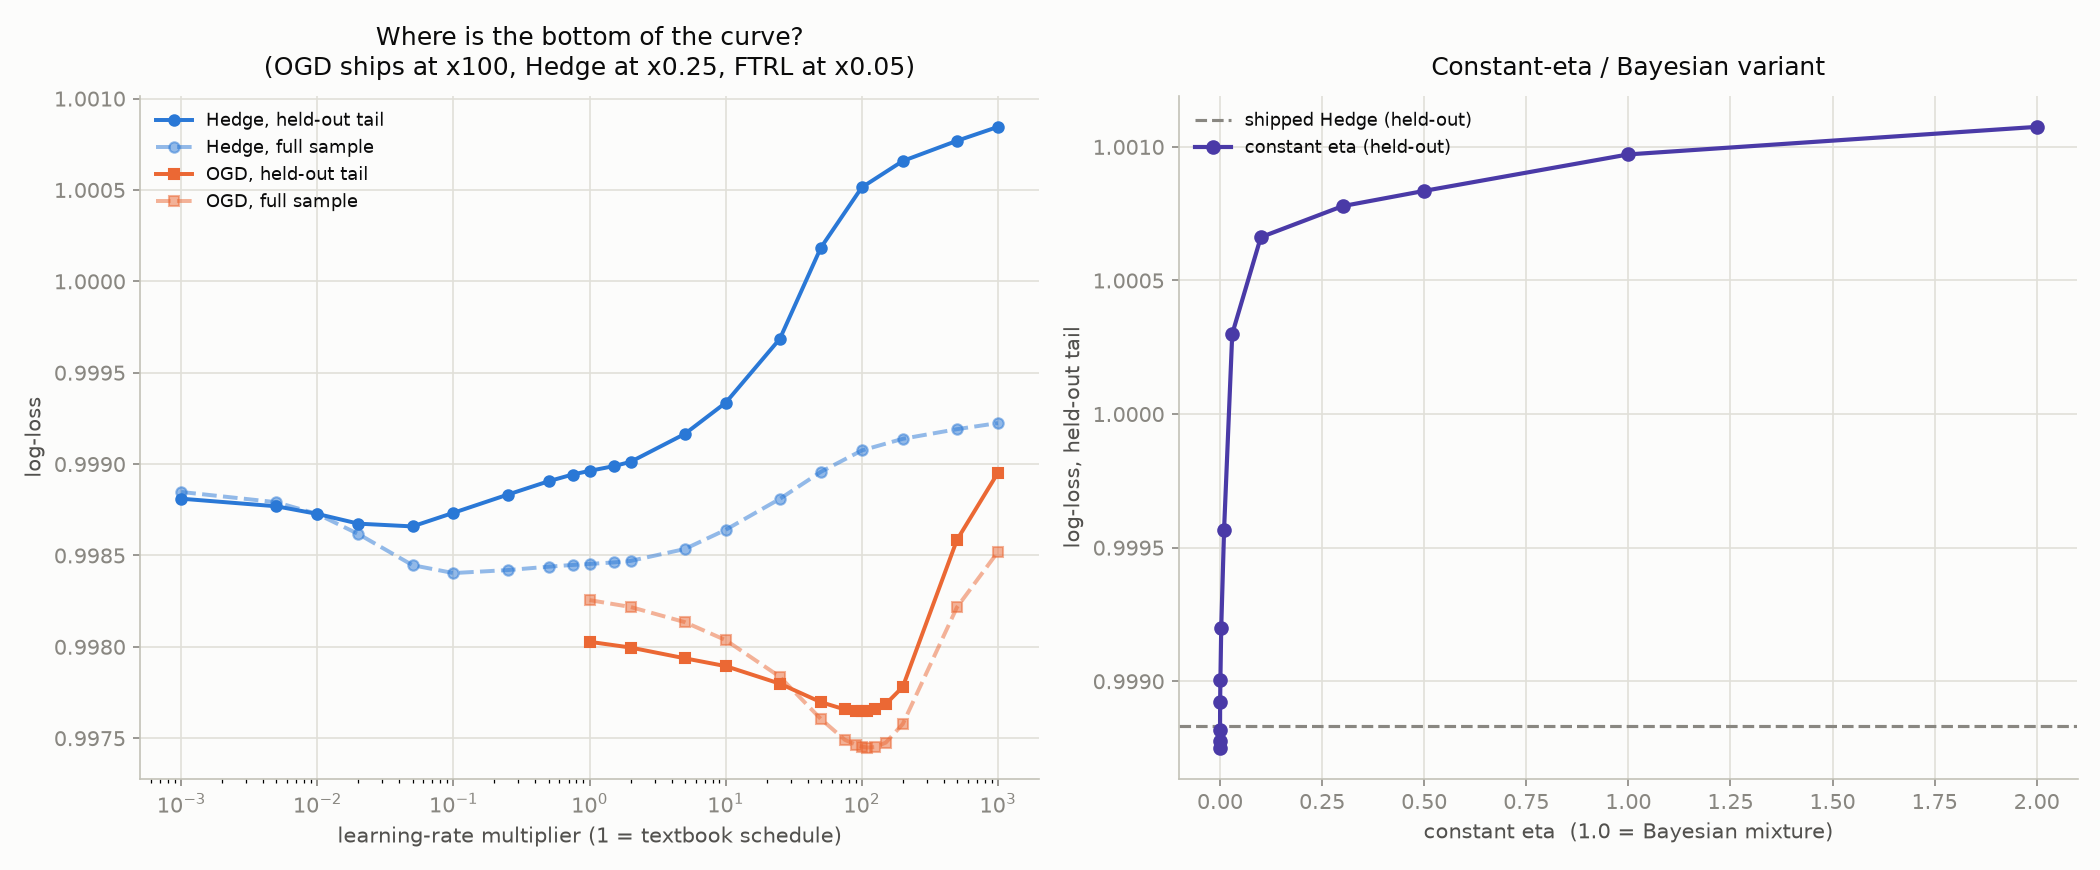
\includegraphics[width=0.92\linewidth]{learning_rate_study.png}
  \caption{Sweep of the step multiplier for all three algorithms. Selection is made on the chronological prefix; the tail is reported as verification. OGD exhibits a genuine interior optimum. The tail curves for Hedge and FTRL keep falling towards the left, but the selection is not made on them; see the remark on the caveat that turned out to be unfounded.}
  \label{fig:lr}
\end{figure}

As Figure~\ref{fig:lr} shows, OGD wants a step a hundred times larger than the theoretical one,
with a genuine interior optimum: a plateau over the range $\times 75$ to $\times 110$, with
$\times 200$, $\times 500$
and $\times 1000$ clearly worse. Hedge and FTRL want a \emph{smaller} step, by factors of 4 and
20 respectively.

\paragraph{A caveat that turned out to be unfounded.} The \emph{tail} minimum for Hedge and FTRL
lies below the values used, at $\times 0.05$ and $\times 0.005$ respectively, and for a time this
thesis carried the caveat that those two algorithms were reported with a sub-optimal step. The
caveat was wrong, and the reason is worth stating: \textbf{selecting on the tail is selecting on
the test set}, which is exactly what the protocol of \S\ref{sec:protocol} exists to prevent.
Because the log-loss is a plain mean over rounds, the prefix figure is recoverable exactly from
the full sample and the tail, as
$(\text{full}\cdot T - \text{tail}\cdot n_{\text{tail}})/n_{\text{train}}$, and under the protocol
the answer reverses: Hedge selects $\times 0.25$ and FTRL $\times 0.05$, that is \emph{exactly}
the multipliers in force.

The numbers also show why. For Hedge, $\times 0.05$ gives a train figure of $0.99838$ against
$0.99828$ for $\times 0.25$; for FTRL, $\times 0.005$ gives $0.99862$ against $0.99828$ for
$\times 0.05$. In both cases the ordering \emph{reverses} between prefix and tail, which is the
signature of fitting the tail rather than evidence of better tuning. OGD remains optimal at
$\times 100$, with $\times 110$ giving an identical tail: a tie inside the plateau already
described.

\paragraph{A constant step: the one schedule idea that had not been tested properly.} The decaying
$1/\sqrt{t}$ is derived for a \emph{static} comparator, whereas the panel here is not static, so a
step that never stops moving is the theoretically indicated alternative. It had been tried only
for Hedge and only over $[0.1, 2]$, while Hedge's decaying schedule passes $\eta \approx 0.033$
at the first round and $\eta \approx 1.7\cdot10^{-4}$ by the middle of the period, i.e. the
entire interesting region lay \emph{below} the old grid. The sweep was extended over five
decades and to all three algorithms, with selection on the prefix and a paired test on the
tail.

\begin{table}[H]
\centering
\begin{tabular}{@{}lrrrrl@{}}
\toprule
& \textbf{constant $\eta$} & \textbf{tail} & \textbf{decaying} & \textbf{$p$} & \\
\midrule
Hedge & $3\cdot10^{-4}$ & 0.99892 & 0.99883 & $<0.001$ & decaying \\
OGD   & $0.1$           & 0.99795 & 0.99765 & $0.021$  & decaying \\
FTRL  & $10^{-5}$       & 0.99879 & 0.99889 & $0.001$  & \textbf{constant} \\
\bottomrule
\end{tabular}
\caption{Constant against decaying step. $\eta$ is selected on the chronological prefix and the
comparison is made on the tail with a moving block bootstrap.}
\label{tab:const-step}
\end{table}

The result is negative for two of them and \textbf{positive for one}. For Hedge and OGD the
constant step loses significantly, by $+0.000089$ and $+0.000299$ respectively. For FTRL, however,
it wins significantly, by $-0.000096$ ($p=0.001$), and the critical point is that the two
schemes have an \emph{identical} score on the prefix ($0.99828$ for both). With nothing to
separate the two on the training data, the selection cannot have favoured the constant step in
order to flatter the tail, and the advantage emerges only out of sample. The explanation is the same asymmetry that explains the opposite tuning directions:
FTRL's $\eta$ multiplies the entire accumulated loss, not one round's gradient, so it is the
one of the three for which ``non-decaying'' means something qualitatively different.

The sweep needed extending here too, for the same reason as before: FTRL's minimum initially sat
on the grid's lower endpoint. Extended down to $10^{-9}$ it became genuinely interior, and the
extension simultaneously confirmed the theoretical limit: as $\eta \to 0$ FTRL degenerates to the
uniform average, and indeed at $\eta=10^{-9}$ it gives $0.99882$, the uniform average's value on
the tail.

\paragraph{A methodological error worth reporting.} The original sweep had the grid
$1, 2, 5, \dots, 1000$ and concluded that Hedge and FTRL were ``already optimal at $\times 1$''.
But $1$ was the \emph{lower endpoint of the grid}, not an optimum, and nobody had looked to the
left of it. Extending downwards revealed genuine interior minima, with gains of $+0.00013$ and
$+0.00018$ respectively on the tail. The conclusion generalises: when a sweep's answer sits at the
endpoint of the grid, the grid must be extended before the answer is believed.

The opposite direction has a structural explanation. OGD's $\eta$ multiplies the gradient of
\emph{one} round, so increasing it means moving further. Hedge's $\eta$ sits in an exponent over
one round's loss, so decreasing it \emph{lengthens the memory}. FTRL's $\eta$ multiplies the
entire accumulated loss, so increasing it collapses it towards follow-the-leader.

\section{Ranking and the choice of panel}

\subsection{Ranking on the full panel}

\begin{table}[H]
\centering
\small
\begin{tabular}{@{}lllrr@{}}
\toprule
& & \textbf{phase} & \textbf{log-loss} & \textbf{Brier} \\
& & & (raw / cal.) & (raw / cal.) \\
\midrule
PSC (Pinnacle) & bookmaker & closing & 0.99714 / 0.99685 & 0.59592 / 0.59577 \\
OGD            & algorithm & ---     & 0.99745 / 0.99693 & 0.59612 / 0.59586 \\
Hedge          & algorithm & ---     & 0.99842 / 0.99773 & 0.59674 / 0.59637 \\
FTRL           & algorithm & ---     & 0.99843 / 0.99774 & 0.59674 / 0.59638 \\
Uniform        & baseline  & ---     & 0.99886 / 0.99813 & 0.59703 / 0.59665 \\
VC\_BV         & bookmaker & opening & 1.00075 / 1.00026 & 0.59833 / 0.59806 \\
WH             & bookmaker & opening & 1.00119 / 1.00048 & 0.59860 / 0.59818 \\
PS (Pinnacle)  & bookmaker & opening & 1.00083 / 1.00055 & 0.59838 / 0.59824 \\
IW             & bookmaker & opening & 1.00186 / 1.00061 & 0.59899 / 0.59826 \\
BW             & bookmaker & opening & 1.00140 / 1.00065 & 0.59873 / 0.59833 \\
B365           & bookmaker & opening & 1.00113 / 1.00073 & 0.59852 / 0.59832 \\
\bottomrule
\end{tabular}
\caption{Ranking by calibrated log-loss, bookmakers with coverage $\geq$70\%.}
\label{tab:ranking}
\end{table}

\begin{figure}[htbp]
  \centering
  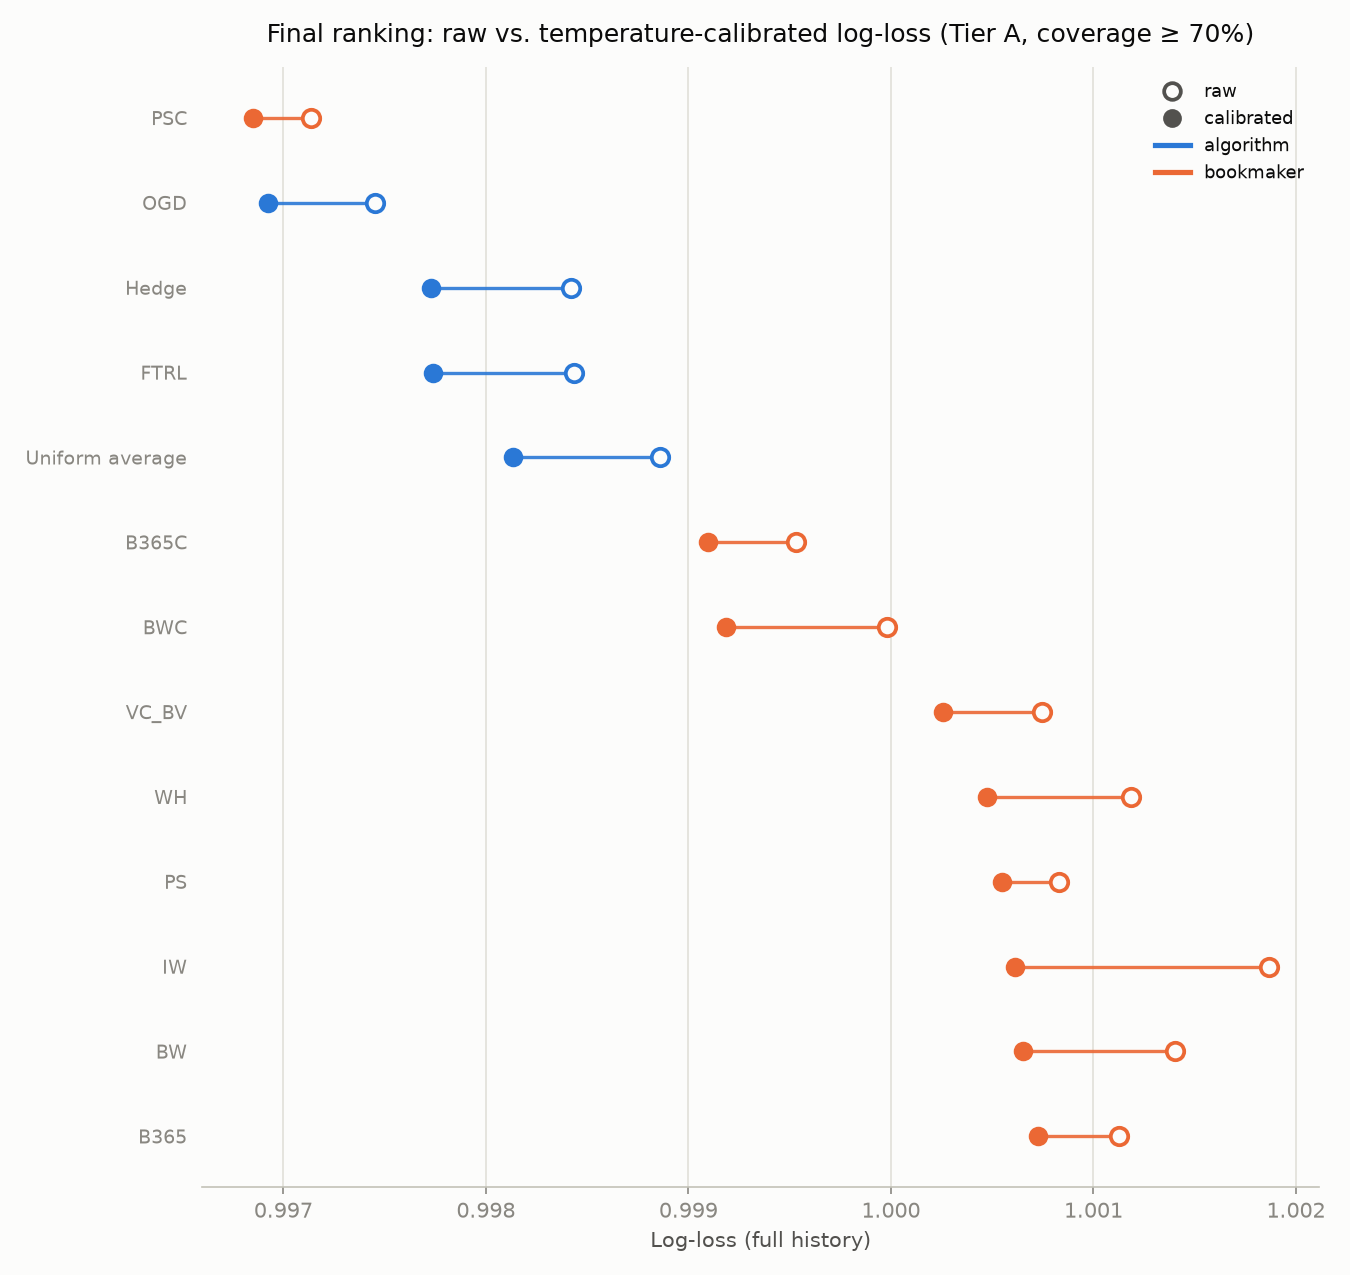
\includegraphics[width=0.92\linewidth]{final_ranking.png}
  \caption{Each row: hollow circle the raw log-loss, filled the calibrated one. The choice of a dot/slope plot rather than a bar chart is deliberate, since log-loss values cluster around $1.0$ with no meaningful zero and a bar chart with a truncated axis would visually exaggerate minute differences.}
  \label{fig:ranking}
\end{figure}

Figure~\ref{fig:ranking} plots the same ranking. The paired tests give:

\begin{itemize}
  \item All three algorithms significantly beat the uniform average: OGD $-0.00141$, Hedge
        $-0.00044$, FTRL $-0.00043$, all $p<0.001$. OGD's margin is about threefold.
  \item OGD significantly beats Hedge ($-0.00097$), FTRL ($-0.00098$) and B365C ($-0.00063$).
  \item Calibration significantly improves all four methods, by $+0.00053$ to $+0.00073$.
  \item PSC remains significantly ahead of OGD in this configuration: $+0.00043$ calibrated,
        $p<0.001$, over the 71,818 common matches.
\end{itemize}

\paragraph{A necessary caveat.} The 70\% coverage threshold leaves in only one closing bookmaker,
PSC, because the remaining closing columns start around 2019/20 and B365C narrowly misses at
69.6\%. The statement ``we beat everyone except PSC'' therefore means, \emph{here}, that we beat
six opening prices. The substantive comparison against closing prices is made in
\S\ref{sec:res-recent} and \S\ref{sec:res-deploy}.

Note that Interwetten occupies the \emph{last} place in the raw log-loss ranking ($1.00186$)
despite having the seventh best coverage. Its addition therefore makes the statement ``we beat
everyone except PSC'' somewhat cheaper, and for that reason the substantive comparison remains
the one against PSC and B365C.

Note also that log-loss and Brier give almost identical orderings, the only exception being the
last two places. Accuracy gives a different ordering, but none of its differences is statistically
significant, as expected, since it is not a proper scoring rule.

\subsection{Which panel}
\label{sec:res-panels}

\begin{table}[H]
\centering
\small
\begin{tabular}{@{}lrrrrrr@{}}
\toprule
& \multicolumn{2}{c}{\textbf{opening} (13)} & \multicolumn{2}{c}{\textbf{all} (26)} & \multicolumn{2}{c}{\textbf{closing} (13)} \\
\cmidrule(lr){2-3}\cmidrule(lr){4-5}\cmidrule(lr){6-7}
& basic & Shin & basic & Shin & basic & Shin \\
\midrule
OGD     & 1.00076 & 1.00024 & 0.99745 & 0.99709 & 0.99722 & 0.99689 \\
Hedge   & 1.00088 & 1.00033 & 0.99842 & 0.99781 & 0.99762 & 0.99714 \\
FTRL    & 1.00088 & 1.00033 & 0.99843 & 0.99782 & 0.99761 & 0.99714 \\
Uniform & 1.00080 & 1.00022 & 0.99886 & 0.99824 & 0.99748 & 0.99703 \\
\bottomrule
\end{tabular}
\caption{Log-loss by panel and de-vig method.}
\end{table}

\begin{figure}[htbp]
  \centering
  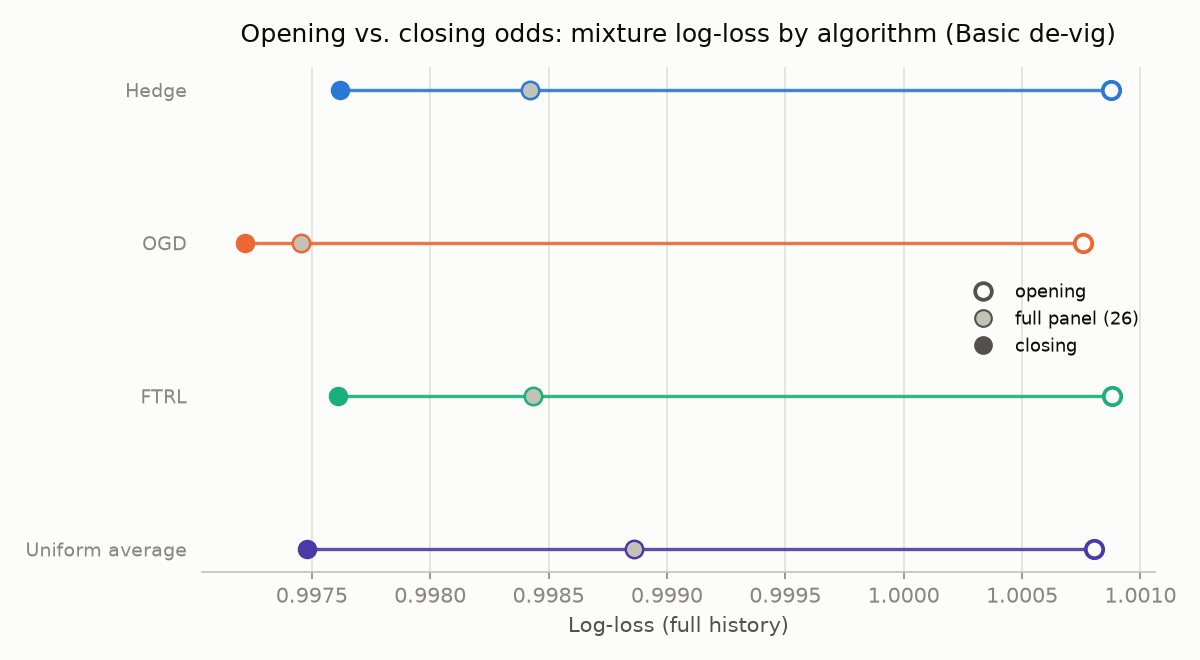
\includegraphics[width=0.92\linewidth]{opening_vs_closing.png}
  \caption{Comparison of the three panels for each algorithm. The ordering closing $<$ all $<$ opening holds in every case.}
  \label{fig:panels}
\end{figure}

As Figure~\ref{fig:panels} makes visible, the ordering closing $<$ all $<$ opening holds
in every cell, and in all 24 comparisons (4
algorithms $\times$ 3 comparisons $\times$ 2 normalisations) the difference is statistically
significant. That closing prices beat opening ones is expected. What is unexpected is that the
closing-only panel also beats the \emph{full} one: the opening bookmakers do not act as useful
diversification but as pure dead weight in the mixture.

Comparing each algorithm with the plain average \emph{inside} the same panel explains the
mechanism and is, in our view, the most generally useful finding of the thesis:

\begin{itemize}
  \item On the \textbf{full} panel all three algorithms significantly beat the average.
  \item On the \textbf{restricted} panels Hedge and FTRL \emph{significantly lose} to the
        average, in 8 tests out of 8. OGD wins on closing and ties on opening.
\end{itemize}

The full panel contains 13 good closing and 13 systematically worse opening experts, that is a
clear quality difference available to be learned. In a homogeneous panel that difference is
absent, and for two of the three algorithms the adaptation costs more than it returns.

\subsection{Where exactly closing prices are superior}
\label{sec:res-arrival}

\S\ref{sec:res-panels} shows that the closing panel wins by $\sim0.0035$ in log-loss. That is an
average, and Remark~\ref{rem:closing} makes a sharper prediction: if the superiority is due to
information arrival, it must be concentrated where the price \emph{actually moved}. To test this,
each match is characterised by the total variation distance between the initial and the final
probability distribution of each house, averaged over the 13 available opening/closing pairs, and
the matches are split into quintiles.

\begin{table}[H]
\centering
\small
\begin{tabular}{@{}lrrrrr@{}}
\toprule
\textbf{Movement quintile} & Q1 & Q2 & Q3 & Q4 & Q5 \\
\midrule
Mean movement & 0.0082 & 0.0144 & 0.0215 & 0.0324 & 0.0598 \\
log-loss opening & 0.99161 & 1.00581 & 1.00068 & 1.00666 & 1.00790 \\
log-loss closing & 0.99118 & 1.00509 & 0.99868 & 1.00214 & 0.99632 \\
\midrule
\textbf{closing $-$ opening} & $-0.00044$ & $-0.00072$ & $-0.00200$ & $-0.00452$ &
$\mathbf{-0.01158}$ \\
$p$ & 0.052 & 0.050 & $<0.001$ & $<0.001$ & $<0.001$ \\
\bottomrule
\end{tabular}
\caption{Closing advantage by quintile of line movement, 10,649--10,650 matches per quintile.}
\label{tab:arrival}
\end{table}

\begin{figure}[H]
\centering
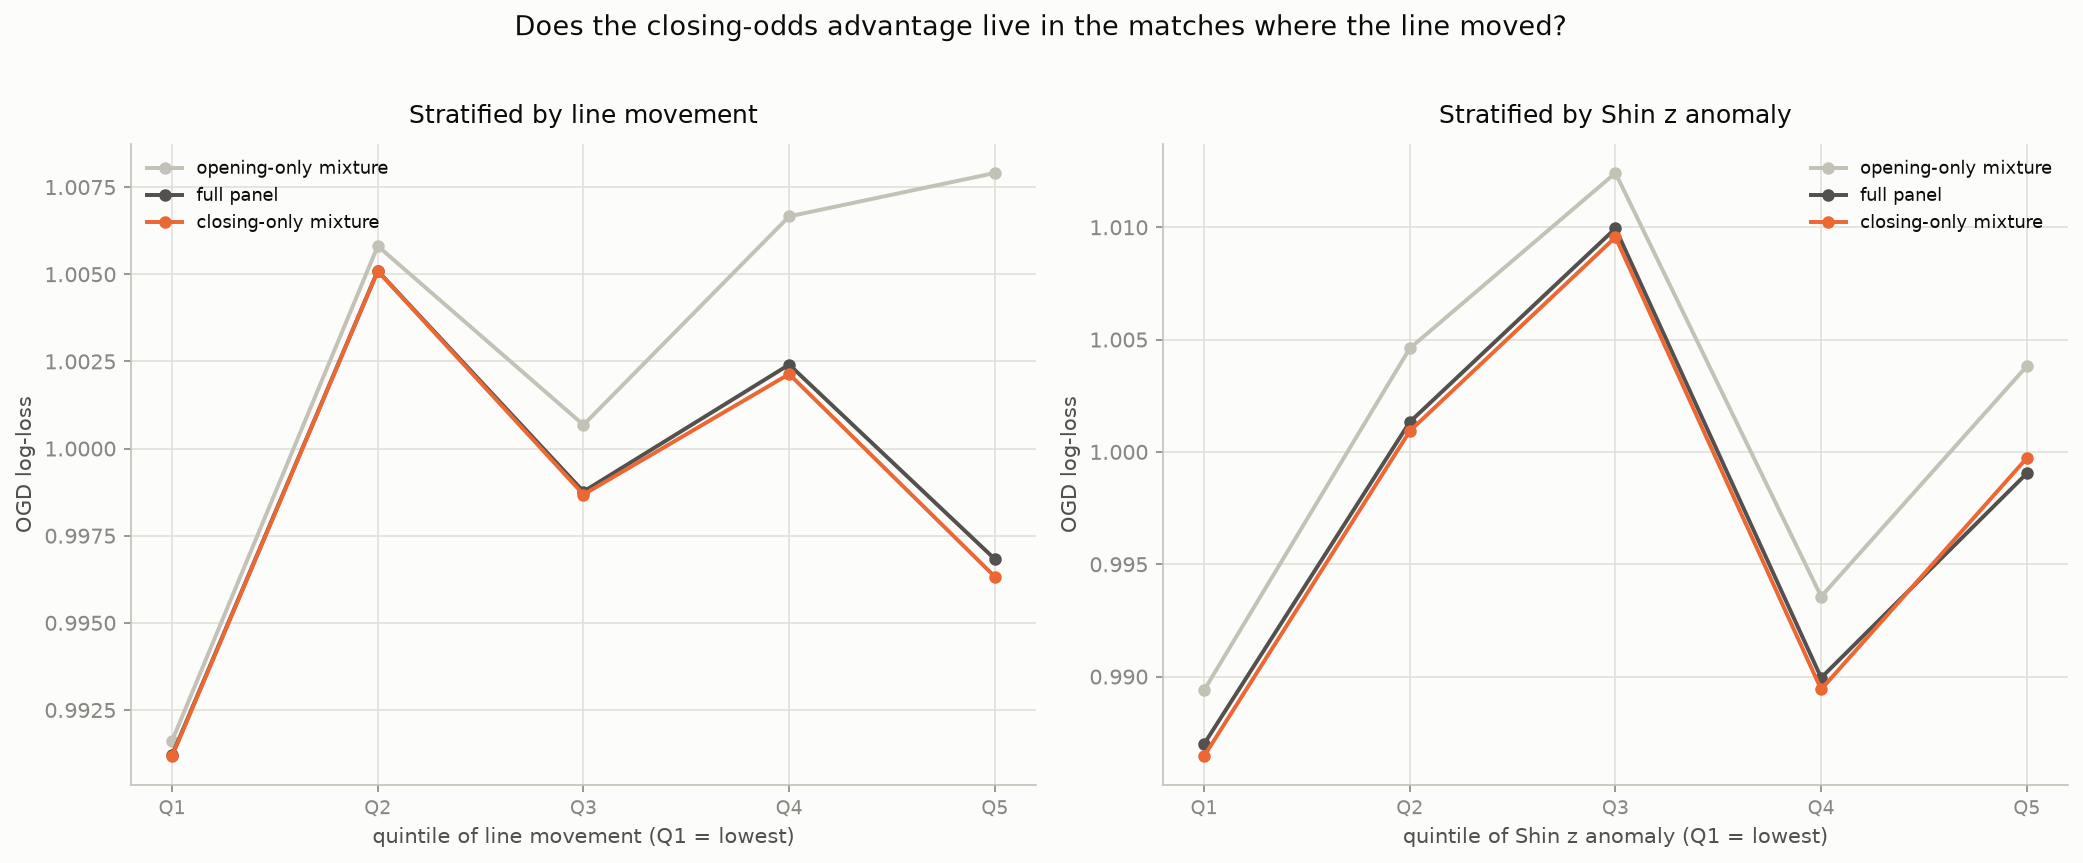
\includegraphics[width=\textwidth]{information_arrival.png}
\caption{Left, the stratification by line movement; right, by anomaly of Shin's $z$.}
\end{figure}

\paragraph{The prediction is confirmed, with a 26-fold gradient.} The closing advantage runs from
$-0.00044$ in the quiet fifth of the matches to $-0.01158$ in the noisy one. In Q1 it is in fact
\textbf{not even statistically significant} ($p=0.052$): in the fifth of matches where the line
barely moved, there is no measurable closing advantage. The ``superiority of closing prices'' is
therefore not a general property of final prices but a phenomenon of the top quintile.

\paragraph{A necessary caveat.} Movement is measured from the \emph{same} closing prices that the
closing panel uses, so the null result in Q1 is partly mechanical: if the two prices nearly
coincide, the two mixtures cannot differ much. The non-trivial part is the \emph{direction} at
the other extreme. A large movement could perfectly well go the wrong way; that the later price
is systematically the better one by $0.0116$ is exactly the market-efficiency claim, localised
where it actually operates. A useful control: the \emph{difficulty} of the matches is not
monotone across the quintiles (the full panel's log-loss runs $0.99120$, $1.00510$, $0.99877$,
$1.00241$, $0.99683$), whereas the advantage is, so the gradient is not an artefact of the form
``harder matches, larger differences''.

\paragraph{Shin's $z$ is a much weaker indicator.} Stratifying instead by the anomaly of $z$
(the quantity that \S\ref{sec:microstructure-theory} identifies with the estimated proportion
of informed traders) the gradient is only $-0.00295$ to $-0.00498$, that is a factor of $1.7$
against $26$, with all quintiles significant. So $z$ does detect something, but the actual
price movement is an incomparably cleaner indicator that information has arrived, reasonably
so, since $z$ is estimated from a single moment of the market whereas movement observes the
difference of two.

\subsection{The configuration that is selected}
\label{sec:res-config}

Three improvements had been measured separately (the corrected step, the closing-only panel,
Shin) and are combined here. Every configuration is scored on the same 71,818 matches, the
intersection of all of them with PSC, following the principle of \S\ref{sec:common-rounds}.

\begin{table}[H]
\centering
\begin{tabular}{@{}lrrr@{}}
\toprule
\textbf{Configuration} & \textbf{full} & \textbf{train} & \textbf{25\% tail} \\
\midrule
PSC alone                            & 0.99685 & 0.99746 & 0.99502 \\
closing-only $+$ Shin                & 0.99692 & 0.99754 & 0.99507 \\
closing-only, proportional           & 0.99693 & 0.99756 & 0.99506 \\
closing-only $+$ Shin, no single-season & 0.99692 & 0.99754 & 0.99509 \\
full panel, proportional             & 0.99728 & 0.99801 & 0.99508 \\
full panel, Shin                     & 0.99731 & 0.99804 & 0.99512 \\
\bottomrule
\end{tabular}
\caption{Calibrated log-loss of OGD by configuration, the same 71,818 matches throughout.}
\end{table}

\begin{figure}[htbp]
  \centering
  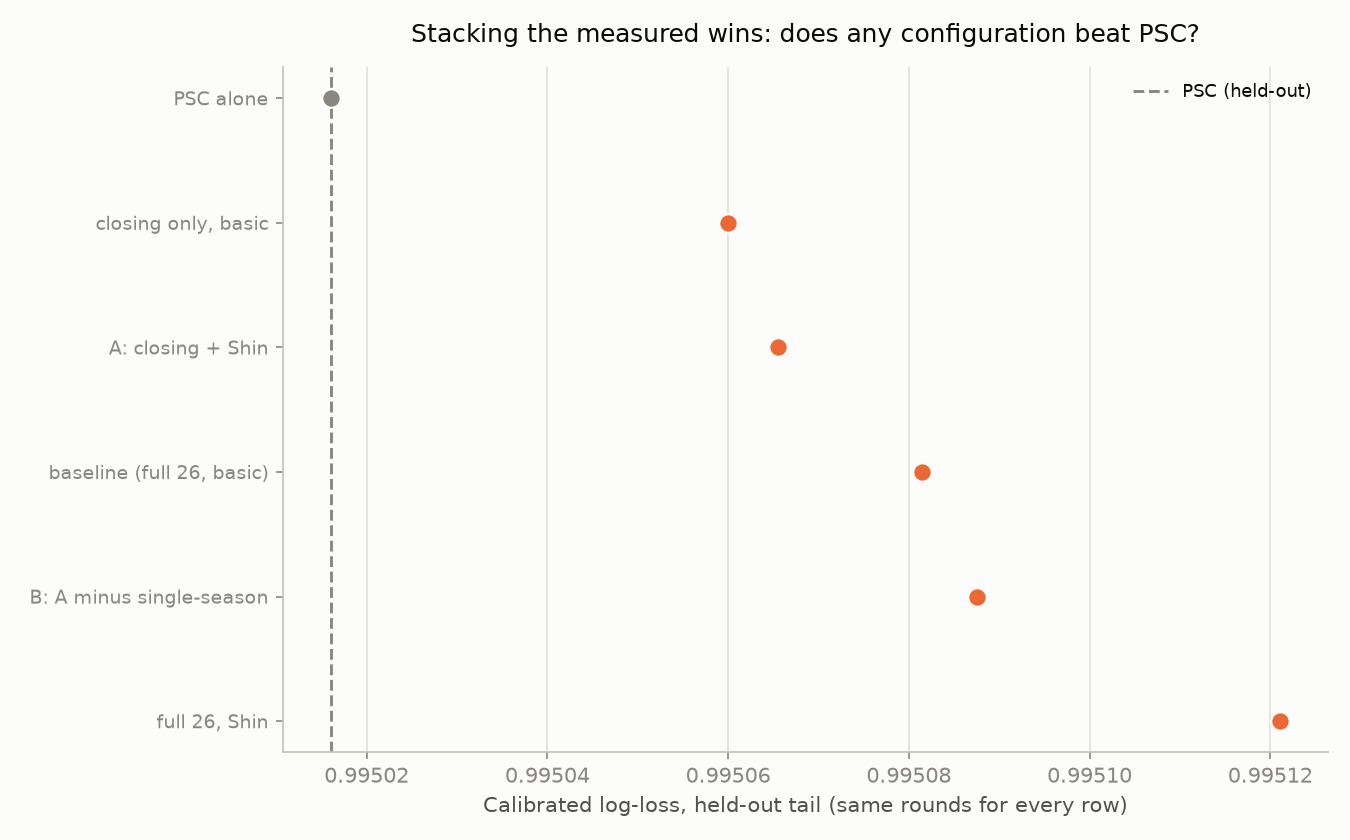
\includegraphics[width=0.92\linewidth]{best_configuration.png}
  \caption{The configurations on the held-out tail, with PSC as the reference line. All of them cluster within $0.00005$.}
  \label{fig:bestconfig}
\end{figure}

\begin{itemize}
  \item \textbf{The panel does all the work.} Closing-only $+$ Shin beats the full panel by
        $-0.00036$ ($p<0.001$), and closing-only with proportional normalisation by $-0.00034$
        ($p<0.001$).
  \item \textbf{Shin on its own offers nothing measurable} over the full panel ($+0.00004$,
        $p=0.181$), consistent with Shin and temperature scaling correcting the same
        favourite-longshot bias, so that the second absorbs the first.
  \item \textbf{Against PSC}: the full panel significantly loses ($+0.00043$, $p<0.001$), while
        closing-only $+$ Shin \emph{ties} ($+0.00007$, $p=0.234$) and closing-only with
        proportional normalisation likewise ($+0.00009$, $p=0.143$).
\end{itemize}

The 25\% tail does not produce a winner: all six rows gather within less than $0.00005$
(Figure~\ref{fig:bestconfig}). It thus
confirms the tie, and it would not be honest to present it as a win. Note also that in every
closing configuration PSC is \emph{inside} the mixture: ``we reach PSC'' reads as ``the mixture
reaches its own best member''.

\subsection{Without Pinnacle}
\label{sec:res-nopinnacle}

The obvious counter-argument is that the mixture merely reproduces Pinnacle, which is inside it
anyway. Removing both of its columns and refitting from scratch on three panels:

\begin{table}[H]
\centering
\small
\begin{tabular}{@{}llrll@{}}
\toprule
\textbf{Panel} & \textbf{OGD rank} & \textbf{log-loss} & \textbf{First} & \textbf{Paired} \\
\midrule
full (24)         & \#3 of 9 & 0.99782 & FTRL 0.99771   & 5 wins, 0 losses \\
closing-only (12) & \#1 of 9 & 0.99919 & OGD (itself)   & 3 wins, 2 ties \\
opening-only (12) & \#5 of 9 & 0.99999 & VC\_BV 0.99987 & 3 wins, \textbf{1 loss}, 1 tie \\
\bottomrule
\end{tabular}
\caption{Each panel is refitted from scratch and compared against the bookmakers of its own
phase.}
\end{table}

\begin{figure}[htbp]
  \centering
  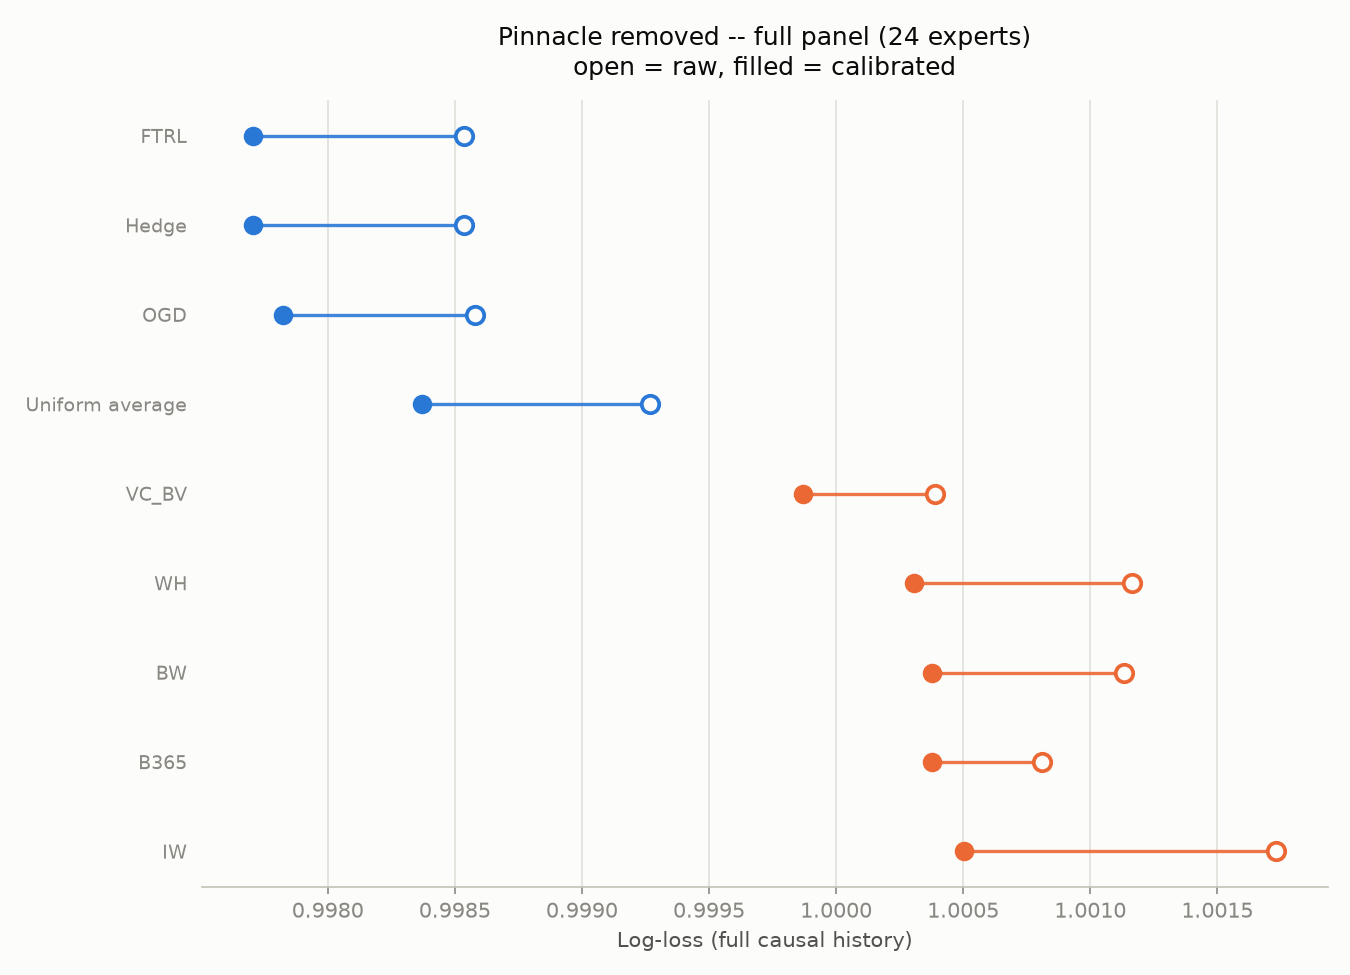
\includegraphics[width=0.92\linewidth]{no_pinnacle.png}
  \caption{Full panel without any Pinnacle column. All four methods sit above all remaining bookmakers.}
  \label{fig:nopinn}
\end{figure}

On the \textbf{full} panel the result holds comfortably (Figure~\ref{fig:nopinn}): all four
methods sit above every
bookmaker, and OGD significantly beats all \emph{five}, with margins from $-0.00181$ (VC\_BV) to
$-0.00315$ (IW) and $p<0.001$ throughout. All of them, however, are opening prices.

On the two \textbf{homogeneous} panels the result changes. On closing, OGD beats three (WHC
$-0.00088$, IWC $-0.00077$, BWC $-0.00051$) and ties with B365C ($p=0.505$) and VC\_BVC
($p=0.284$); it does rank first, but with the plain average second at a distance of $0.00002$,
i.e. practically indistinguishable. On opening it again beats three, ties with B365 ($p=0.203$),
but \textbf{significantly loses to VC\_BV} ($+0.00030$, $p=0.004$): the only case in the whole
thesis where a \emph{bookmaker} other than Pinnacle significantly beats us, and there the plain
average moves ahead of OGD. The statement is deliberately restricted to bookmakers: in the
deployment test (\S\ref{sec:res-deploy}) Betfair Exchange also significantly beats us, but that
is not a bookmaker but an exchange.

The pattern is stable enough not to be attributed to chance, and it repeats the finding of
\S\ref{sec:res-panels}: once Pinnacle leaves, the remaining members of the same phase resemble one
another so closely that no quality difference is left to learn. The configuration that is
selected is therefore the best partly \emph{because} it contains the market's best odds-setter.

\section{Robustness over time}

\subsection{Recent window}
\label{sec:res-recent}

The coverage threshold is defined over the decade, which favours whoever was quoting long ago.
Restricting to the last five seasons (38,749 matches), B365C, BWC, VC\_BVC and WHC all pass the
threshold and the demanding comparison becomes possible.

\begin{table}[H]
\centering
\small
\begin{tabular}{@{}rllr@{}}
\toprule
\textbf{\#} & \textbf{Series} & \textbf{phase} & \textbf{log-loss} \\
\midrule
1 & PSC & closing & 0.99439 \\
2 & \textbf{OGD} & --- & \textbf{0.99495} \\
3 & VC\_BVC & closing & 0.99498 \\
4 & WHC & closing & 0.99502 \\
5 & BWC & closing & 0.99504 \\
6 & B365C & closing & 0.99543 \\
7 & Uniform & --- & 0.99591 \\
8 & Hedge & --- & 0.99604 \\
9 & FTRL & --- & 0.99607 \\
10--14 & WH, PS, VC\_BV, BW, B365 & opening & 0.99771 and below \\
\bottomrule
\end{tabular}
\caption{Last five seasons, full panel, calibrated log-loss.}
\end{table}

\begin{figure}[htbp]
  \centering
  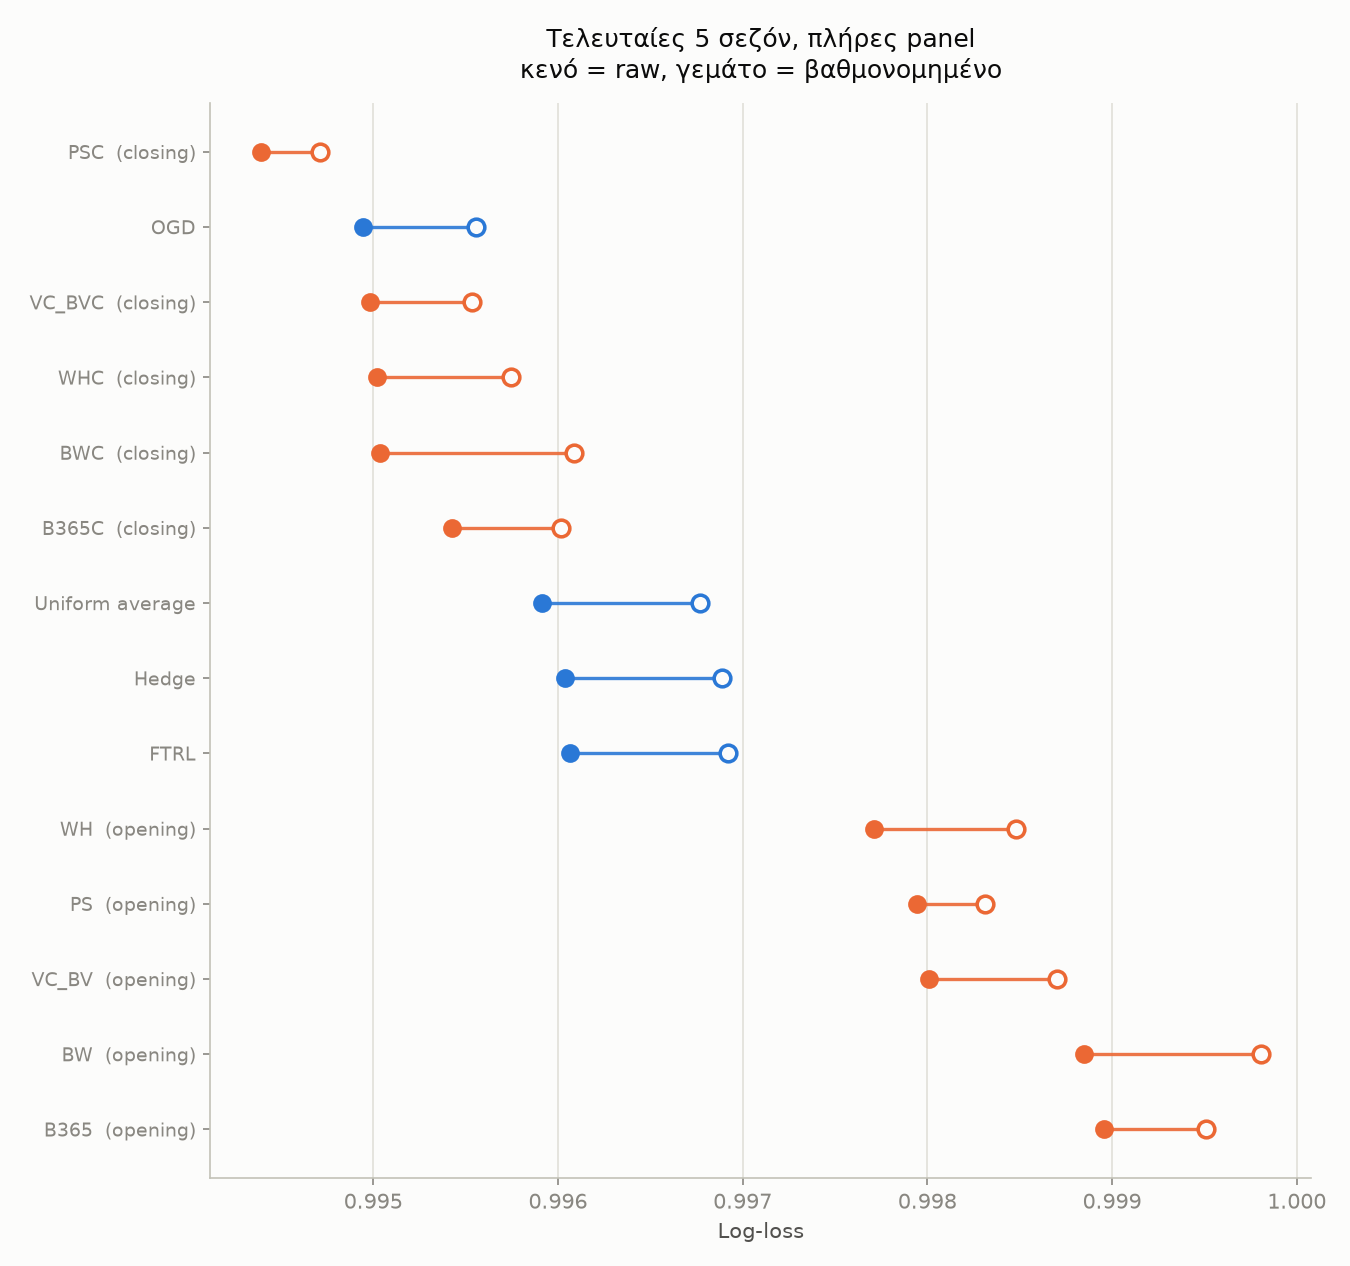
\includegraphics[width=0.92\linewidth]{recent_window.png}
  \caption{Last five seasons. The closing bookmakers now pass the coverage threshold and the comparison becomes more demanding.}
  \label{fig:recent}
\end{figure}

OGD sits at \#2 (Figure~\ref{fig:recent}), ahead of every closing bookmaker other than
Pinnacle, and the gap to PSC shrinks
to $+0.00036$ ($p=0.014$) from the decade's $+0.00043$. Two findings, however, \emph{reverse} and
are reported explicitly: Hedge and FTRL lose to the plain average on \emph{all} panels here, not
only the restricted ones ($+0.00012$ and $+0.00015$, $p=0.006$ and $p=0.002$), and log-loss and
Brier cease to agree on the ordering.

\subsection{Deployment test}
\label{sec:res-deploy}

The test with a real date cut: fitting on 65,009 rounds up to 31/12/2024, measurement on 11,574
rounds of 2025--26, of which 8,151 are common. Figure~\ref{fig:deploy} plots the outcome.

\begin{table}[H]
\centering
\small
\begin{tabular}{@{}rllr@{}}
\toprule
\textbf{\#} & \textbf{Series} & \textbf{phase} & \textbf{log-loss} \\
\midrule
1 & BFEC (Betfair Exchange) & closing & 1.00040 \\
2 & \textbf{OGD closing-only, online} & --- & \textbf{1.00110} \\
3 & OGD full panel, online & --- & 1.00129 \\
4 & BWC & closing & 1.00146 \\
5 & OGD closing-only, frozen & --- & 1.00151 \\
6 & B365C & closing & 1.00165 \\
7 & OGD full panel, frozen & --- & 1.00183 \\
8--10 & B365, BW, BFE & opening & 1.00371 -- 1.00758 \\
\bottomrule
\end{tabular}
\caption{Trained up to 31/12/2024, measured on 2025--26.}
\end{table}

\begin{figure}[htbp]
  \centering
  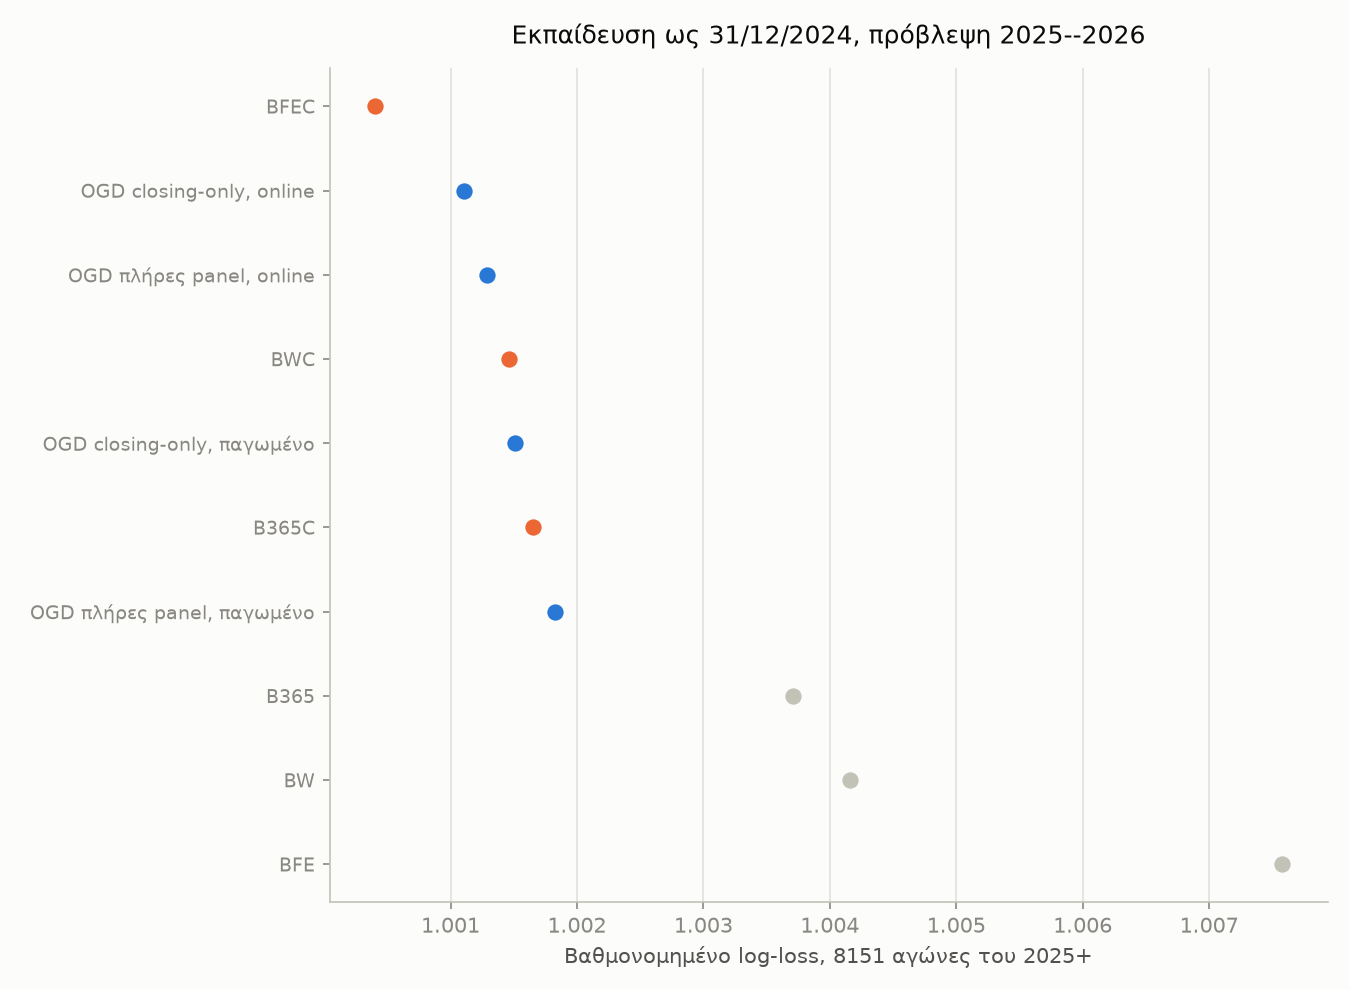
\includegraphics[width=0.92\linewidth]{deployment_test.png}
  \caption{Deployment test. The opening prices sit clearly lower, while the closing prices and the variants of the mixture cluster together.}
  \label{fig:deploy}
\end{figure}

\begin{itemize}
  \item \textbf{Every opening price is significantly beaten}, in every variant: $-0.0019$ to
        $-0.0065$, all $p\leq0.019$.
  \item \textbf{The closing prices are not beaten.} The best outcome is a tie with all three, and
        only in the closing-only / online variant: B365C $p=0.193$, BWC $p=0.361$, BFEC
        $p=0.052$. In the full-panel variants \textbf{BFEC significantly beats us} ($+0.00089$,
        $p=0.013$ online; $+0.00143$, $p=0.002$ frozen), so the tie with every closing price
        holds only for the closing-only variant.
  \item The online variant consistently beats the frozen one ($1.00110$ against $1.00151$), so
        the precise statement is not ``trained up to 2024'' but ``runs continuously''.
\end{itemize}

\paragraph{Pinnacle in this window.} Its coverage drops to 59\% after 2025 and it stops quoting on
14/01/2026, so it does not pass the threshold. Forcing it into the common table drops the common
matches from 8,151 to 2,860 and no result remains significant. It is therefore compared one to
one, over its own rounds: we significantly beat PS ($-0.0022$ to $-0.0023$, $p$ from $0.007$ to
$0.019$, over 6,857 matches), and we tie with PSC ($p$ from $0.532$ to $0.796$, over 6,892
matches).

It is worth noting that the best forecaster in this window is not a bookmaker but \textbf{Betfair
Exchange}: an exchange where players bet against one another, that is a market price without an
operator's margin.

\section{Value betting and the learned stake size}
\label{sec:res-value}

A Kelly simulation with calibrated probabilities and a panel matched to the target's phase. The
stake size is not pinned to a fixed fraction but learned online, with the multiplier of
\S\ref{sec:oco-kelly-theory}; the fixed coefficient $\tfrac14$ is retained as a reference point.

\paragraph{Correctness check and selection.} A constant $\lambda = 0.25$ reproduces the
implemented simulation \emph{exactly}, at every round of deployment and over the same set of
bets, so the learned multiplier is the only difference between the columns that follow. The rate,
the initial value and the upper bound of $\lambda$ are selected on a chronological $75\%$ prefix
of the \emph{bets}, jointly for all targets, and the remaining tail stays outside the selection.
Neither of the two preceding stages is re-tuned here.

The selection gives $\lambda_0 = 0.5$ and $\lambda_{\max} = 1.5$ for Online Newton Step, with a
tail of $+0.000106$ in log growth rate per bet, and $\lambda_0 = 0.25$, $\lambda_{\max} = 1$ for
OGD, with a tail of $+0.000101$. One point is worth noting that contradicts every other tuning in
the thesis: \textbf{Online Newton Step selects a rate multiplier equal to $1$}, that is the
constant the theory supplies needs no correction at all, whereas OGD needs $\times 10$ and in one
setting the grid runs off the edge without stabilising. Where the structure of the loss is
exploited correctly, the a-priori bound turns out to be correctly calibrated as well.

\begin{table}[H]
\centering
\small
\begin{tabular}{@{}lrrrrr@{}}
\toprule
\textbf{Against} & \textbf{Bets} & \textbf{Kelly $\tfrac14$} & \textbf{OCO $\lambda$} &
\textbf{Full Kelly} & \textbf{mean $\lambda$} \\
\midrule
WHC     &  7,253 & $84.2\times$  & $\mathbf{6{,}494\times}$ & $29{,}342\times$ & 0.79 \\
BWC     &  6,920 & $3.09\times$  & $\mathbf{7.08\times}$    & $13.77\times$    & 0.62 \\
VC\_BVC &  4,561 & $1.58\times$  & $1.54\times$             & $1.74\times$     & 0.57 \\
B365C   &  7,643 & $1.05\times$  & $0.67\times$             & $0.24\times$     & 0.39 \\
PSC     & 19,497 & $0.54\times$  & $0.25\times$             & $0.0035\times$   & 0.37 \\
\bottomrule
\end{tabular}
\caption{Final bankroll starting from $1$, calibrated probabilities, proportional normalisation.
Every column plays the \emph{same} bets, since the choice of outcome does not depend on the size.
The last column is the mean multiplier learned by Online Newton Step.}
\label{tab:oco-kelly}
\end{table}

\begin{figure}[H]
\centering
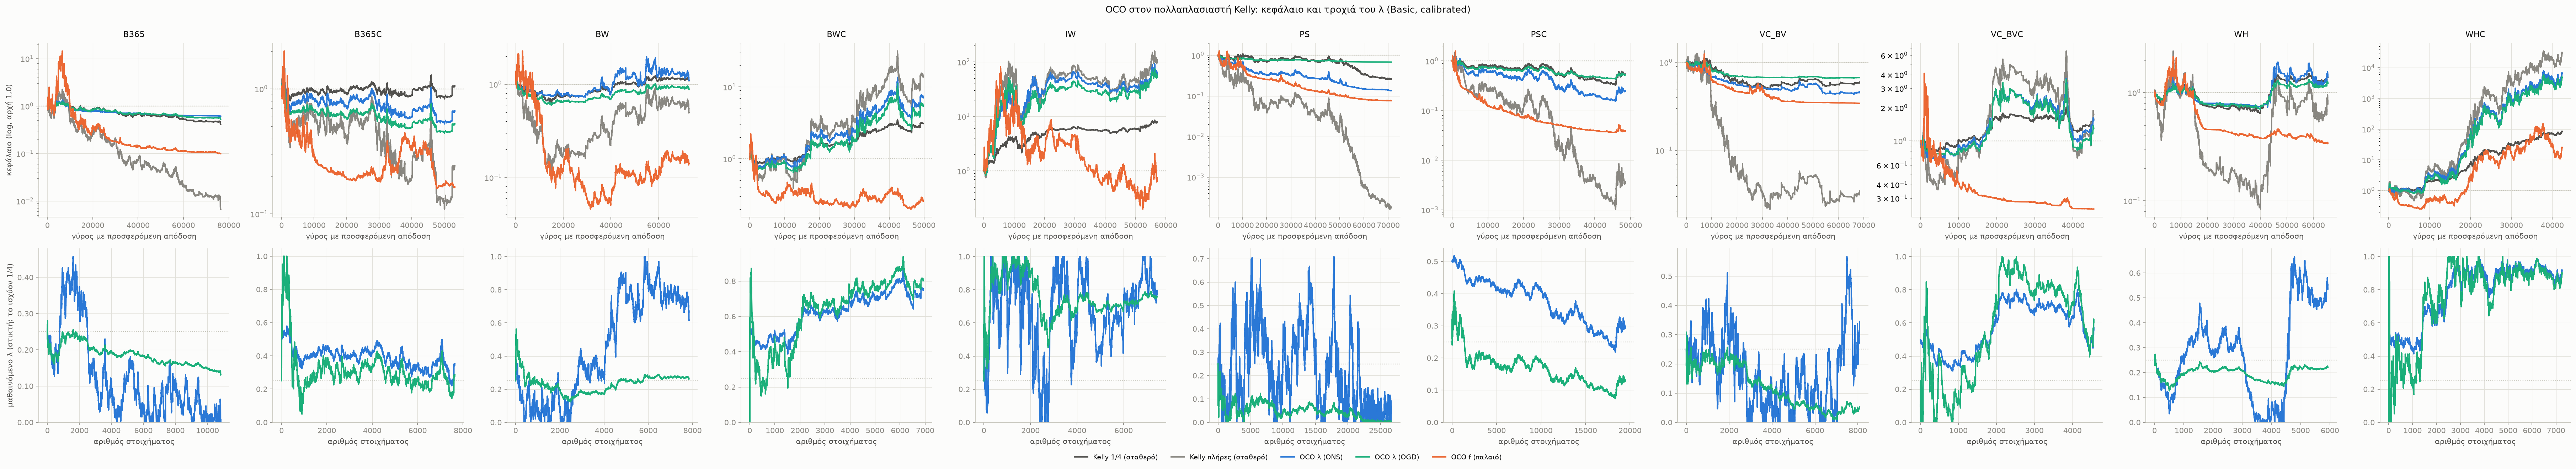
\includegraphics[width=\textwidth]{oco_kelly.png}
\caption{Above, the path of the bankroll; below, the trajectory of the learned $\lambda$ with a
dotted line at the $\tfrac14$ in force.}
\end{figure}

\paragraph{The result has two parts that do not say the same thing.} On the closing targets, in
the per-bet paired test the learned multiplier \textbf{ties} with the fixed $\tfrac14$: over
twenty cells (two normalisations $\times$ two stages $\times$ five targets) there are 17 ties, two
wins and one loss. In final bankroll it is ahead on two of the five targets, and on WHC by seventy-seven
times. The two reconcile numerically: the per-bet difference is $+0.00060$, minute, but it
compounds over $7{,}253$ bets, while the uncertainty remains wide enough that the test does not
certify it ($p=0.099$). It is the same pattern as the ``sharp'' anchor-bookmaker result:
systematic superiority in the point estimate, without statistical certification.

\paragraph{What the multiplier learns.} Against the closing targets it sits almost everywhere
above $\tfrac14$, and its value tracks how profitable the target is: $0.37$ against the
loss-making PSC, $0.79$ against the profitable WHC. It therefore raises the risk where there is an edge and pulls it back where there
is none, behaviour no constant can express, and which emerges without its being given any
information about who the opponent is.

\paragraph{The formulation was the problem, not the idea.} The same question had been posed
earlier with the learner learning the \emph{fraction} of capital directly. That version lost
systematically: 9 losses out of 20 cells, no wins. The cause is exactly the one
\S\ref{sec:oco-kelly-theory} predicts; the comparator ``best constant stake'' does not contain
the closed form, and the learner throws away the $\hat{p}_t$ that the two preceding stages have
just produced. Changing only what is learned, with the same data and the same test, the result
goes from systematic loss to a tie with a point-estimate advantage.

\paragraph{A side finding: $\tfrac14$ is excessively conservative.} \emph{Full} Kelly ties in 16 of
the 20 cells, wins in 2 and loses in only 2. Its risk is concentrated almost entirely on PSC,
where it wipes out the bankroll ($0.0035$). On the profitable targets, that is, the fixed
$\tfrac14$ leaves a substantial part of the growth unused. The learned multiplier is the middle
road: it keeps most of the upside and avoids the catastrophe.

\paragraph{Where there is an edge.} Which bookmakers are beatable at all is mapped over ten
targets with the fixed $\tfrac14$, so that the rows stay comparable with one another.

\begin{table}[H]
\centering
\small
\begin{tabular}{@{}llrrrl@{}}
\toprule
\textbf{Against} & \textbf{Phase} & \textbf{Bets} & \textbf{Bankroll} & \textbf{$p$} & \\
\midrule
WHC     & closing & 6,565  & $38.52\times$ & $<0.001$ & profit \\
IW      & opening & 7,443  & $7.89\times$  & $0.008$  & profit \\
\midrule
BWC     & closing & 6,607  & $1.81\times$  & $0.247$ & --- \\
WH      & opening & 5,931  & $1.38\times$  & $0.545$ & --- \\
BW      & opening & 7,841  & $1.09\times$  & $0.820$ & --- \\
VC\_BVC & closing & 4,653  & $0.75\times$  & $0.455$ & --- \\
VC\_BV  & opening & 8,083  & $0.60\times$  & $0.245$ & --- \\
B365C   & closing & 7,970  & $0.58\times$  & $0.328$ & --- \\
B365    & opening & 10,829 & $0.41\times$  & $0.101$ & --- \\
PS      & opening & 26,675 & $0.26\times$  & $0.055$ & --- \\
\midrule
PSC     & closing & 39,997 & $0.0002\times$ & $<0.001$ & loss \\
\bottomrule
\end{tabular}
\caption{The $p$ column concerns the mean log growth rate per bet. The final bankrolls are not
comparable across rows, since the number of bets differs by an order of magnitude.}
\end{table}

Over eleven bookmakers there are \emph{two} significant profits (both against ``soft'',
recreational-facing houses) and one significant loss, against PSC, which is the best forecaster
in the panel and therefore exactly the opponent an inferior model ought to lose to. The test
thus works in both directions. Phase matching is essential: with the full panel instead of the
closing-only one, the result gets worse on \emph{every} closing target.

\paragraph{The extension to opening targets.} The learned multiplier is applied to all six opening
targets as well, with the corresponding opening-only panel. The causality requirement is stricter
here: removing the target is not enough, the \emph{whole} closing side must go, since no closing
price exists at the moment the bet is placed. The hyperparameters are selected separately per
phase, on that phase's own prefix of bets, so that the opening result does not depend on closing
bets it is supposed to be independent of.

\begin{table}[H]
\centering
\small
\begin{tabular}{@{}lrrrrr@{}}
\toprule
\textbf{Against} & \textbf{Bets} & \textbf{Kelly $\tfrac14$} & \textbf{OCO $\lambda$} &
\textbf{Full Kelly} & \textbf{mean $\lambda$} \\
\midrule
IW      &  7,443 & $7.89\times$  & $\mathbf{64.4\times}$ & $109.6\times$  & 0.67 \\
WH      &  5,931 & $1.38\times$  & $1.39\times$          & $0.78\times$   & 0.28 \\
BW      &  7,841 & $1.09\times$  & $1.10\times$          & $0.50\times$   & 0.45 \\
VC\_BV  &  8,083 & $0.60\times$  & $0.67\times$          & $0.03\times$   & 0.17 \\
B365    & 10,829 & $0.41\times$  & $0.61\times$          & $0.007\times$  & 0.12 \\
PS      & 26,675 & $0.26\times$  & $\mathbf{0.68\times}$ & $0.0003\times$ & 0.05 \\
\bottomrule
\end{tabular}
\caption{Opening targets: final bankroll starting from $1$, calibrated probabilities,
proportional normalisation. The OCO $\lambda$ column gives the better of the two variants
(ONS / OGD) and the mean $\lambda$ corresponds to it.}
\label{tab:oco-kelly-opening}
\end{table}

The finding is that the learned multiplier pays off \emph{more} on opening prices than on closing
ones: 8 wins and 2 losses over 48 paired tests, against 4 wins and 3 losses on the closing side.
Significant wins arise against PS ($p<0.001$), IW ($p=0.027$) and VC\_BV ($p=0.009$), while the
two losses are minute ($-0.000028$ and $-0.000080$).

More interesting than the result is the \emph{mechanism}, which becomes visible here. The mean
$\lambda$ ranks the targets almost perfectly by how beatable they are, without the algorithm being
given any information about who the opponent is: against IW, the only profitable opening target,
it raises $\lambda$ to $0.67$, that is nearly full Kelly; against PS, the hardest, it lowers it to
$0.05$ and essentially stops betting, thereby more than doubling the surviving capital, from
$0.26\times$ to $0.68\times$. The opening $\lambda$ values ($0.05$--$0.75$) are systematically
lower than the closing ones ($0.17$--$0.79$): the opening market is harder and the algorithm
discovers this by itself.

The same appears from the opposite side. \emph{Full} Kelly, which tied on the closing targets
(2 wins, 2 losses), collapses on the opening ones: \textbf{11 significant losses against 2 wins}.
The opening side genuinely does need shrinkage, and the question is not whether to impose it but
how much, which is precisely the question a fixed coefficient of $\tfrac14$ cannot answer and a
learned one can.

The conclusion is that improved log-loss does not translate into profitability. The quality
difference gained is smaller than the market's margin, and whatever edge exists concerns
\emph{specific} bookmakers, not a strategy that works generally. Stake size is orthogonal to
this: it changes how fast the bankroll grows where an edge exists, and how fast it is lost where
none does, without creating an edge from nothing.

\section{How much information does learning need?}

\subsection{The bandit experiment}
\label{sec:res-bandit}

Everything above presupposes full information: after each match all $26$ bookmakers are scored.
The question of \S\ref{sec:bandit-theory} is what remains when the algorithm sees only \emph{one}
number per round, the loss of its own prediction. The two gradient estimators, one-point and
two-point, are implemented, with $\xi$ and the step selected on the same chronological train
prefix as every other hyperparameter, and with ten different random seeds, since the algorithm is
stochastic.

Two correctness checks come first. With full information and a linearised loss the code
reproduces the implemented OGD \emph{exactly}, and the two-point estimator is identified with the
true tangential gradient with relative error $0.6\%$ and cosine $0.99998$ over $200{,}000$
samples.

\begin{table}[H]
\centering
\small
\begin{tabular}{lrrr}
\toprule
Series & Cal.\ log-loss & Raw log-loss & Difference \\
\midrule
OGD, full info., exact gradient & 0.996928 & 0.997455 & $+0.000002$ \\
OGD, full info., linearised & 0.996926 & 0.997454 & --- \\
Two-point BGD ($\xi=0.0003$) & 0.997368 & 0.998004 & $+0.000443$ \\
\emph{No learning} ($\eta=0$) & 0.997632 & 0.998296 & $+0.000707$ \\
One-point BGD ($\xi=0.02$) & 0.997631 & 0.998297 & $+0.000706$ \\
Uniform average & 0.998132 & 0.998862 & $+0.001206$ \\
\bottomrule
\end{tabular}
\caption{Bandit against full information, the same 76,584 rounds, the same calibration. The last
column is the paired difference from the implemented OGD in calibrated log-loss; positive means
worse than it. The first row is a tie ($p=0.823$), the rest are significant at $p<0.001$.}
\label{tab:bandit}
\end{table}

\begin{figure}[H]
\centering
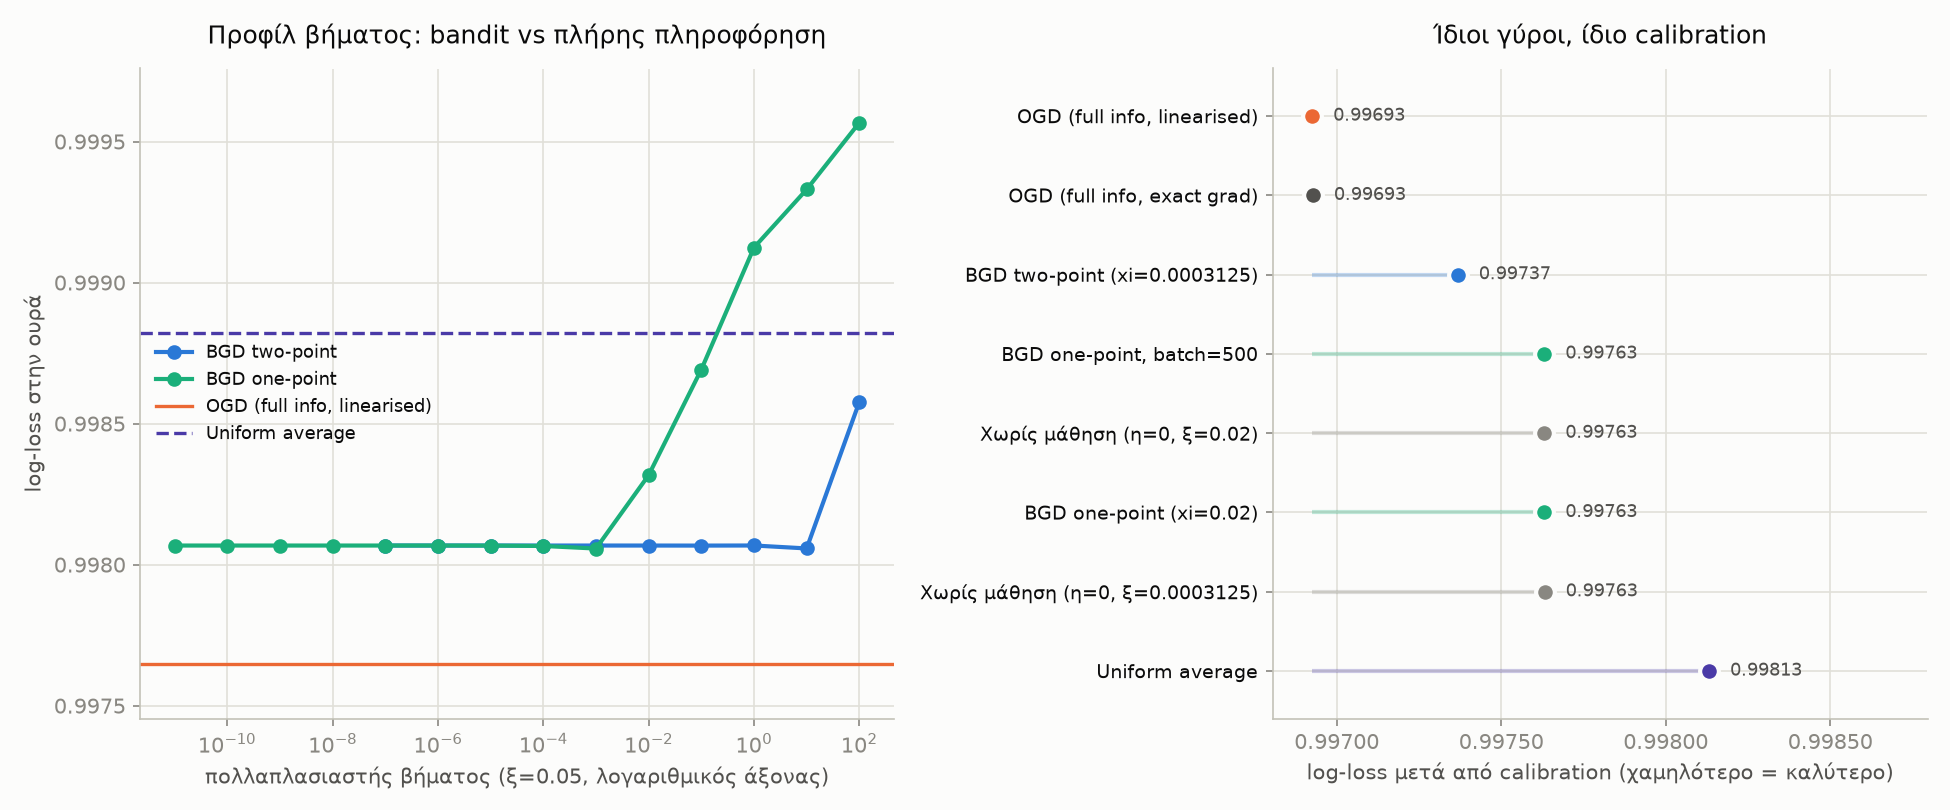
\includegraphics[width=\textwidth]{bandit_oco.png}
\caption{Left, the step profile on which the selection is made; right, the final comparison.}
\end{figure}

\paragraph{The control that makes the numbers interpretable.} The obvious reading (``BGD beats
the uniform average, so the bandit feedback taught it something'') is wrong, and this thesis
made it in a first draft before correcting it. Under the Sleeping Experts reduction the weight
vector moves even with a \emph{zero} step: every time the awake set changes, the persistent
state is reprojected onto a simplex of different dimension, and that churn alone produces
non-uniform weights. Measured directly: at $\eta=0$ the weights are as far as $0.69$ from
uniform in max norm. The correct benchmark is therefore not the uniform average but \emph{the
same algorithm with the step set to zero}: same shrinkage, same perturbations, same projection
dynamics, no learning. Whatever lies between that control and BGD is what the bandit signal
actually bought.

\begin{table}[H]
\centering
\small
\begin{tabular}{lrr}
\toprule
& \textbf{Projection without learning} & \textbf{$+$ bandit learning} \\
\midrule
Two-point BGD & $+0.000500$ \;(41.4\%) & $+0.000264$ \;(21.9\%) \\
One-point BGD & $+0.000501$ \;(41.5\%) & $\mathbf{-0.000000}$ \;(0.0\%) \\
\bottomrule
\end{tabular}
\caption{Decomposition of the full-information margin (uniform average $0.998132$ against OGD
$0.996926$, i.e. $0.001206$) into what the projection gives with no learning at all and what the
bandit feedback adds on top.}
\label{tab:bandit-decomp}
\end{table}

\paragraph{The one-point estimator learns nothing here.} Selection on train drives its step to
$1.4\cdot10^{-14}$, and the whole region from $10^{-14}$ to $9\cdot10^{-11}$ ties at the same
train score $0.998375$: this is the plateau of not learning, and the selector simply takes its
endpoint. Any positive amount of learning hurts. The cause is quantified by the alignment of a
single round's estimate with the true gradient: for the two-point estimator the mean cosine is
$+0.27$, whereas for the one-point estimator it is $+0.002$, that is zero. The signal is $0.2\%$
of the size of the estimate; summing over $T$ rounds reduces the noise by $\sqrt{T}\approx277$,
which leaves an effective ratio of about $0.55$, still below one. \textbf{The horizon is not
long enough} for a one-point estimator on a $25$-dimensional simplex.

\paragraph{The one legitimate fix was tried and changes nothing.} The variance argument dictates a
specific intervention: accumulating the estimate for $m$ rounds before stepping, which raises the
effective ratio by $\sqrt{m}$ and keeps the point in the interior of the simplex, so that the
projection does not asymmetrically clip the noise. $m$ was swept over $\{1,20,100,500\}$ across
five orders of magnitude of the step. \emph{No} combination produces an interior optimum: every
cell is either on the plateau or worse, and batching does exactly what the theory predicts (it
tolerates a larger step without damage) while never producing a gain. The signal is not there
to be amplified.

\paragraph{A caveat about the two-point estimator.} Its shrinkage parameter was driven by the
selection to the lower end of the admissible interval. This is not an accident but what is to be
expected: as $\delta\to 0$ the finite difference converges to the exact directional derivative, so
the two-point estimator \emph{ceases to be bandit}. The $21.9\%$ of Table~\ref{tab:bandit-decomp}
must therefore be read as an upper bound on what the two-query approach achieves, not as
performance in a genuine bandit environment. The one-point estimator is the honest experiment, and
its answer is zero.

\paragraph{What remains from the experiment.} Two things, and neither is what it was looking for.
First, that one-point feedback is insufficient at this horizon, with a quantitative explanation of
why and with the obvious fix tried and rejected. Second, and more useful for the rest of the
thesis, that \textbf{$41\%$ of the mixture's margin over the uniform average does not come from
learning at all}, but from the reprojection forced by the changing composition of the panel. This
is an independent finding about Sleeping Experts dynamics and it agrees with the measurement of
\S\ref{sec:res-deploy}, where weight movement in the late stages turned out to be dominated by the
projection and not by the gradient step.

\paragraph{A side finding in favour of linearisation.} The full-information control with the
\emph{exact} gradient of the non-linear loss ties with the implemented, linearised OGD
($+0.000002$, $p=0.934$). The simplification of Lemma~\ref{lem:linearization}, that is, costs
nothing measurable on these data: a confirmation of a design choice that until now rested only
on the theoretical argument that the linear problem is harder.

\subsection{Markovian switching of market regimes}
\label{sec:res-regime}

The Markov chain on the \emph{weight vector} has already been tried and rejected: every
transition kernel selects $\alpha=0$ on train, i.e. collapses to plain OGD. Here the chain runs
over a different object, over \emph{market states}. We maintain $K$ latent regimes, one weight
vector per regime under Sleeping Experts, and a belief updated by the forward recursion of a
hidden Markov model; each regime steps in proportion to its responsibility. $K=1$ reproduces
\file{run\_ogd\_sleeping} exactly.

The motivation is measured and not hypothetical: \S\ref{sec:res-panels} and the information
arrival analysis show that the closing advantage varies 26-fold depending on how much the line
moved. There is therefore a genuine latent state in the data. The regime is deliberately left
\emph{latent}, so that it can be checked afterwards whether the chain discovers it on its own.

\paragraph{The first version failed in a diagnosable way.} The mean belief stayed at exactly
$0.500$ for both regimes. The regimes \emph{never differentiated}: they receive the same loss
vector, so from a symmetric starting point they follow identical trajectories and their
likelihoods stay equal. The result was simply OGD with the step divided by $K$, and it lost
significantly ($+0.000128$, $p<0.001$). The symmetric solution is a fixed point of the dynamics,
and an explicit differentiation mechanism is required.

\paragraph{After the fix: a tie.} A belief sharpness $\beta$, a forgetting factor $\gamma$ and a
per-regime clock were added. Selection on train gives $K=3$, $\beta=30$, $\gamma=0$, $\tau=0$,
with calibrated log-loss $0.996909$ against OGD's $0.996926$: a difference of $-0.000016$,
$p=0.211$, \textbf{a tie}. The $\beta=30$ is a genuine interior optimum; the grid was extended
to $1000$ and the values $100$, $300$, $1000$ are all worse on train.

\paragraph{Two findings that nullify any claim that ``the chain works''.} First, the tail is
\emph{flat}: from $\beta=3$ to $\beta=1000$ it moves between $0.997647$ and $0.997649$, a range of
two millionths over three orders of magnitude of the parameter, while the train differences
driving the selection are ten times larger. The selection is fitting noise, exactly as in the
joint sweep of step and calibration rate (\S\ref{sec:res-negative}). Second, and more decisive,
$\tau=0$ is selected (no transition), and the standard deviation of the belief is $0.0000$: it
freezes early and never moves again. There is therefore no Markovian switching. What remains is
a fixed convex combination of three OGDs with different initialisations, that is
\emph{ensembling}, and the small point-estimate gain must be attributed to that.

\paragraph{And the chain discovers nothing.} The correlation of the belief with the measured line
movement is undefined, precisely because the belief is constant. The latent regime corresponds to
no measurable property of the market. The answer to the question the experiment posed (does a
model with no side information discover the structure that was measured directly?) is negative
and clean.

\begin{figure}[H]
\centering
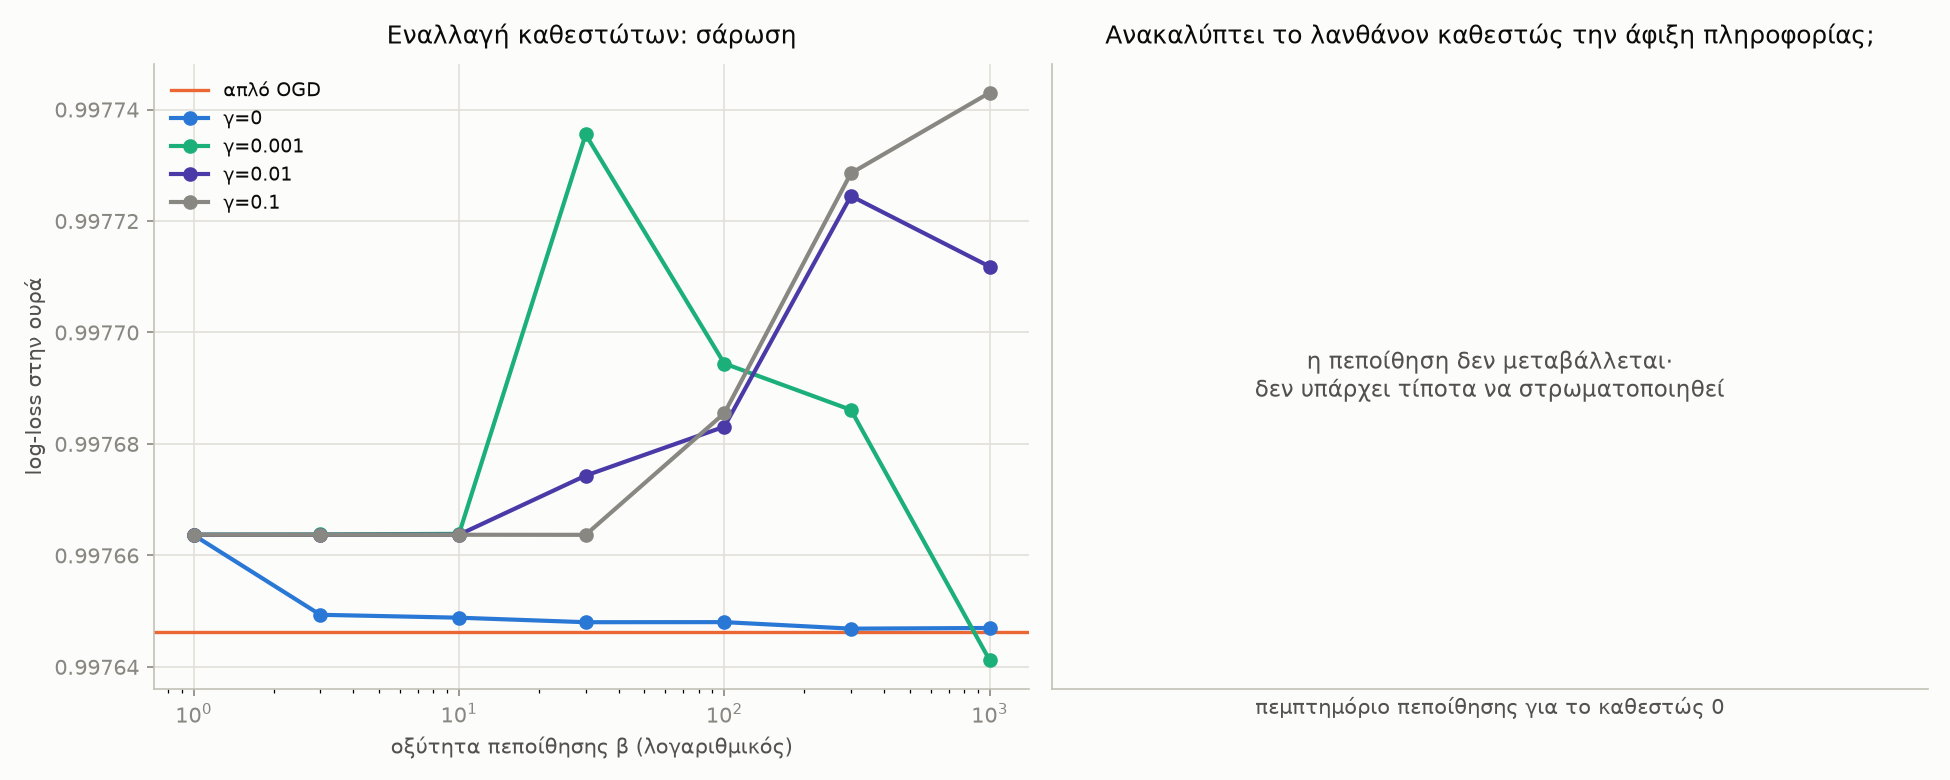
\includegraphics[width=\textwidth]{regime_switching.png}
\caption{Left, the sweep of the belief sharpness. Right, the check of whether the latent regime
corresponds to the measured information arrival.}
\end{figure}

This is the third independent instance of the strongest pattern in the thesis: once the step is
tuned, no movement of mass over the experts offers anything measurable. Fixed-Share, transition
kernels, and now regime switching. The difference here is that the failure was \emph{diagnosed}
rather than merely observed.

\section{Negative results}
\label{sec:res-negative}

A series of plausible hypotheses was tested and rejected. We report them explicitly, since each
one bounds the method's scope.

\paragraph{Per-league specialisation does not help.} A separate model per league loses to the
single model in \emph{every} one of the six leagues tested. Two plausible causes: each league has
only 2,231--3,800 matches, far too few for the online algorithm to converge on its own, and the
specialists end up trusting largely the \emph{same} experts as the unified model, i.e. they do not
discover anything local.

\paragraph{Fixed-Share does not help.} Every $\alpha > 0$ worsens the log-loss ($0.99842$ at
$\alpha=0$ against $0.99885$ and above); the $\alpha=0$ case reproduces plain Hedge exactly, which
is what makes this a statement about Fixed-Share and not about the particular implementation of
it. Sweeping $\alpha$ \emph{jointly} with the step shows why:
$\alpha$ only ever helped when the step was too large. Both control the same quantity (how fast
the algorithm forgets), and the step is the more efficient of the two instruments.

\paragraph{A per-expert step clock significantly worsens things.} Replacing the global $t$ with
the number of rounds in which each expert was awake (which is literally the quantity the
Sleeping Experts guarantee speaks about) gives a result that is \emph{better on train but
$-0.00073$ on the tail}. An expert with 6.9\% coverage receives a step about 14 times larger,
and the mixture chases the rare bookmakers, whose apparent quality is confounded with the
difficulty of the single season in which they appear. This is the clearest demonstration of
overfitting in the thesis.

\paragraph{Joint selection of step and calibration rate offers nothing.} The two parameters do not
interact: the optimal calibration rate is $0.15$ in 11 of 11 rows. Joint selection on train in fact
picks a worse value for OGD, since the grid is nearly flat there and the selection fits noise.

\paragraph{Markovian transition kernels offer nothing.} All three kernels of
\S\ref{sec:markov-theory}(a) (uniform, towards the opening/closing twin, towards the same
market phase) select $\alpha = 0$ on the chronological prefix, i.e. collapse to plain OGD. The
paired tests confirm this with a mean difference of $0.000000$ \emph{exactly} and $p=1.000$,
not approximately. The finding agrees with Fixed-Share: once the step itself is tuned, no
post-hoc movement of mass has anything left to correct, because both control the same quantity.
It is worth noting, however, that at \emph{large} $\alpha$ the structured kernels do measurably
less damage than the uniform one, i.e. the panel's structure is real and detectable, merely
redundant.

\paragraph{The Bayesian version of Kelly does not beat the fixed fraction.} The formulation of
\S\ref{sec:mcmc-theory} is theoretically more attractive, since the shrinkage emerges from the
uncertainty instead of being imposed. Paired with the fixed $\tfrac14$ over the same bets, for
four targets and two stake levels, it gives \textbf{6 ties and 2 significant losses} (PSC at both
levels, $p=0.003$ and $p=0.049$), with \emph{no} significant win. The selected concentration
parameter $\kappa$ is moreover unstable across targets with no evident pattern, an indication that
the selection is fitting noise. The most likely explanation is that the Dirichlet model does not
correctly describe the mechanism generating bookmakers' disagreements: their disagreements are not
independent noise around a common truth but systematic pricing differences, so the posterior is
the wrong distribution and the shrinkage it produces does not correspond to the real uncertainty.

\paragraph{Draws are practically unpredictable as a primary prediction.} Although they constitute
$\sim$26\% of the matches, the best algorithm selects them as the most likely outcome in $0.4\%$
of cases. This is a known phenomenon of football prediction, confirmed here quantitatively.

\section{Discussion}
\label{sec:discussion}

\subsection{What the thesis showed}

Summarising the findings of this chapter, three answers emerge at different levels.

At the level of \textbf{method}, the framework works, but less than a first reading suggests. An
online mixture of published odds, with no data beyond the prices themselves, consistently and
significantly beats both the uniform average and the overwhelming majority of individual
companies. That this is achieved with no statistical assumption about the distribution of the
data, and with predictions that are by construction out-of-sample, is the main methodological
gain of the online approach over a classical batch one. The limitation emerged from the
experiment of \S\ref{sec:res-bandit}: with an explicit zero-step control it turns out that $41\%$
of the margin over the uniform average is produced by the repeated projection onto the simplex,
that is by the geometry of the reduction and not by learning. The weighting does add something
real, but less than one would conclude by comparing it directly against the average.

At the level of \textbf{comparison with the market}, the answer is more guarded. Over the full
decade and on the full panel the sharpest bookmaker remains significantly ahead. In the
configuration finally selected the difference ceases to be significant, and in the deployment
test the mixture beats every opening price and ties with the bookmakers' closing prices. The real
limit is not a bookmaker: Betfair Exchange, which is an exchange and therefore a market price
without an operator's margin, significantly beats us. The honest statement is that we
\emph{reach} the leading edge of the bookmaker market, not that we exceed it, and that the market
without an intermediary remains ahead.

At the level of \textbf{economic exploitation}, the answer is negative. Improved log-loss does
not translate into profitability, because the quality difference gained is smaller than the
margin the market charges. This distinction (between being a better forecaster and being able
to exploit it) is, in our view, the most practically useful conclusion. The third OCO stage
does not overturn it, but it clarifies what stake size can and cannot do: the learned
multiplier multiplies the final bankroll where an edge exists and shrinks itself where none
does, without ever creating an edge. The choice of opponent remains far more important than the
choice of stake.

\subsection{When learning pays off: heterogeneity as a precondition}
\label{sec:disc-hetero}

The recurring pattern throughout the thesis is that learned weighting pays off when, and only
when, the experts differ substantially in quality. The finding appears independently at three
points:

\begin{itemize}
  \item On the full panel, which contains 13 good closing and 13 systematically worse opening
        experts, all three algorithms significantly beat the plain average.
  \item On the homogeneous panels (opening only or closing only) Hedge and FTRL \emph{lose} to
        the average, in 8 tests out of 8.
  \item Removing Pinnacle from the \emph{opening} panel, even OGD falls behind the average
        ($0.99999$ against $0.99990$) and significantly loses to VC\_BV.
\end{itemize}

The fourth case (the closing panel without Pinnacle) does \textbf{not} support the pattern any
more, and is reported for precisely that reason. There OGD ranks first ($0.99919$) with the
average second ($0.99921$). The difference is $0.00002$, practically zero, so the correct
reading is not ``weighting wins here'' but ``the two are indistinguishable'', which still
agrees with the general conclusion, since in a homogeneous panel weighting has nothing to
learn.

The interpretation is that the gain comes primarily not from the algorithm but from the structure
of the panel. When a real quality difference exists, the weighting finds and exploits it. When it
does not, the adaptation is pure cost: the algorithm pays estimation noise with no corresponding
benefit, and the average (which estimates nothing) proves more robust.

This conclusion has direct practical value for anyone who would apply the framework in another
field. The criterion for a good set of experts is not their number, nor how much their numbers
differ, but whether they are \emph{produced by different processes}.

\subsection{The character of the method}

A property of the framework deserves noting that is not always made explicit. The model is not
trained and then applied; there is no moment at which it ``knows'' and subsequently acts. At every
match it states a claim, the outcome refutes it to some degree, and the claim is revised. The
refutation \emph{is} the material of learning, literally: the gradient that updates the weights
equals the loss of the prediction against what happened. Without error nothing is learned, and the
weights at any moment are not the answer but the current state of an unresolved disagreement.

This property was also confirmed empirically, where we did not expect it. We examined whether the
mixture eventually ``settles'' somewhere and quietens down, given that the step decays as
$1/\sqrt{t}$. It does not. The step does fall by a factor of 277 from the first round to the last,
but the mean movement of the weight vector per round is $0.0353$, $0.0226$, $0.0227$, $0.0284$
over the four quarters: the last moves \emph{more} than the second and the third, at a point where
the step is two hundred and seventy times smaller. The reason is that the movement is dominated by
the projection onto the simplex every time the awake set changes, not by the step: the same
phenomenon that \S\ref{sec:res-bandit} isolates quantitatively, showing that the projection on
its own, with no learning at all, produces $41\%$ of the mixture's margin over the uniform
average.

Relatedly, the theoretically superior alternative (the Aggregating Algorithm, which exploits
the exp-concavity of the log-loss and achieves regret $\leq \ln N$ with a constant $\eta=1$)
performs in practice \emph{worse than the uniform average}. The explanation is precisely that
its bound concerns a \emph{static} comparator, while the panel is not static: Pinnacle's
coverage collapses towards the end of the period, and an algorithm that concentrates quickly on
a few experts is punished exactly by an expert that disappears.

% =====================================================================
\chapter{Conclusions and future work}
\label{ch:conclusion}
% =====================================================================

\section{Conclusions}

\begin{enumerate}
  \item \textbf{The OCO framework applies successfully to betting markets.} An online mixture of
        published odds significantly beats the uniform average and the overwhelming majority of
        individual companies, with no assumption about the distribution of the data.

  \item \textbf{The mixture reaches but does not exceed the market's leading edge.} In the
        configuration selected, the difference from the sharpest bookmaker ceases to be
        statistically significant. In the deployment test it significantly beats every opening
        price and ties with the bookmakers' closing prices. The limit is set by Betfair Exchange,
        which is not a bookmaker but an exchange, that is a market price without an operator's
        margin: that one significantly beats us.

  \item \textbf{A substantial part of the apparent superiority is not learning.} Under the
        Sleeping Experts reduction the weight vector moves even with a zero step, because the
        projection is redone onto a simplex of different dimension every time the awake set
        changes. With an explicit zero-step control, $41\%$ of the margin over the uniform average
        is attributed to this geometry and not to the algorithm. Every future comparison against
        the uniform average ought to carry the same control.

  \item \textbf{Panel heterogeneity is a precondition, not a detail.} Learned weighting pays off
        only when the experts differ substantially; on a homogeneous set the plain average is at
        least as robust. The finding is independently confirmed at three points, while at a fourth
        (the closing panel without Pinnacle) the two end up indistinguishable
        (\S\ref{sec:disc-hetero}).

  \item \textbf{Worst-case theoretical steps are not optimal in practice}, and they in fact miss in
        opposite directions per algorithm. They protect against an adversary that betting odds are
        not. The only exception is the third OCO stage, where the algorithm that exploits the
        structure of the loss accepts the theoretical constant uncorrected.

  \item \textbf{Better prediction does not mean profit.} The quality difference gained falls short
        of the market's margin, and whatever edge exists concerns specific companies, not a general
        strategy.

  \item \textbf{In the third OCO stage, \emph{what} is learned decides the outcome.} Learning the
        stake directly fails systematically, because the comparator ``best constant stake'' does
        not contain the closed form and because it throws away the probability the two preceding
        stages have just produced. Learning the \emph{multiplier} on top of the closed form ties
        with the fixed coefficient on the closing targets and significantly beats it on the opening
        ones, by 8 wins to 2 losses, discovering a different risk appetite for each opponent
        without ever being told who that opponent is. It is also the only place in the thesis where
        theory's a-priori constant came out right without correction, precisely because the
        algorithm that uses it exploits the structure of the loss.

  \item \textbf{Methodological discipline in comparisons is decisive.} Several intermediate
        ``findings'' turned out to be artefacts of comparing over different sets of matches, or of
        selection on a flat grid. The requirement of common rounds and the reporting of a held-out
        tail is what caught them. The sharpest instance concerns the step multipliers themselves:
        read off the held-out tail, two of the three appear mistuned, and the thesis carried that
        caveat for a time; read off the chronological prefix, which is what the protocol specifies,
        all three are already at their optimum. Selecting on the tail is selecting on the test set,
        and here the two criteria disagree.
\end{enumerate}

\section{The odds as a social relation}
\label{sec:disc-material}

It is easy to read the weights as abstract parameters. Each expert here is a business, with its
own costs, its own risk tolerance and its own business model, and the differences the algorithm
learns are differences between those. Pinnacle is ahead not because it necessarily has a better
prediction model but because it operates on a low margin and does not restrict winning players,
so that its price is continuously corrected by informed bettors instead of their being shut out;
in the 2025--26 window the best forecaster is not even a bookmaker but Betfair Exchange, where
the price carries no operator margin; and over ten seasons the market did \emph{not} become more
accurate (no series shows a significant trend in log-loss or ECE, $p$ from $0.21$ to $1.00$) but
it did become more expensive, the overround rising from $4.42\%$ to $6.00\%$ ($p=0.0007$).

\paragraph{The odds appear as a property of the match.} De-vigging institutionalises the
impression: you strip the margin in order to ``recover'' the true probability, as though beneath
the commercial form there were a determinate number that the house distorts and you restore.
There is none. Remove Pinnacle from the panel and the ``probability'' changes, because what was
being measured was not knowledge about football but position in the market. The technique itself
confesses as much: Shin's parameter $z$ (\S\ref{sec:microstructure-theory}) \textbf{is} the
estimated proportion of informed bettors, that is a social relation, and it enters the method as
a \emph{nuisance parameter} to be removed. This is what Marx called the fetishism of the
commodity: a definite social relation between people assumes the form of a property of a thing.
Here the relation between the house, the informed and everyone else assumes the form of a number
attached to a football match, and the fetishism operates \emph{inside} the formalism rather than
outside it.

It does not follow that there is nothing to be known. The uncertainty term of Murphy's
decomposition is improved by no method and no amount of capital, and the closing price beats the
opening price systematically. Something resists, and that something is the match, which occurs
whatever anyone prices it at. The precise statement is therefore not that the odds lack
objectivity but that \textbf{they are not objective about what they appear to be about}: there is
no probability of the match waiting to be read off, there is an objective expression of a
relation, and it is measured, compared and ranked reproducibly. The fetish is not that the number
is false but that we misattribute what it is a number of. If appearance and essence coincided
directly, Marx observed, all science would be superfluous; here the distance between them is
itself a measurement.

\paragraph{Who pays, and why the market got dearer without getting better.} The microstructure
model of \S\ref{sec:microstructure-theory} already supplies the mechanism: the market maker
charges a margin sufficient for the gains from the uninformed to cover the losses to the
informed. But ``informed'' is not a mental state; it is a position with respect to the
\textbf{material means}: data feeds, capital enough to move a line, and accounts that are not
closed when you win. That same model makes the margin an increasing function of the proportion of
informed traders, which appears at first to conflict with the measurement, since a market
increasingly exposed to informed money should also have become more accurate. The two reconcile
once it is asked \emph{how} an operator may respond to informed money. It can absorb it, letting
the price be corrected and growing more accurate, which is Pinnacle's model and the reason
Pinnacle is hardest to beat. Or it can exclude it and raise the price instead, which leaves
accuracy exactly where it was and the overround higher. A decade of rising margins with flat
accuracy is the signature of the second response, and it is why better prediction does not
convert into profit: the quality gained is measured against a toll that moves against it.

\paragraph{Profit and loss is the house's category, not ours.} For the house no question of
truth arises, only of the balance sheet, and the mechanism that secures it is not better
forecasting but control of access. The thesis measures both sides of this. The significant edge
appears against two targets only, WHC ($38.52\times$, $p<0.001$) and IW ($7.89\times$,
$p=0.008$), both recreational-facing, while against the one house that does not exclude winners
the simulation \emph{loses} significantly ($0.0002\times$, $p<0.001$). The edge exists exactly
where it cannot be exercised and is absent exactly where it could be, and the reason is the same
on both sides: the sharp house has the right price \emph{because} it lets informed money correct
it, the soft houses have the wrong one \emph{because} they drive that money away. What separates
the houses is not how well they predict but whom they let bet and at what price, which is
Levitt's (2004) observation that betting markets are organised around the bettor rather than
around the price. The odds, read this way, are not a statement about the match but \textbf{an
offer, revocable against whoever accepts it too well}. Account restrictions are not measured
here, since the data are prices and not customer outcomes; what is measured is the concentration
of the edge at the soft houses and its absence at the sharp one. The revocation itself has been
documented elsewhere: Kaunitz et al.\ (2017) bet a profitable odds-based strategy with real
money for five months and report that the response was not a correction of the prices but stake
limits and account closures directed at them as clients. That is the complement of our
measurement rather than a repetition of it, and the two together close the argument: the edge
concentrates where access is controlled, and it is withdrawn when exercised.

\paragraph{No teleology, and the path is not a straight line.} Every regret bound in the thesis
assumes the opposite: comparison against the best \textbf{fixed} weight vector, which is the same
presupposition as de-vigging, a determinate property where there is a relation in motion. The
refutation is measured. The Aggregating Algorithm, holding the strongest bound in the thesis and
one independent of the horizon, performs worse than the uniform average, because Pinnacle's
coverage collapses and whoever concentrates quickly is punished by an expert that disappears; the
schedule designed for convergence loses significantly to the non-decaying one for FTRL
($p=0.001$); and the weights move more in the final quarter than in the middle ones, at a point
where the step is orders of magnitude smaller. Nor does the thesis's own knowledge advance
linearly: nine ideas were tried and rejected, findings reverse when the window changes, and a
caveat about the step multipliers proved unfounded as soon as the selection criterion was
corrected (\S\ref{sec:res-steps}). The path moves in cycles and settles into no system; the tree
of knowledge stays green precisely because it is never finished. Characteristically, Fixed-Share,
the explicit attempt to replace the fixed comparator with a sequence, does not help, because the
movement \textbf{was already there} inside the step. The formalism was tracking motion from the
outset while declaring a static aim: the fetish was not in the equations but in what we took them
to be measuring.

That is what is at stake practically. A strictly positivist protocol would have delivered three 
wrong conclusions: that the entire margin over the uniform average is a product of learning, when $41\%$ of it is not
(\S\ref{sec:res-bandit}); that variety among the experts suffices, when on a homogeneous panel
the learned weighting loses in 8 tests out of 8 (\S\ref{sec:disc-hetero}); and that the market's
hierarchy is a matter of technical capability, when it is a matter of margin, of access, and of
who is permitted to win. All three were avoided by the same move: refusing to identify what is
measured with what is real, and looking for the explanation in the relations that produce the
measurement.

\section{Limitations}
\label{sec:limits}

The following limitations are stated explicitly.

\paragraph{Window choice is a form of selection.} Three time windows were examined and the result
improved in our favour with every narrowing. This is exactly the pattern that produces spurious
findings, and for that reason all three are reported, the less favourable alongside the
favourable.

\paragraph{Statistical power in the narrow windows.} The deployment test rests on 8,151 matches
against 71,818 for the full comparison. The confidence intervals are correspondingly wider, so a
``tie'' partly means ``less data'' and not only ``equal quality''.

\paragraph{The merging of identities is an inference.} The VC/BetVictor merge rests on
non-overlapping temporal presence, not on an official source. There may well be comparable
rebrands that were not identified.

\paragraph{The simulation ignores liquidity.} Account limits, stake restrictions and available
liquidity are not modelled: precisely the mechanisms by which companies restrict winning
players in practice. The simulation shows the \emph{statistical existence} of an edge, not
viable profitability.

\paragraph{The causality audit is not exhaustive.} One leakage channel was found and fixed in the
leave-one-out design, but there may be others at less obvious points.

\paragraph{The causal interpretations are plausible, not proved.} The explanation, for example, of
the margin increase as a commercial decision is consistent with the data but is not directly
tested by it.

\section{Future work}

\paragraph{A live odds feed.} Everything in this thesis is computed on a historical file, which
means every result is a statement about what the method \emph{would} have done. The framework
itself does not require that: the three stages are online and causal, each round costs
$O(N\log N)$, and the state is a single weight vector plus two scalars, so the whole chain runs in
real time against a streaming odds API. What such an implementation would add is not speed but the
two things a file cannot supply. First, the prices would be the ones actually available for
staking rather than the ones recorded afterwards, which is precisely the gap
\S\ref{sec:limits} identifies between a statistical and an exploitable edge: account limits,
stake caps and liquidity become observable instead of assumed away. Second, the opening/closing
distinction, which this thesis can only treat as two static snapshots, becomes the continuous
object it really is: the measurement of \S\ref{sec:res-arrival}, that the closing advantage is
concentrated in the top quintile of line movement, suggests the interesting quantity is not the
final price but the trajectory, and only a live feed records it.

\paragraph{A second sport.} Extending to basketball or tennis would show whether the framework
generalises beyond football. The cost is mainly a new data pipeline, since the algorithms do not
change. A two-outcome sport, where the structure of the problem simplifies, is of particular
interest.

\paragraph{Bayesian Model Averaging as a baseline.} A full BMA baseline would give an empirical
point of comparison against the online algorithms, and would further illuminate the failure of the
Aggregating Algorithm.

\appendix
% GENERATED FILE -- do not edit by hand.
% Produced by scripts/make_appendix_tables.py --en from results/*.csv.

\chapter{Full result tables}
\label{app:tables}

This appendix gives in full the tables that the chapters of the main text present in abridged
form. It is generated automatically from the result files, so that it cannot drift away from
them.

\section{Ranking and statistical significance}
{\scriptsize
\begin{longtable}{@{}rrrrrrrr@{}}
\caption{Full Tier-A ranking, ten seasons.}\label{app:ranking}\\
\toprule \textbf{Rounds} & \textbf{log-loss (cal.)} & \textbf{Brier (raw)} & \textbf{Brier (cal.)} & \textbf{raw\_rps} & \textbf{calibrated\_rps} & \textbf{Acc. (raw)} & \textbf{Acc.} \\\midrule\endfirsthead
\multicolumn{8}{l}{\emph{(continued)}}\\\toprule \textbf{Rounds} & \textbf{log-loss (cal.)} & \textbf{Brier (raw)} & \textbf{Brier (cal.)} & \textbf{raw\_rps} & \textbf{calibrated\_rps} & \textbf{Acc. (raw)} & \textbf{Acc.} \\\midrule\endhead
\bottomrule\endfoot
71,818 & 0.99685 & 0.59592 & 0.59577 & 0.20263 & 0.20256 & 0.50611 & 0.50611 \\
76,584 & 0.99693 & 0.59612 & 0.59586 & 0.20270 & 0.20257 & 0.50662 & 0.50662 \\
76,584 & 0.99773 & 0.59674 & 0.59637 & 0.20297 & 0.20278 & 0.50649 & 0.50649 \\
76,584 & 0.99774 & 0.59674 & 0.59638 & 0.20297 & 0.20279 & 0.50653 & 0.50653 \\
76,584 & 0.99813 & 0.59703 & 0.59665 & 0.20311 & 0.20291 & 0.50593 & 0.50593 \\
53,267 & 0.99910 & 0.59732 & 0.59711 & 0.20314 & 0.20301 & 0.50705 & 0.50705 \\
49,755 & 0.99919 & 0.59769 & 0.59728 & 0.20316 & 0.20293 & 0.50624 & 0.50624 \\
68,397 & 1.0003 & 0.59833 & 0.59806 & 0.20372 & 0.20359 & 0.50355 & 0.50355 \\
65,470 & 1.0005 & 0.59860 & 0.59818 & 0.20387 & 0.20368 & 0.50309 & 0.50309 \\
71,284 & 1.0005 & 0.59838 & 0.59824 & 0.20376 & 0.20369 & 0.50309 & 0.50309 \\
57,185 & 1.0006 & 0.59899 & 0.59826 & 0.20412 & 0.20379 & 0.50214 & 0.50214 \\
72,752 & 1.0007 & 0.59873 & 0.59833 & 0.20381 & 0.20360 & 0.50355 & 0.50355 \\
76,438 & 1.0007 & 0.59852 & 0.59832 & 0.20373 & 0.20362 & 0.50377 & 0.50377 \\
\end{longtable}
}

{\scriptsize
\begin{longtable}{@{}rlrrrrrr@{}}
\caption{Every series in the panel, with no coverage threshold.}\label{app:allseries}\\
\toprule \textbf{n\_seasons\_active} & \textbf{single\_season} & \textbf{hedge\_weight\_last\_awake} & \textbf{Rounds} & \textbf{log-loss} & \textbf{Brier} & \textbf{RPS} & \textbf{Acc.} \\\midrule\endfirsthead
\multicolumn{8}{l}{\emph{(continued)}}\\\toprule \textbf{n\_seasons\_active} & \textbf{single\_season} & \textbf{hedge\_weight\_last\_awake} & \textbf{Rounds} & \textbf{log-loss} & \textbf{Brier} & \textbf{RPS} & \textbf{Acc.} \\\midrule\endhead
\bottomrule\endfoot
10 & no & 0.00000 & 71,818 & 0.99714 & 0.59592 & 0.20263 & 0.50611 \\
1 & yes & 0.16631 & 7,680 & 0.99730 & 0.59594 & 0.20251 & 0.51029 \\
10 & no & --- & 76,584 & 0.99745 & 0.59612 & 0.20270 & 0.50662 \\
2 & no & 0.04504 & 14,885 & 0.99783 & 0.59656 & 0.20253 & 0.50890 \\
1 & yes & 0.16620 & 7,681 & 0.99786 & 0.59605 & 0.20253 & 0.50814 \\
3 & no & 0.00005 & 20,972 & 0.99797 & 0.59682 & 0.20303 & 0.50644 \\
1 & yes & 0.14584 & 5,587 & 0.99819 & 0.59667 & 0.20317 & 0.50743 \\
10 & no & --- & 76,584 & 0.99842 & 0.59674 & 0.20297 & 0.50649 \\
10 & no & --- & 76,584 & 0.99843 & 0.59674 & 0.20297 & 0.50653 \\
10 & no & --- & 76,584 & 0.99886 & 0.59703 & 0.20311 & 0.50593 \\
1 & yes & 0.15156 & 5,257 & 0.99906 & 0.59732 & 0.20323 & 0.50409 \\
7 & no & 0.00009 & 53,267 & 0.99953 & 0.59732 & 0.20314 & 0.50705 \\
1 & yes & 0.11580 & 7,508 & 0.99955 & 0.59776 & 0.20303 & 0.50759 \\
6 & no & 0.00024 & 45,424 & 0.99973 & 0.59757 & 0.20326 & 0.50590 \\
7 & no & 0.00014 & 49,755 & 0.99998 & 0.59769 & 0.20316 & 0.50624 \\
6 & no & 0.00043 & 42,366 & 1.0002 & 0.59787 & 0.20349 & 0.50555 \\
1 & yes & 0.16597 & 7,673 & 1.0004 & 0.59809 & 0.20354 & 0.50541 \\
9 & no & 0.00000 & 68,397 & 1.0007 & 0.59833 & 0.20372 & 0.50355 \\
10 & no & 0.00000 & 71,284 & 1.0008 & 0.59838 & 0.20376 & 0.50309 \\
1 & yes & 0.11542 & 7,524 & 1.0009 & 0.59874 & 0.20326 & 0.50704 \\
5 & no & 0.18974 & 34,038 & 1.0009 & 0.59820 & 0.20376 & 0.50385 \\
10 & no & 0.00000 & 76,438 & 1.0011 & 0.59852 & 0.20373 & 0.50377 \\
9 & no & 0.00000 & 65,470 & 1.0012 & 0.59860 & 0.20387 & 0.50309 \\
10 & no & 0.00000 & 72,752 & 1.0014 & 0.59873 & 0.20381 & 0.50355 \\
8 & no & 0.00001 & 57,185 & 1.0019 & 0.59899 & 0.20412 & 0.50214 \\
1 & yes & 0.11836 & 7,309 & 1.0021 & 0.59938 & 0.20381 & 0.50581 \\
1 & yes & 0.16922 & 7,505 & 1.0027 & 0.59958 & 0.20402 & 0.50393 \\
1 & yes & 0.11393 & 7,619 & 1.0027 & 0.59991 & 0.20390 & 0.50532 \\
1 & yes & 0.14862 & 5,393 & 1.0044 & 0.60099 & 0.20444 & 0.50028 \\
2 & no & 0.04495 & 14,763 & 1.0072 & 0.60309 & 0.20526 & 0.49604 \\
\end{longtable}
}

{\footnotesize
\begin{longtable}{@{}lrrrrr@{}}
\caption{The full battery of significance tests.}\label{app:sig}\\
\toprule \textbf{Comparison} & \textbf{$n$} & \textbf{Mean diff.} & \textbf{CI low} & \textbf{CI high} & \textbf{$p$} \\\midrule\endfirsthead
\multicolumn{6}{l}{\emph{(continued)}}\\\toprule \textbf{Comparison} & \textbf{$n$} & \textbf{Mean diff.} & \textbf{CI low} & \textbf{CI high} & \textbf{$p$} \\\midrule\endhead
\bottomrule\endfoot
OGD vs PSC (raw) & 71,818 & 0.00065 & 0.00044 & 0.00086 & 0.00000 \\
OGD vs PSC (calibrated) & 71,818 & 0.00043 & 0.00020 & 0.00064 & 0.00000 \\
OGD vs B365C (raw) & 53,267 & -0.00063 & -0.00093 & -0.00034 & 0.00000 \\
OGD vs Hedge (raw) & 76,584 & -0.00097 & -0.00118 & -0.00075 & 0.00000 \\
OGD vs FTRL (raw) & 76,584 & -0.00098 & -0.00120 & -0.00077 & 0.00000 \\
OGD vs Uniform average (raw) & 76,584 & -0.00141 & -0.00167 & -0.00115 & 0.00000 \\
Hedge vs Uniform average (raw) & 76,584 & -0.00044 & -0.00062 & -0.00026 & 0.00000 \\
FTRL vs Uniform average (raw) & 76,584 & -0.00043 & -0.00061 & -0.00025 & 0.00000 \\
Hedge: raw vs calibrated & 76,584 & 0.00069 & 0.00040 & 0.00096 & 0.00000 \\
OGD: raw vs calibrated & 76,584 & 0.00053 & 0.00027 & 0.00078 & 0.00000 \\
FTRL: raw vs calibrated & 76,584 & 0.00069 & 0.00040 & 0.00096 & 0.00000 \\
Uniform average: raw vs calibrated & 76,584 & 0.00073 & 0.00044 & 0.00101 & 0.00000 \\
\end{longtable}
}

\section{Panel and de-vig method}
{\scriptsize
\begin{longtable}{@{}llrrrrrrl@{}}
\caption{Panel $\times$ algorithm --- proportional normalisation.}\label{app:opening_vs_cΑναλ}\\
\toprule \textbf{Panel} & \textbf{Algorithm} & \textbf{n\_bookmakers} & \textbf{Rounds} & \textbf{log-loss} & \textbf{Brier} & \textbf{RPS} & \textbf{Acc.} & \textbf{De-vig} \\\midrule\endfirsthead
\multicolumn{9}{l}{\emph{(continued)}}\\\toprule \textbf{Panel} & \textbf{Algorithm} & \textbf{n\_bookmakers} & \textbf{Rounds} & \textbf{log-loss} & \textbf{Brier} & \textbf{RPS} & \textbf{Acc.} & \textbf{De-vig} \\\midrule\endhead
\bottomrule\endfoot
closing & FTRL & 13 & 76,521 & 0.99761 & 0.59621 & 0.20272 & 0.50658 & Basic \\
full & FTRL & 26 & 76,584 & 0.99843 & 0.59674 & 0.20297 & 0.50653 & Basic \\
opening & FTRL & 13 & 76,557 & 1.0009 & 0.59842 & 0.20375 & 0.50394 & Basic \\
closing & Hedge & 13 & 76,521 & 0.99762 & 0.59622 & 0.20272 & 0.50659 & Basic \\
full & Hedge & 26 & 76,584 & 0.99842 & 0.59674 & 0.20297 & 0.50649 & Basic \\
opening & Hedge & 13 & 76,557 & 1.0009 & 0.59842 & 0.20375 & 0.50402 & Basic \\
closing & OGD & 13 & 76,521 & 0.99722 & 0.59598 & 0.20263 & 0.50648 & Basic \\
full & OGD & 26 & 76,584 & 0.99745 & 0.59612 & 0.20270 & 0.50662 & Basic \\
opening & OGD & 13 & 76,557 & 1.0008 & 0.59832 & 0.20370 & 0.50391 & Basic \\
closing & Uniform average & 13 & 76,521 & 0.99748 & 0.59612 & 0.20269 & 0.50672 & Basic \\
full & Uniform average & 26 & 76,584 & 0.99886 & 0.59703 & 0.20311 & 0.50593 & Basic \\
opening & Uniform average & 13 & 76,557 & 1.0008 & 0.59836 & 0.20373 & 0.50398 & Basic \\
\end{longtable}
}

{\scriptsize
\begin{longtable}{@{}llrrrrrrl@{}}
\caption{Panel $\times$ algorithm --- Shin normalisation.}\label{app:opening_vs_cΚανο}\\
\toprule \textbf{Panel} & \textbf{Algorithm} & \textbf{n\_bookmakers} & \textbf{Rounds} & \textbf{log-loss} & \textbf{Brier} & \textbf{RPS} & \textbf{Acc.} & \textbf{De-vig} \\\midrule\endfirsthead
\multicolumn{9}{l}{\emph{(continued)}}\\\toprule \textbf{Panel} & \textbf{Algorithm} & \textbf{n\_bookmakers} & \textbf{Rounds} & \textbf{log-loss} & \textbf{Brier} & \textbf{RPS} & \textbf{Acc.} & \textbf{De-vig} \\\midrule\endhead
\bottomrule\endfoot
closing & FTRL & 13 & 76,521 & 0.99714 & 0.59596 & 0.20260 & 0.50659 & Shin \\
full & FTRL & 26 & 76,584 & 0.99782 & 0.59642 & 0.20282 & 0.50646 & Shin \\
opening & FTRL & 13 & 76,557 & 1.0003 & 0.59812 & 0.20361 & 0.50385 & Shin \\
closing & Hedge & 13 & 76,521 & 0.99714 & 0.59596 & 0.20260 & 0.50659 & Shin \\
full & Hedge & 26 & 76,584 & 0.99781 & 0.59641 & 0.20282 & 0.50645 & Shin \\
opening & Hedge & 13 & 76,557 & 1.0003 & 0.59812 & 0.20361 & 0.50387 & Shin \\
closing & OGD & 13 & 76,521 & 0.99689 & 0.59581 & 0.20255 & 0.50658 & Shin \\
full & OGD & 26 & 76,584 & 0.99709 & 0.59595 & 0.20262 & 0.50682 & Shin \\
opening & OGD & 13 & 76,557 & 1.0002 & 0.59804 & 0.20357 & 0.50389 & Shin \\
closing & Uniform average & 13 & 76,521 & 0.99703 & 0.59589 & 0.20258 & 0.50674 & Shin \\
full & Uniform average & 26 & 76,584 & 0.99824 & 0.59670 & 0.20295 & 0.50598 & Shin \\
opening & Uniform average & 13 & 76,557 & 1.0002 & 0.59805 & 0.20358 & 0.50393 & Shin \\
\end{longtable}
}

{\scriptsize
\begin{longtable}{@{}llllrlrrrr@{}}
\caption{Each algorithm against the plain average, proportional.}\label{app:vsuniαναλ}\\
\toprule \textbf{Panel} & \textbf{Algorithm} & \textbf{Metric} & \textbf{lower\_is\_better} & \textbf{$n$} & \textbf{De-vig} & \textbf{Mean diff.} & \textbf{CI low} & \textbf{CI high} & \textbf{$p$} \\\midrule\endfirsthead
\multicolumn{10}{l}{\emph{(continued)}}\\\toprule \textbf{Panel} & \textbf{Algorithm} & \textbf{Metric} & \textbf{lower\_is\_better} & \textbf{$n$} & \textbf{De-vig} & \textbf{Mean diff.} & \textbf{CI low} & \textbf{CI high} & \textbf{$p$} \\\midrule\endhead
\bottomrule\endfoot
opening & Hedge & log\_loss & yes & 76,557 & Basic & 0.00008 & 0.00001 & 0.00014 & 0.01900 \\
opening & Hedge & brier & yes & 76,557 & Basic & 0.00006 & 0.00002 & 0.00009 & 0.00000 \\
opening & Hedge & accuracy & no & 76,557 & Basic & 0.00004 & -0.00021 & 0.00027 & 0.81700 \\
opening & OGD & log\_loss & yes & 76,557 & Basic & -0.00004 & -0.00013 & 0.00006 & 0.43300 \\
opening & OGD & brier & yes & 76,557 & Basic & -0.00004 & -0.00010 & 0.00001 & 0.14000 \\
opening & OGD & accuracy & no & 76,557 & Basic & -0.00007 & -0.00043 & 0.00033 & 0.75900 \\
opening & FTRL & log\_loss & yes & 76,557 & Basic & 0.00008 & 0.00002 & 0.00014 & 0.01500 \\
opening & FTRL & brier & yes & 76,557 & Basic & 0.00006 & 0.00002 & 0.00010 & 0.00200 \\
opening & FTRL & accuracy & no & 76,557 & Basic & -0.00004 & -0.00027 & 0.00020 & 0.78200 \\
closing & Hedge & log\_loss & yes & 76,521 & Basic & 0.00014 & 0.00010 & 0.00018 & 0.00000 \\
closing & Hedge & brier & yes & 76,521 & Basic & 0.00009 & 0.00007 & 0.00012 & 0.00000 \\
closing & Hedge & accuracy & no & 76,521 & Basic & -0.00013 & -0.00046 & 0.00018 & 0.42300 \\
closing & OGD & log\_loss & yes & 76,521 & Basic & -0.00026 & -0.00036 & -0.00016 & 0.00000 \\
closing & OGD & brier & yes & 76,521 & Basic & -0.00014 & -0.00021 & -0.00008 & 0.00000 \\
closing & OGD & accuracy & no & 76,521 & Basic & -0.00025 & -0.00071 & 0.00022 & 0.29700 \\
closing & FTRL & log\_loss & yes & 76,521 & Basic & 0.00013 & 0.00009 & 0.00018 & 0.00000 \\
closing & FTRL & brier & yes & 76,521 & Basic & 0.00009 & 0.00006 & 0.00012 & 0.00000 \\
closing & FTRL & accuracy & no & 76,521 & Basic & -0.00014 & -0.00046 & 0.00017 & 0.36700 \\
full & Hedge & log\_loss & yes & 76,584 & Basic & -0.00044 & -0.00062 & -0.00026 & 0.00000 \\
full & Hedge & brier & yes & 76,584 & Basic & -0.00030 & -0.00042 & -0.00017 & 0.00000 \\
full & Hedge & accuracy & no & 76,584 & Basic & 0.00056 & -0.00014 & 0.00125 & 0.12300 \\
full & OGD & log\_loss & yes & 76,584 & Basic & -0.00141 & -0.00167 & -0.00115 & 0.00000 \\
full & OGD & brier & yes & 76,584 & Basic & -0.00091 & -0.00108 & -0.00074 & 0.00000 \\
full & OGD & accuracy & no & 76,584 & Basic & 0.00069 & -0.00025 & 0.00162 & 0.15600 \\
full & FTRL & log\_loss & yes & 76,584 & Basic & -0.00043 & -0.00061 & -0.00025 & 0.00000 \\
full & FTRL & brier & yes & 76,584 & Basic & -0.00029 & -0.00041 & -0.00017 & 0.00000 \\
full & FTRL & accuracy & no & 76,584 & Basic & 0.00060 & -0.00010 & 0.00131 & 0.10800 \\
\end{longtable}
}

{\scriptsize
\begin{longtable}{@{}llllrlrrrr@{}}
\caption{Each algorithm against the plain average, Shin.}\label{app:vsuniShin}\\
\toprule \textbf{Panel} & \textbf{Algorithm} & \textbf{Metric} & \textbf{lower\_is\_better} & \textbf{$n$} & \textbf{De-vig} & \textbf{Mean diff.} & \textbf{CI low} & \textbf{CI high} & \textbf{$p$} \\\midrule\endfirsthead
\multicolumn{10}{l}{\emph{(continued)}}\\\toprule \textbf{Panel} & \textbf{Algorithm} & \textbf{Metric} & \textbf{lower\_is\_better} & \textbf{$n$} & \textbf{De-vig} & \textbf{Mean diff.} & \textbf{CI low} & \textbf{CI high} & \textbf{$p$} \\\midrule\endhead
\bottomrule\endfoot
opening & Hedge & log\_loss & yes & 76,557 & Shin & 0.00011 & 0.00004 & 0.00018 & 0.00000 \\
opening & Hedge & brier & yes & 76,557 & Shin & 0.00008 & 0.00003 & 0.00012 & 0.00000 \\
opening & Hedge & accuracy & no & 76,557 & Shin & -0.00005 & -0.00029 & 0.00018 & 0.69700 \\
opening & OGD & log\_loss & yes & 76,557 & Shin & 0.00002 & -0.00008 & 0.00013 & 0.73600 \\
opening & OGD & brier & yes & 76,557 & Shin & -0.00001 & -0.00006 & 0.00005 & 0.82600 \\
opening & OGD & accuracy & no & 76,557 & Shin & -0.00004 & -0.00042 & 0.00035 & 0.89600 \\
opening & FTRL & log\_loss & yes & 76,557 & Shin & 0.00011 & 0.00004 & 0.00019 & 0.00000 \\
opening & FTRL & brier & yes & 76,557 & Shin & 0.00008 & 0.00003 & 0.00012 & 0.00000 \\
opening & FTRL & accuracy & no & 76,557 & Shin & -0.00008 & -0.00033 & 0.00017 & 0.55900 \\
closing & Hedge & log\_loss & yes & 76,521 & Shin & 0.00011 & 0.00007 & 0.00016 & 0.00000 \\
closing & Hedge & brier & yes & 76,521 & Shin & 0.00008 & 0.00005 & 0.00010 & 0.00000 \\
closing & Hedge & accuracy & no & 76,521 & Shin & -0.00014 & -0.00046 & 0.00017 & 0.37900 \\
closing & OGD & log\_loss & yes & 76,521 & Shin & -0.00014 & -0.00023 & -0.00004 & 0.00500 \\
closing & OGD & brier & yes & 76,521 & Shin & -0.00007 & -0.00013 & -0.00001 & 0.01600 \\
closing & OGD & accuracy & no & 76,521 & Shin & -0.00016 & -0.00060 & 0.00029 & 0.51300 \\
closing & FTRL & log\_loss & yes & 76,521 & Shin & 0.00011 & 0.00006 & 0.00015 & 0.00000 \\
closing & FTRL & brier & yes & 76,521 & Shin & 0.00007 & 0.00004 & 0.00010 & 0.00000 \\
closing & FTRL & accuracy & no & 76,521 & Shin & -0.00014 & -0.00046 & 0.00017 & 0.37900 \\
full & Hedge & log\_loss & yes & 76,584 & Shin & -0.00043 & -0.00062 & -0.00023 & 0.00000 \\
full & Hedge & brier & yes & 76,584 & Shin & -0.00029 & -0.00042 & -0.00016 & 0.00000 \\
full & Hedge & accuracy & no & 76,584 & Shin & 0.00047 & -0.00025 & 0.00116 & 0.21900 \\
full & OGD & log\_loss & yes & 76,584 & Shin & -0.00115 & -0.00140 & -0.00090 & 0.00000 \\
full & OGD & brier & yes & 76,584 & Shin & -0.00075 & -0.00092 & -0.00059 & 0.00000 \\
full & OGD & accuracy & no & 76,584 & Shin & 0.00084 & -0.00010 & 0.00175 & 0.07900 \\
full & FTRL & log\_loss & yes & 76,584 & Shin & -0.00042 & -0.00061 & -0.00023 & 0.00000 \\
full & FTRL & brier & yes & 76,584 & Shin & -0.00028 & -0.00041 & -0.00015 & 0.00000 \\
full & FTRL & accuracy & no & 76,584 & Shin & 0.00048 & -0.00024 & 0.00118 & 0.20300 \\
\end{longtable}
}

\section{Configurations}
{\small
\begin{longtable}{@{}llrrr@{}}
\caption{Stacking of configurations.}\label{app:cfg}\\
\toprule \textbf{Config.} & \textbf{Stage} & \textbf{full\_log\_loss} & \textbf{train} & \textbf{tail} \\\midrule\endfirsthead
\multicolumn{5}{l}{\emph{(continued)}}\\\toprule \textbf{Config.} & \textbf{Stage} & \textbf{full\_log\_loss} & \textbf{train} & \textbf{tail} \\\midrule\endhead
\bottomrule\endfoot
baseline (full 26, basic) & raw & 0.99779 & 0.99860 & 0.99536 \\
baseline (full 26, basic) & calibrated & 0.99728 & 0.99801 & 0.99508 \\
closing only, basic & raw & 0.99733 & 0.99801 & 0.99528 \\
closing only, basic & calibrated & 0.99693 & 0.99756 & 0.99506 \\
full 26, Shin & raw & 0.99745 & 0.99822 & 0.99512 \\
full 26, Shin & calibrated & 0.99731 & 0.99804 & 0.99512 \\
A: closing + Shin & raw & 0.99702 & 0.99767 & 0.99506 \\
A: closing + Shin & calibrated & 0.99692 & 0.99754 & 0.99507 \\
B: A minus single-season & raw & 0.99702 & 0.99767 & 0.99509 \\
B: A minus single-season & calibrated & 0.99692 & 0.99754 & 0.99509 \\
PSC alone & raw & 0.99714 & 0.99776 & 0.99526 \\
PSC alone & calibrated & 0.99685 & 0.99746 & 0.99502 \\
\end{longtable}
}

{\footnotesize
\begin{longtable}{@{}llrrrrr@{}}
\caption{Paired tests of configurations.}\label{app:cfgsig}\\
\toprule \textbf{Stage} & \textbf{Against} & \textbf{$n$} & \textbf{Mean diff.} & \textbf{CI low} & \textbf{CI high} & \textbf{$p$} \\\midrule\endfirsthead
\multicolumn{7}{l}{\emph{(continued)}}\\\toprule \textbf{Stage} & \textbf{Against} & \textbf{$n$} & \textbf{Mean diff.} & \textbf{CI low} & \textbf{CI high} & \textbf{$p$} \\\midrule\endhead
\bottomrule\endfoot
raw & PSC alone & 71,818 & 0.00065 & 0.00044 & 0.00086 & 0.00000 \\
calibrated & PSC alone & 71,818 & 0.00043 & 0.00020 & 0.00064 & 0.00000 \\
raw & PSC alone & 71,818 & 0.00019 & 0.00009 & 0.00029 & 0.00000 \\
raw & baseline (full 26, basic) & 71,818 & -0.00046 & -0.00064 & -0.00029 & 0.00000 \\
calibrated & PSC alone & 71,818 & 0.00009 & -0.00003 & 0.00020 & 0.14300 \\
calibrated & baseline (full 26, basic) & 71,818 & -0.00034 & -0.00053 & -0.00016 & 0.00000 \\
raw & PSC alone & 71,818 & 0.00031 & 0.00008 & 0.00054 & 0.01100 \\
raw & baseline (full 26, basic) & 71,818 & -0.00034 & -0.00046 & -0.00022 & 0.00000 \\
calibrated & PSC alone & 71,818 & 0.00046 & 0.00021 & 0.00069 & 0.00000 \\
calibrated & baseline (full 26, basic) & 71,818 & 0.00004 & -0.00002 & 0.00009 & 0.18100 \\
raw & PSC alone & 71,818 & -0.00012 & -0.00025 & 0.00000 & 0.05700 \\
raw & baseline (full 26, basic) & 71,818 & -0.00077 & -0.00100 & -0.00056 & 0.00000 \\
calibrated & PSC alone & 71,818 & 0.00007 & -0.00004 & 0.00018 & 0.23400 \\
calibrated & baseline (full 26, basic) & 71,818 & -0.00036 & -0.00056 & -0.00016 & 0.00000 \\
raw & PSC alone & 71,818 & -0.00011 & -0.00024 & 0.00001 & 0.07200 \\
raw & baseline (full 26, basic) & 71,818 & -0.00077 & -0.00099 & -0.00055 & 0.00000 \\
calibrated & PSC alone & 71,818 & 0.00008 & -0.00003 & 0.00018 & 0.18100 \\
calibrated & baseline (full 26, basic) & 71,818 & -0.00035 & -0.00055 & -0.00015 & 0.00000 \\
\end{longtable}
}

\section{Without Pinnacle}
{\scriptsize
\begin{longtable}{@{}rllrrrrr@{}}
\caption{Ranking without Pinnacle, three panels.}\label{app:np}\\
\toprule \textbf{rank} & \textbf{Series} & \textbf{Type} & \textbf{Coverage \%} & \textbf{log-loss (raw)} & \textbf{log-loss (cal.)} & \textbf{train} & \textbf{tail} \\\midrule\endfirsthead
\multicolumn{8}{l}{\emph{(continued)}}\\\toprule \textbf{rank} & \textbf{Series} & \textbf{Type} & \textbf{Coverage \%} & \textbf{log-loss (raw)} & \textbf{log-loss (cal.)} & \textbf{train} & \textbf{tail} \\\midrule\endhead
\bottomrule\endfoot
1 & FTRL & algorithm & 100.0000 & 0.99854 & 0.99771 & 1.0011 & 0.98747 \\
2 & Hedge & algorithm & 100.0000 & 0.99854 & 0.99771 & 1.0011 & 0.98747 \\
3 & OGD & algorithm & 100.0000 & 0.99858 & 0.99782 & 1.0013 & 0.98735 \\
4 & Uniform average & algorithm & 100.0000 & 0.99927 & 0.99837 & 1.0016 & 0.98862 \\
5 & VC\_BV & bookmaker & 89.3098 & 1.0004 & 0.99987 & 1.0028 & 0.99113 \\
6 & WH & bookmaker & 85.4878 & 1.0012 & 1.0003 & 1.0031 & 0.99191 \\
7 & BW & bookmaker & 94.9963 & 1.0011 & 1.0004 & 1.0032 & 0.99187 \\
8 & B365 & bookmaker & 99.8094 & 1.0008 & 1.0004 & 1.0033 & 0.99173 \\
9 & IW & bookmaker & 74.6696 & 1.0017 & 1.0005 & 1.0035 & 0.99146 \\
1 & OGD & algorithm & 69.5916 & 0.99997 & 0.99919 & 1.0041 & 0.98459 \\
2 & Uniform average & algorithm & 69.5916 & 1.0000 & 0.99921 & 1.0041 & 0.98462 \\
3 & FTRL & algorithm & 69.5916 & 1.0000 & 0.99921 & 1.0041 & 0.98463 \\
4 & Hedge & algorithm & 69.5916 & 1.0000 & 0.99921 & 1.0041 & 0.98463 \\
5 & VC\_BVC & bookmaker & 59.3127 & 0.99981 & 0.99929 & 1.0043 & 0.98426 \\
6 & B365C & bookmaker & 69.5537 & 1.0001 & 0.99955 & 1.0044 & 0.98493 \\
7 & IWC & bookmaker & 44.4453 & 1.0007 & 0.99957 & 1.0042 & 0.98558 \\
8 & BWC & bookmaker & 64.9679 & 1.0005 & 0.99968 & 1.0047 & 0.98463 \\
9 & WHC & bookmaker & 55.3196 & 1.0008 & 1.0002 & 1.0050 & 0.98579 \\
1 & VC\_BV & bookmaker & 89.3098 & 1.0004 & 0.99987 & 1.0028 & 0.99113 \\
2 & Uniform average & algorithm & 99.9647 & 1.0007 & 0.99990 & 1.0028 & 0.99130 \\
3 & FTRL & algorithm & 99.9647 & 1.0007 & 0.99991 & 1.0028 & 0.99131 \\
4 & Hedge & algorithm & 99.9647 & 1.0007 & 0.99991 & 1.0028 & 0.99131 \\
5 & OGD & algorithm & 99.9647 & 1.0007 & 0.99999 & 1.0029 & 0.99136 \\
6 & WH & bookmaker & 85.4878 & 1.0012 & 1.0003 & 1.0031 & 0.99191 \\
7 & BW & bookmaker & 94.9963 & 1.0011 & 1.0004 & 1.0032 & 0.99187 \\
8 & B365 & bookmaker & 99.8094 & 1.0008 & 1.0004 & 1.0033 & 0.99173 \\
9 & IW & bookmaker & 74.6696 & 1.0017 & 1.0005 & 1.0035 & 0.99146 \\
\end{longtable}
}

{\footnotesize
\begin{longtable}{@{}lrlrrrr@{}}
\caption{Paired tests without Pinnacle.}\label{app:npsig}\\
\toprule \textbf{Bookmaker} & \textbf{$n$} & \textbf{Verdict} & \textbf{Mean diff.} & \textbf{CI low} & \textbf{CI high} & \textbf{$p$} \\\midrule\endfirsthead
\multicolumn{7}{l}{\emph{(continued)}}\\\toprule \textbf{Bookmaker} & \textbf{$n$} & \textbf{Verdict} & \textbf{Mean diff.} & \textbf{CI low} & \textbf{CI high} & \textbf{$p$} \\\midrule\endhead
\bottomrule\endfoot
IW & 54,877 & OGD better & -0.00315 & -0.00366 & -0.00262 & 0.00000 \\
WH & 54,877 & OGD better & -0.00259 & -0.00311 & -0.00208 & 0.00000 \\
BW & 54,877 & OGD better & -0.00255 & -0.00309 & -0.00205 & 0.00000 \\
B365 & 54,877 & OGD better & -0.00223 & -0.00273 & -0.00176 & 0.00000 \\
VC\_BV & 54,877 & OGD better & -0.00181 & -0.00230 & -0.00134 & 0.00000 \\
WHC & 32,210 & OGD better & -0.00088 & -0.00135 & -0.00039 & 0.00000 \\
IWC & 32,210 & OGD better & -0.00077 & -0.00108 & -0.00047 & 0.00000 \\
BWC & 32,210 & OGD better & -0.00051 & -0.00085 & -0.00017 & 0.00700 \\
B365C & 32,210 & tie (not significant) & -0.00011 & -0.00040 & 0.00021 & 0.50500 \\
VC\_BVC & 32,210 & tie (not significant) & 0.00016 & -0.00015 & 0.00043 & 0.28400 \\
IW & 54,877 & OGD better & -0.00105 & -0.00130 & -0.00076 & 0.00000 \\
WH & 54,877 & OGD better & -0.00048 & -0.00074 & -0.00019 & 0.00200 \\
BW & 54,877 & OGD better & -0.00045 & -0.00070 & -0.00020 & 0.00000 \\
B365 & 54,877 & tie (not significant) & -0.00012 & -0.00033 & 0.00007 & 0.20300 \\
VC\_BV & 54,877 & VC\_BV better & 0.00030 & 0.00009 & 0.00050 & 0.00400 \\
\end{longtable}
}

\section{Recent window and deployment test}
{\scriptsize
\begin{longtable}{@{}lrrrrrrr@{}}
\caption{Ranking, five seasons.}\label{app:rw}\\
\toprule \textbf{Phase} & \textbf{Coverage \%} & \textbf{Rounds} & \textbf{log-loss (raw)} & \textbf{log-loss (cal.)} & \textbf{Brier (raw)} & \textbf{Brier (cal.)} & \textbf{Acc.} \\\midrule\endfirsthead
\multicolumn{8}{l}{\emph{(continued)}}\\\toprule \textbf{Phase} & \textbf{Coverage \%} & \textbf{Rounds} & \textbf{log-loss (raw)} & \textbf{log-loss (cal.)} & \textbf{Brier (raw)} & \textbf{Brier (cal.)} & \textbf{Acc.} \\\midrule\endhead
\bottomrule\endfoot
closing & 87.9119 & 34,065 & 0.99471 & 0.99439 & 0.59424 & 0.59410 & 0.50976 \\
--- & 100.0000 & 38,749 & 0.99556 & 0.99495 & 0.59482 & 0.59452 & 0.51090 \\
closing & 79.6975 & 30,882 & 0.99554 & 0.99498 & 0.59483 & 0.59456 & 0.50955 \\
closing & 72.1361 & 27,952 & 0.99575 & 0.99502 & 0.59490 & 0.59450 & 0.51009 \\
closing & 91.9353 & 35,624 & 0.99609 & 0.99504 & 0.59513 & 0.59460 & 0.51039 \\
closing & 99.9974 & 38,748 & 0.99602 & 0.99543 & 0.59500 & 0.59471 & 0.51107 \\
--- & 100.0000 & 38,749 & 0.99677 & 0.99591 & 0.59559 & 0.59516 & 0.50920 \\
--- & 100.0000 & 38,749 & 0.99689 & 0.99604 & 0.59567 & 0.59524 & 0.50956 \\
--- & 100.0000 & 38,749 & 0.99692 & 0.99607 & 0.59569 & 0.59526 & 0.50954 \\
opening & 71.9090 & 27,864 & 0.99848 & 0.99771 & 0.59677 & 0.59634 & 0.50660 \\
opening & 87.6952 & 33,981 & 0.99831 & 0.99794 & 0.59665 & 0.59649 & 0.50552 \\
opening & 79.0833 & 30,644 & 0.99870 & 0.99801 & 0.59696 & 0.59660 & 0.50702 \\
opening & 91.5327 & 35,468 & 0.99981 & 0.99885 & 0.59765 & 0.59716 & 0.50665 \\
opening & 99.8400 & 38,687 & 0.99951 & 0.99896 & 0.59736 & 0.59709 & 0.50660 \\
\end{longtable}
}

{\footnotesize
\begin{longtable}{@{}lrrrrr@{}}
\caption{Significance tests, five seasons.}\label{app:rwsig}\\
\toprule \textbf{Comparison} & \textbf{$n$} & \textbf{Mean diff.} & \textbf{CI low} & \textbf{CI high} & \textbf{$p$} \\\midrule\endfirsthead
\multicolumn{6}{l}{\emph{(continued)}}\\\toprule \textbf{Comparison} & \textbf{$n$} & \textbf{Mean diff.} & \textbf{CI low} & \textbf{CI high} & \textbf{$p$} \\\midrule\endhead
\bottomrule\endfoot
OGD vs PSC (raw) & 34,065 & 0.00065 & 0.00037 & 0.00097 & 0.00000 \\
OGD vs PSC (calibrated) & 34,065 & 0.00036 & 0.00008 & 0.00067 & 0.01400 \\
OGD vs B365C (raw) & 38,748 & -0.00047 & -0.00086 & -0.00012 & 0.01400 \\
OGD vs Hedge (raw) & 38,749 & -0.00133 & -0.00166 & -0.00102 & 0.00000 \\
OGD vs FTRL (raw) & 38,749 & -0.00136 & -0.00169 & -0.00104 & 0.00000 \\
OGD vs Uniform average (raw) & 38,749 & -0.00121 & -0.00151 & -0.00092 & 0.00000 \\
Hedge vs Uniform average (raw) & 38,749 & 0.00012 & 0.00004 & 0.00019 & 0.00600 \\
FTRL vs Uniform average (raw) & 38,749 & 0.00015 & 0.00006 & 0.00023 & 0.00200 \\
Hedge: raw vs calibrated & 38,749 & 0.00085 & 0.00036 & 0.00133 & 0.00100 \\
OGD: raw vs calibrated & 38,749 & 0.00061 & 0.00021 & 0.00100 & 0.00100 \\
FTRL: raw vs calibrated & 38,749 & 0.00086 & 0.00037 & 0.00134 & 0.00100 \\
Uniform average: raw vs calibrated & 38,749 & 0.00086 & 0.00036 & 0.00135 & 0.00100 \\
\end{longtable}
}

{\scriptsize
\begin{longtable}{@{}rlrrlrrrrr@{}}
\caption{The market in the tail, five seasons.}\label{app:rwlive}\\
\toprule \textbf{rank} & \textbf{Phase} & \textbf{Coverage \%} & \textbf{log-loss} & \textbf{Bookmaker} & \textbf{$n$} & \textbf{Mean diff.} & \textbf{CI low} & \textbf{CI high} & \textbf{$p$} \\\midrule\endfirsthead
\multicolumn{10}{l}{\emph{(continued)}}\\\toprule \textbf{rank} & \textbf{Phase} & \textbf{Coverage \%} & \textbf{log-loss} & \textbf{Bookmaker} & \textbf{$n$} & \textbf{Mean diff.} & \textbf{CI low} & \textbf{CI high} & \textbf{$p$} \\\midrule\endhead
\bottomrule\endfoot
1.0000 & --- & 100.0000 & 1.0001 & --- & --- & --- & --- & --- & --- \\
2.0000 & closing & 85.0674 & 1.0002 & --- & --- & --- & --- & --- & --- \\
3.0000 & closing & 77.7447 & 1.0003 & --- & --- & --- & --- & --- & --- \\
4.0000 & closing & 75.5458 & 1.0003 & --- & --- & --- & --- & --- & --- \\
5.0000 & closing & 100.0000 & 1.0007 & --- & --- & --- & --- & --- & --- \\
6.0000 & --- & 100.0000 & 1.0008 & --- & --- & --- & --- & --- & --- \\
7.0000 & --- & 100.0000 & 1.0009 & --- & --- & --- & --- & --- & --- \\
8.0000 & --- & 100.0000 & 1.0009 & --- & --- & --- & --- & --- & --- \\
9.0000 & opening & 75.2847 & 1.0026 & --- & --- & --- & --- & --- & --- \\
10.0000 & opening & 99.8485 & 1.0030 & --- & --- & --- & --- & --- & --- \\
11.0000 & opening & 84.7697 & 1.0032 & --- & --- & --- & --- & --- & --- \\
12.0000 & opening & 77.1075 & 1.0081 & --- & --- & --- & --- & --- & --- \\
--- & opening & --- & --- & BFE & 7,699 & -0.00796 & -0.01093 & -0.00527 & 0.00000 \\
--- & opening & --- & --- & BW & 7,699 & -0.00306 & -0.00479 & -0.00141 & 0.00100 \\
--- & opening & --- & --- & B365 & 7,699 & -0.00283 & -0.00454 & -0.00118 & 0.00100 \\
--- & opening & --- & --- & PS & 7,699 & -0.00244 & -0.00406 & -0.00094 & 0.00200 \\
--- & closing & --- & --- & B365C & 7,699 & -0.00057 & -0.00146 & 0.00031 & 0.20500 \\
--- & closing & --- & --- & PSC & 7,699 & -0.00015 & -0.00056 & 0.00029 & 0.50300 \\
--- & closing & --- & --- & BFEC & 7,699 & -0.00013 & -0.00092 & 0.00074 & 0.79700 \\
--- & closing & --- & --- & BWC & 7,699 & -0.00009 & -0.00082 & 0.00064 & 0.81500 \\
\end{longtable}
}

{\small
\begin{longtable}{@{}rllrr@{}}
\caption{Deployment test 2025--26.}\label{app:dep}\\
\toprule \textbf{rank} & \textbf{Series} & \textbf{Type} & \textbf{Coverage \%} & \textbf{log-loss} \\\midrule\endfirsthead
\multicolumn{5}{l}{\emph{(continued)}}\\\toprule \textbf{rank} & \textbf{Series} & \textbf{Type} & \textbf{Coverage \%} & \textbf{log-loss} \\\midrule\endhead
\bottomrule\endfoot
1 & BFEC & closing & 96.1811 & 1.0004 \\
2 & OGD closing-only, online & αλγόριθμος & 100.0000 & 1.0011 \\
3 & OGD πλήρες panel, online & αλγόριθμος & 100.0000 & 1.0013 \\
4 & BWC & closing & 75.5400 & 1.0015 \\
5 & OGD closing-only, παγωμένο & αλγόριθμος & 100.0000 & 1.0015 \\
6 & B365C & closing & 100.0000 & 1.0017 \\
7 & OGD πλήρες panel, παγωμένο & αλγόριθμος & 100.0000 & 1.0018 \\
8 & B365 & opening & 99.7840 & 1.0037 \\
9 & BW & opening & 75.1253 & 1.0042 \\
10 & BFE & opening & 95.3171 & 1.0076 \\
\end{longtable}
}

{\footnotesize
\begin{longtable}{@{}llrlrrrr@{}}
\caption{Paired tests, deployment 2025--26.}\label{app:depsig}\\
\toprule \textbf{Bookmaker} & \textbf{Phase} & \textbf{$n$} & \textbf{Verdict} & \textbf{Mean diff.} & \textbf{CI low} & \textbf{CI high} & \textbf{$p$} \\\midrule\endfirsthead
\multicolumn{8}{l}{\emph{(continued)}}\\\toprule \textbf{Bookmaker} & \textbf{Phase} & \textbf{$n$} & \textbf{Verdict} & \textbf{Mean diff.} & \textbf{CI low} & \textbf{CI high} & \textbf{$p$} \\\midrule\endhead
\bottomrule\endfoot
B365 & opening & 8,151 & αλγόριθμος & -0.00241 & -0.00382 & -0.00102 & 0.00100 \\
B365C & closing & 8,151 & ισοπαλία & -0.00036 & -0.00121 & 0.00054 & 0.39000 \\
BFE & opening & 8,151 & αλγόριθμος & -0.00629 & -0.00878 & -0.00386 & 0.00000 \\
BFEC & closing & 8,151 & BFEC & 0.00089 & 0.00016 & 0.00166 & 0.01300 \\
BW & opening & 8,151 & αλγόριθμος & -0.00287 & -0.00431 & -0.00141 & 0.00000 \\
BWC & closing & 8,151 & ισοπαλία & -0.00017 & -0.00087 & 0.00058 & 0.68500 \\
PS & opening & 6,857 & αλγόριθμος & -0.00228 & -0.00408 & -0.00058 & 0.00700 \\
PSC & closing & 6,892 & ισοπαλία & -0.00013 & -0.00058 & 0.00030 & 0.56800 \\
B365 & opening & 8,151 & αλγόριθμος & -0.00188 & -0.00313 & -0.00066 & 0.00500 \\
B365C & closing & 8,151 & ισοπαλία & 0.00018 & -0.00080 & 0.00122 & 0.75100 \\
BFE & opening & 8,151 & αλγόριθμος & -0.00575 & -0.00821 & -0.00337 & 0.00000 \\
BFEC & closing & 8,151 & BFEC & 0.00143 & 0.00046 & 0.00238 & 0.00200 \\
BW & opening & 8,151 & αλγόριθμος & -0.00233 & -0.00358 & -0.00112 & 0.00000 \\
BWC & closing & 8,151 & ισοπαλία & 0.00037 & -0.00043 & 0.00123 & 0.34200 \\
PS & opening & 6,857 & αλγόριθμος & -0.00219 & -0.00407 & -0.00042 & 0.01500 \\
PSC & closing & 6,892 & ισοπαλία & -0.00004 & -0.00038 & 0.00030 & 0.79600 \\
B365 & opening & 8,151 & αλγόριθμος & -0.00260 & -0.00417 & -0.00106 & 0.00200 \\
B365C & closing & 8,151 & ισοπαλία & -0.00055 & -0.00137 & 0.00030 & 0.19300 \\
BFE & opening & 8,151 & αλγόριθμος & -0.00647 & -0.00904 & -0.00389 & 0.00000 \\
BFEC & closing & 8,151 & ισοπαλία & 0.00070 & -0.00000 & 0.00138 & 0.05200 \\
BW & opening & 8,151 & αλγόριθμος & -0.00306 & -0.00466 & -0.00140 & 0.00100 \\
BWC & closing & 8,151 & ισοπαλία & -0.00036 & -0.00107 & 0.00042 & 0.36100 \\
PS & opening & 6,857 & αλγόριθμος & -0.00223 & -0.00418 & -0.00036 & 0.01900 \\
PSC & closing & 6,892 & ισοπαλία & -0.00009 & -0.00038 & 0.00021 & 0.53200 \\
B365 & opening & 8,151 & αλγόριθμος & -0.00220 & -0.00374 & -0.00068 & 0.00700 \\
B365C & closing & 8,151 & ισοπαλία & -0.00014 & -0.00097 & 0.00076 & 0.71400 \\
BFE & opening & 8,151 & αλγόριθμος & -0.00607 & -0.00860 & -0.00353 & 0.00000 \\
BFEC & closing & 8,151 & BFEC & 0.00111 & 0.00028 & 0.00192 & 0.00300 \\
BW & opening & 8,151 & αλγόριθμος & -0.00265 & -0.00419 & -0.00110 & 0.00000 \\
BWC & closing & 8,151 & ισοπαλία & 0.00005 & -0.00061 & 0.00076 & 0.85000 \\
PS & opening & 6,857 & αλγόριθμος & -0.00223 & -0.00422 & -0.00035 & 0.01900 \\
PSC & closing & 6,892 & ισοπαλία & -0.00009 & -0.00031 & 0.00013 & 0.44400 \\
\end{longtable}
}

\section{Value betting}
{\scriptsize
\begin{longtable}{@{}lllllrrrrr@{}}
\caption{Full sweep of training panel $\times$ target $\times$ normalisation.}\label{app:vbsweep}\\
\toprule \textbf{De-vig} & \textbf{Train panel} & \textbf{Phase} & \textbf{Bookmaker} & \textbf{Stage} & \textbf{Bets} & \textbf{log-growth} & \textbf{CI low} & \textbf{CI high} & \textbf{$p$} \\\midrule\endfirsthead
\multicolumn{10}{l}{\emph{(continued)}}\\\toprule \textbf{De-vig} & \textbf{Train panel} & \textbf{Phase} & \textbf{Bookmaker} & \textbf{Stage} & \textbf{Bets} & \textbf{log-growth} & \textbf{CI low} & \textbf{CI high} & \textbf{$p$} \\\midrule\endhead
\bottomrule\endfoot
Basic & closing-trained & closing & PSC & raw & 20,580 & -0.00012 & -0.00019 & -0.00005 & 0.00100 \\
Basic & closing-trained & closing & PSC & calibrated & 19,497 & -0.00003 & -0.00010 & 0.00004 & 0.36800 \\
Basic & closing-trained & closing & B365C & raw & 7,941 & 0.00000 & -0.00012 & 0.00012 & 0.99100 \\
Basic & closing-trained & closing & B365C & calibrated & 7,643 & 0.00001 & -0.00013 & 0.00014 & 0.96800 \\
Basic & closing-trained & closing & BWC & raw & 3,134 & 0.00022 & -0.00004 & 0.00049 & 0.09100 \\
Basic & closing-trained & closing & BWC & calibrated & 6,920 & 0.00016 & 0.00001 & 0.00033 & 0.04200 \\
Basic & closing-trained & closing & VC\_BVC & raw & 5,142 & 0.00000 & -0.00015 & 0.00018 & 0.93600 \\
Basic & closing-trained & closing & VC\_BVC & calibrated & 4,561 & 0.00010 & -0.00010 & 0.00030 & 0.33900 \\
Basic & closing-trained & closing & WHC & raw & 6,633 & 0.00055 & 0.00026 & 0.00082 & 0.00000 \\
Basic & closing-trained & closing & WHC & calibrated & 7,253 & 0.00061 & 0.00028 & 0.00088 & 0.00000 \\
Basic & mixed-trained & opening & B365 & raw & 34,022 & 0.00060 & 0.00046 & 0.00072 & 0.00000 \\
Basic & mixed-trained & opening & B365 & calibrated & 35,894 & 0.00072 & 0.00057 & 0.00086 & 0.00000 \\
Basic & mixed-trained & opening & BW & raw & 24,313 & 0.00074 & 0.00060 & 0.00090 & 0.00000 \\
Basic & mixed-trained & opening & BW & calibrated & 29,845 & 0.00082 & 0.00066 & 0.00098 & 0.00000 \\
Basic & mixed-trained & closing & PSC & raw & 42,881 & -0.00028 & -0.00038 & -0.00019 & 0.00000 \\
Basic & mixed-trained & closing & PSC & calibrated & 39,997 & -0.00021 & -0.00033 & -0.00009 & 0.00000 \\
Basic & mixed-trained & opening & PS & raw & 45,926 & 0.00053 & 0.00042 & 0.00064 & 0.00000 \\
Basic & mixed-trained & opening & PS & calibrated & 48,919 & 0.00068 & 0.00056 & 0.00080 & 0.00000 \\
Basic & mixed-trained & opening & VC\_BV & raw & 25,631 & 0.00061 & 0.00046 & 0.00075 & 0.00000 \\
Basic & mixed-trained & opening & VC\_BV & calibrated & 29,112 & 0.00072 & 0.00057 & 0.00087 & 0.00000 \\
Basic & mixed-trained & opening & WH & raw & 22,036 & 0.00071 & 0.00055 & 0.00088 & 0.00000 \\
Basic & mixed-trained & opening & WH & calibrated & 27,493 & 0.00077 & 0.00061 & 0.00094 & 0.00000 \\
Basic & mixed-trained & opening & IW & raw & 16,562 & 0.00088 & 0.00070 & 0.00108 & 0.00000 \\
Basic & mixed-trained & opening & IW & calibrated & 21,808 & 0.00096 & 0.00076 & 0.00117 & 0.00000 \\
Basic & mixed-trained & closing & B365C & raw & 9,570 & -0.00011 & -0.00023 & 0.00002 & 0.09300 \\
Basic & mixed-trained & closing & B365C & calibrated & 7,970 & -0.00007 & -0.00020 & 0.00008 & 0.32800 \\
Basic & mixed-trained & closing & BWC & raw & 3,694 & 0.00008 & -0.00014 & 0.00032 & 0.52000 \\
Basic & mixed-trained & closing & BWC & calibrated & 6,607 & 0.00009 & -0.00006 & 0.00024 & 0.24700 \\
Basic & mixed-trained & closing & VC\_BVC & raw & 6,521 & -0.00012 & -0.00025 & 0.00003 & 0.10600 \\
Basic & mixed-trained & closing & VC\_BVC & calibrated & 4,653 & -0.00006 & -0.00025 & 0.00012 & 0.45500 \\
Basic & mixed-trained & closing & WHC & raw & 6,852 & 0.00044 & 0.00016 & 0.00068 & 0.00000 \\
Basic & mixed-trained & closing & WHC & calibrated & 6,565 & 0.00056 & 0.00027 & 0.00083 & 0.00000 \\
Basic & opening-trained & opening & B365 & raw & 15,836 & -0.00009 & -0.00017 & -0.00001 & 0.04100 \\
Basic & opening-trained & opening & B365 & calibrated & 10,829 & -0.00008 & -0.00017 & 0.00001 & 0.10100 \\
Basic & opening-trained & opening & BW & raw & 4,611 & -0.00008 & -0.00021 & 0.00006 & 0.24800 \\
Basic & opening-trained & opening & BW & calibrated & 7,841 & 0.00001 & -0.00010 & 0.00011 & 0.82000 \\
Basic & opening-trained & closing & PSC & raw & 57,078 & -0.00049 & -0.00061 & -0.00036 & 0.00000 \\
Basic & opening-trained & closing & PSC & calibrated & 56,645 & -0.00044 & -0.00057 & -0.00031 & 0.00000 \\
Basic & opening-trained & opening & PS & raw & 29,835 & -0.00012 & -0.00018 & -0.00007 & 0.00000 \\
Basic & opening-trained & opening & PS & calibrated & 26,675 & -0.00005 & -0.00010 & 0.00000 & 0.05500 \\
Basic & opening-trained & opening & VC\_BV & raw & 9,508 & -0.00015 & -0.00026 & -0.00005 & 0.00700 \\
Basic & opening-trained & opening & VC\_BV & calibrated & 8,083 & -0.00006 & -0.00018 & 0.00005 & 0.24500 \\
Basic & opening-trained & opening & WH & raw & 5,793 & -0.00007 & -0.00024 & 0.00010 & 0.42500 \\
Basic & opening-trained & opening & WH & calibrated & 5,931 & 0.00005 & -0.00012 & 0.00024 & 0.54500 \\
Basic & opening-trained & opening & IW & raw & 3,101 & 0.00042 & 0.00015 & 0.00067 & 0.00400 \\
Basic & opening-trained & opening & IW & calibrated & 7,443 & 0.00028 & 0.00006 & 0.00048 & 0.00800 \\
Basic & opening-trained & closing & B365C & raw & 27,138 & -0.00066 & -0.00084 & -0.00049 & 0.00000 \\
Basic & opening-trained & closing & B365C & calibrated & 27,203 & -0.00061 & -0.00079 & -0.00042 & 0.00000 \\
Basic & opening-trained & closing & BWC & raw & 19,475 & -0.00075 & -0.00094 & -0.00058 & 0.00000 \\
Basic & opening-trained & closing & BWC & calibrated & 20,931 & -0.00071 & -0.00092 & -0.00051 & 0.00000 \\
Basic & opening-trained & closing & VC\_BVC & raw & 22,741 & -0.00066 & -0.00085 & -0.00046 & 0.00000 \\
Basic & opening-trained & closing & VC\_BVC & calibrated & 22,708 & -0.00061 & -0.00082 & -0.00041 & 0.00000 \\
Basic & opening-trained & closing & WHC & raw & 16,306 & -0.00067 & -0.00087 & -0.00045 & 0.00000 \\
Basic & opening-trained & closing & WHC & calibrated & 16,588 & -0.00065 & -0.00086 & -0.00042 & 0.00000 \\
Shin & closing-trained & closing & PSC & raw & 13,136 & 0.00000 & -0.00008 & 0.00008 & 0.94700 \\
Shin & closing-trained & closing & PSC & calibrated & 18,398 & -0.00000 & -0.00008 & 0.00007 & 0.97400 \\
Shin & closing-trained & closing & B365C & raw & 5,198 & 0.00007 & -0.00008 & 0.00022 & 0.42000 \\
Shin & closing-trained & closing & B365C & calibrated & 7,374 & 0.00003 & -0.00010 & 0.00016 & 0.68700 \\
Shin & closing-trained & closing & BWC & raw & 2,535 & 0.00039 & 0.00008 & 0.00074 & 0.01400 \\
Shin & closing-trained & closing & BWC & calibrated & 6,511 & 0.00018 & 0.00002 & 0.00036 & 0.02900 \\
Shin & closing-trained & closing & VC\_BVC & raw & 2,900 & 0.00016 & -0.00009 & 0.00042 & 0.20400 \\
Shin & closing-trained & closing & VC\_BVC & calibrated & 4,097 & 0.00013 & -0.00008 & 0.00036 & 0.24500 \\
Shin & closing-trained & closing & WHC & raw & 4,980 & 0.00083 & 0.00042 & 0.00117 & 0.00100 \\
Shin & closing-trained & closing & WHC & calibrated & 6,675 & 0.00065 & 0.00032 & 0.00095 & 0.00000 \\
Shin & mixed-trained & opening & B365 & raw & 31,621 & 0.00068 & 0.00055 & 0.00081 & 0.00000 \\
Shin & mixed-trained & opening & B365 & calibrated & 34,959 & 0.00070 & 0.00056 & 0.00084 & 0.00000 \\
Shin & mixed-trained & opening & BW & raw & 23,893 & 0.00083 & 0.00068 & 0.00099 & 0.00000 \\
Shin & mixed-trained & opening & BW & calibrated & 28,919 & 0.00083 & 0.00067 & 0.00099 & 0.00000 \\
Shin & mixed-trained & closing & PSC & raw & 35,750 & -0.00024 & -0.00035 & -0.00013 & 0.00000 \\
Shin & mixed-trained & closing & PSC & calibrated & 39,367 & -0.00021 & -0.00032 & -0.00009 & 0.00000 \\
Shin & mixed-trained & opening & PS & raw & 44,003 & 0.00062 & 0.00051 & 0.00073 & 0.00000 \\
Shin & mixed-trained & opening & PS & calibrated & 48,190 & 0.00066 & 0.00054 & 0.00078 & 0.00000 \\
Shin & mixed-trained & opening & VC\_BV & raw & 23,908 & 0.00073 & 0.00057 & 0.00088 & 0.00000 \\
Shin & mixed-trained & opening & VC\_BV & calibrated & 28,218 & 0.00072 & 0.00056 & 0.00086 & 0.00000 \\
Shin & mixed-trained & opening & WH & raw & 21,430 & 0.00080 & 0.00063 & 0.00098 & 0.00000 \\
Shin & mixed-trained & opening & WH & calibrated & 26,564 & 0.00075 & 0.00059 & 0.00093 & 0.00000 \\
Shin & mixed-trained & opening & IW & raw & 17,465 & 0.00094 & 0.00074 & 0.00112 & 0.00000 \\
Shin & mixed-trained & opening & IW & calibrated & 21,369 & 0.00096 & 0.00076 & 0.00114 & 0.00000 \\
Shin & mixed-trained & closing & B365C & raw & 6,413 & -0.00008 & -0.00023 & 0.00006 & 0.25300 \\
Shin & mixed-trained & closing & B365C & calibrated & 7,786 & -0.00005 & -0.00019 & 0.00009 & 0.46700 \\
Shin & mixed-trained & closing & BWC & raw & 2,740 & 0.00016 & -0.00012 & 0.00046 & 0.28100 \\
Shin & mixed-trained & closing & BWC & calibrated & 6,132 & 0.00013 & -0.00003 & 0.00031 & 0.12000 \\
Shin & mixed-trained & closing & VC\_BVC & raw & 3,871 & -0.00010 & -0.00029 & 0.00010 & 0.30000 \\
Shin & mixed-trained & closing & VC\_BVC & calibrated & 4,216 & -0.00003 & -0.00023 & 0.00016 & 0.66800 \\
Shin & mixed-trained & closing & WHC & raw & 4,774 & 0.00073 & 0.00037 & 0.00105 & 0.00100 \\
Shin & mixed-trained & closing & WHC & calibrated & 5,914 & 0.00059 & 0.00028 & 0.00089 & 0.00000 \\
Shin & opening-trained & opening & B365 & raw & 8,796 & -0.00008 & -0.00017 & 0.00003 & 0.18800 \\
Shin & opening-trained & opening & B365 & calibrated & 10,578 & -0.00010 & -0.00019 & -0.00000 & 0.04900 \\
Shin & opening-trained & opening & BW & raw & 2,315 & 0.00006 & -0.00011 & 0.00029 & 0.40000 \\
Shin & opening-trained & opening & BW & calibrated & 7,441 & 0.00004 & -0.00007 & 0.00015 & 0.44200 \\
Shin & opening-trained & closing & PSC & raw & 55,765 & -0.00046 & -0.00058 & -0.00033 & 0.00000 \\
Shin & opening-trained & closing & PSC & calibrated & 56,441 & -0.00044 & -0.00057 & -0.00030 & 0.00000 \\
Shin & opening-trained & opening & PS & raw & 18,357 & -0.00006 & -0.00011 & -0.00000 & 0.03800 \\
Shin & opening-trained & opening & PS & calibrated & 24,953 & -0.00006 & -0.00011 & 0.00000 & 0.05400 \\
Shin & opening-trained & opening & VC\_BV & raw & 4,268 & -0.00002 & -0.00015 & 0.00012 & 0.72200 \\
Shin & opening-trained & opening & VC\_BV & calibrated & 7,333 & -0.00006 & -0.00018 & 0.00005 & 0.26500 \\
Shin & opening-trained & opening & WH & raw & 2,996 & 0.00020 & -0.00007 & 0.00051 & 0.15500 \\
Shin & opening-trained & opening & WH & calibrated & 6,418 & 0.00002 & -0.00014 & 0.00021 & 0.73700 \\
Shin & opening-trained & opening & IW & raw & 3,579 & 0.00048 & 0.00020 & 0.00074 & 0.00000 \\
Shin & opening-trained & opening & IW & calibrated & 7,179 & 0.00032 & 0.00011 & 0.00052 & 0.00100 \\
Shin & opening-trained & closing & B365C & raw & 26,159 & -0.00063 & -0.00081 & -0.00045 & 0.00000 \\
Shin & opening-trained & closing & B365C & calibrated & 27,097 & -0.00061 & -0.00081 & -0.00042 & 0.00000 \\
Shin & opening-trained & closing & BWC & raw & 19,224 & -0.00074 & -0.00093 & -0.00055 & 0.00000 \\
Shin & opening-trained & closing & BWC & calibrated & 20,970 & -0.00071 & -0.00091 & -0.00051 & 0.00000 \\
Shin & opening-trained & closing & VC\_BVC & raw & 21,857 & -0.00064 & -0.00084 & -0.00043 & 0.00000 \\
Shin & opening-trained & closing & VC\_BVC & calibrated & 22,573 & -0.00061 & -0.00081 & -0.00041 & 0.00000 \\
Shin & opening-trained & closing & WHC & raw & 15,400 & -0.00066 & -0.00088 & -0.00044 & 0.00000 \\
Shin & opening-trained & closing & WHC & calibrated & 16,333 & -0.00064 & -0.00086 & -0.00041 & 0.00000 \\
\end{longtable}
}

{\footnotesize
\begin{longtable}{@{}llrrrrrr@{}}
\caption{Sweep over all bookmakers.}\label{app:vball}\\
\toprule \textbf{Bookmaker} & \textbf{Stage} & \textbf{Bets} & \textbf{Bankroll} & \textbf{log-growth} & \textbf{CI low} & \textbf{CI high} & \textbf{$p$} \\\midrule\endfirsthead
\multicolumn{8}{l}{\emph{(continued)}}\\\toprule \textbf{Bookmaker} & \textbf{Stage} & \textbf{Bets} & \textbf{Bankroll} & \textbf{log-growth} & \textbf{CI low} & \textbf{CI high} & \textbf{$p$} \\\midrule\endhead
\bottomrule\endfoot
B365 & raw & 15,836 & 0.24472 & -0.00009 & -0.00017 & -0.00001 & 0.04100 \\
B365 & calibrated & 10,829 & 0.41079 & -0.00008 & -0.00017 & 0.00001 & 0.10100 \\
BW & raw & 4,611 & 0.67602 & -0.00008 & -0.00021 & 0.00006 & 0.24800 \\
BW & calibrated & 7,841 & 1.0913 & 0.00001 & -0.00010 & 0.00011 & 0.82000 \\
PSC & raw & 42,881 & 0.00000 & -0.00028 & -0.00038 & -0.00019 & 0.00000 \\
PSC & calibrated & 39,997 & 0.00021 & -0.00021 & -0.00033 & -0.00009 & 0.00000 \\
PS & raw & 29,835 & 0.02460 & -0.00012 & -0.00018 & -0.00007 & 0.00000 \\
PS & calibrated & 26,675 & 0.26030 & -0.00005 & -0.00010 & 0.00000 & 0.05500 \\
VC\_BV & raw & 9,508 & 0.23716 & -0.00015 & -0.00026 & -0.00005 & 0.00700 \\
VC\_BV & calibrated & 8,083 & 0.59737 & -0.00006 & -0.00018 & 0.00005 & 0.24500 \\
WH & raw & 5,793 & 0.68312 & -0.00007 & -0.00024 & 0.00010 & 0.42500 \\
WH & calibrated & 5,931 & 1.3757 & 0.00005 & -0.00012 & 0.00024 & 0.54500 \\
IW & raw & 3,101 & 3.7046 & 0.00042 & 0.00015 & 0.00067 & 0.00400 \\
IW & calibrated & 7,443 & 7.8901 & 0.00028 & 0.00006 & 0.00048 & 0.00800 \\
B365C & raw & 9,570 & 0.36496 & -0.00011 & -0.00023 & 0.00002 & 0.09300 \\
B365C & calibrated & 7,970 & 0.58286 & -0.00007 & -0.00020 & 0.00008 & 0.32800 \\
BWC & raw & 3,694 & 1.3448 & 0.00008 & -0.00014 & 0.00032 & 0.52000 \\
BWC & calibrated & 6,607 & 1.8050 & 0.00009 & -0.00006 & 0.00024 & 0.24700 \\
VC\_BVC & raw & 6,521 & 0.46013 & -0.00012 & -0.00025 & 0.00003 & 0.10600 \\
VC\_BVC & calibrated & 4,653 & 0.75253 & -0.00006 & -0.00025 & 0.00012 & 0.45500 \\
WHC & raw & 6,852 & 19.7908 & 0.00044 & 0.00016 & 0.00068 & 0.00000 \\
WHC & calibrated & 6,565 & 38.5182 & 0.00056 & 0.00027 & 0.00083 & 0.00000 \\
\end{longtable}
}

{\footnotesize
\begin{longtable}{@{}lllrrrrrr@{}}
\caption{Value betting, five seasons.}\label{app:vbrw}\\
\toprule \textbf{Bookmaker} & \textbf{Phase} & \textbf{Stage} & \textbf{Bets} & \textbf{Bankroll} & \textbf{log-growth} & \textbf{CI low} & \textbf{CI high} & \textbf{$p$} \\\midrule\endfirsthead
\multicolumn{9}{l}{\emph{(continued)}}\\\toprule \textbf{Bookmaker} & \textbf{Phase} & \textbf{Stage} & \textbf{Bets} & \textbf{Bankroll} & \textbf{log-growth} & \textbf{CI low} & \textbf{CI high} & \textbf{$p$} \\\midrule\endhead
\bottomrule\endfoot
B365 & opening & raw & 5,183 & 0.68039 & -0.00007 & -0.00023 & 0.00005 & 0.21600 \\
B365 & opening & calibrated & 4,493 & 0.61559 & -0.00011 & -0.00028 & 0.00005 & 0.17800 \\
B365C & closing & raw & 4,621 & 0.87490 & -0.00003 & -0.00018 & 0.00015 & 0.73300 \\
B365C & closing & calibrated & 5,537 & 0.77807 & -0.00005 & -0.00021 & 0.00014 & 0.65000 \\
B365C & closing & raw & 6,305 & 0.22316 & -0.00024 & -0.00040 & -0.00006 & 0.01500 \\
B365C & closing & calibrated & 7,362 & 0.32589 & -0.00015 & -0.00032 & 0.00002 & 0.08800 \\
BW & opening & raw & 1,108 & 0.85016 & -0.00015 & -0.00041 & 0.00020 & 0.44000 \\
BW & opening & calibrated & 4,546 & 1.1965 & 0.00004 & -0.00011 & 0.00019 & 0.64500 \\
BWC & closing & raw & 1,377 & 2.0538 & 0.00052 & 0.00006 & 0.00099 & 0.01900 \\
BWC & closing & calibrated & 5,751 & 2.6509 & 0.00017 & -0.00000 & 0.00036 & 0.05100 \\
BWC & closing & raw & 2,307 & 1.0231 & 0.00001 & -0.00030 & 0.00037 & 0.93100 \\
BWC & closing & calibrated & 6,674 & 1.2275 & 0.00003 & -0.00013 & 0.00020 & 0.69800 \\
IW & opening & raw & 562 & 1.0875 & 0.00015 & -0.00028 & 0.00071 & 0.52200 \\
IW & opening & calibrated & 4,645 & 1.4991 & 0.00009 & -0.00010 & 0.00027 & 0.33500 \\
IWC & closing & raw & 1,332 & 2.6726 & 0.00074 & 0.00025 & 0.00122 & 0.00200 \\
IWC & closing & calibrated & 5,092 & 8.5053 & 0.00042 & 0.00016 & 0.00068 & 0.00000 \\
IWC & closing & raw & 1,981 & 1.3847 & 0.00016 & -0.00020 & 0.00056 & 0.42100 \\
IWC & closing & calibrated & 5,947 & 5.7760 & 0.00029 & 0.00006 & 0.00054 & 0.01000 \\
PS & opening & raw & 13,103 & 0.09545 & -0.00018 & -0.00026 & -0.00009 & 0.00000 \\
PS & opening & calibrated & 12,643 & 0.20826 & -0.00012 & -0.00022 & -0.00003 & 0.01100 \\
PSC & closing & raw & 14,512 & 0.15081 & -0.00013 & -0.00022 & -0.00004 & 0.00400 \\
PSC & closing & calibrated & 15,306 & 0.61266 & -0.00003 & -0.00012 & 0.00006 & 0.49900 \\
PSC & closing & raw & 17,953 & 0.04992 & -0.00017 & -0.00026 & -0.00007 & 0.00000 \\
PSC & closing & calibrated & 18,526 & 0.21303 & -0.00008 & -0.00019 & 0.00002 & 0.13400 \\
VC\_BV & opening & raw & 2,408 & 0.46501 & -0.00032 & -0.00049 & -0.00014 & 0.00000 \\
VC\_BV & opening & calibrated & 1,503 & 0.83650 & -0.00012 & -0.00041 & 0.00017 & 0.41800 \\
VC\_BVC & closing & raw & 3,094 & 1.0480 & 0.00002 & -0.00019 & 0.00023 & 0.90100 \\
VC\_BVC & closing & calibrated & 3,283 & 1.0843 & 0.00002 & -0.00022 & 0.00026 & 0.90500 \\
VC\_BVC & closing & raw & 4,523 & 0.22559 & -0.00033 & -0.00052 & -0.00012 & 0.00100 \\
VC\_BVC & closing & calibrated & 4,722 & 0.34505 & -0.00023 & -0.00042 & -0.00003 & 0.02000 \\
WH & opening & raw & 2,023 & 1.4058 & 0.00017 & -0.00020 & 0.00056 & 0.35900 \\
WH & opening & calibrated & 2,817 & 1.6474 & 0.00018 & -0.00012 & 0.00052 & 0.25600 \\
WHC & closing & raw & 4,327 & 17.0701 & 0.00066 & 0.00026 & 0.00101 & 0.00100 \\
WHC & closing & calibrated & 5,517 & 33.6750 & 0.00064 & 0.00029 & 0.00096 & 0.00000 \\
WHC & closing & raw & 4,352 & 4.7664 & 0.00036 & 0.00004 & 0.00064 & 0.02900 \\
WHC & closing & calibrated & 5,471 & 8.5626 & 0.00039 & 0.00008 & 0.00070 & 0.01800 \\
\end{longtable}
}

\section{Extensions and negative results}
{\small
\begin{longtable}{@{}rrrrrr@{}}
\caption{Fixed-Share by $\alpha$.}\label{app:fs}\\
\toprule \textbf{$\alpha$} & \textbf{Rounds} & \textbf{log-loss} & \textbf{Brier} & \textbf{RPS} & \textbf{Acc.} \\\midrule\endfirsthead
\multicolumn{6}{l}{\emph{(continued)}}\\\toprule \textbf{$\alpha$} & \textbf{Rounds} & \textbf{log-loss} & \textbf{Brier} & \textbf{RPS} & \textbf{Acc.} \\\midrule\endhead
\bottomrule\endfoot
0.00000 & 76,584 & 0.99842 & 0.59674 & 0.20297 & 0.50649 \\
0.00500 & 76,584 & 0.99885 & 0.59702 & 0.20310 & 0.50597 \\
0.01000 & 76,584 & 0.99885 & 0.59702 & 0.20310 & 0.50595 \\
0.02000 & 76,584 & 0.99885 & 0.59703 & 0.20311 & 0.50595 \\
0.05000 & 76,584 & 0.99886 & 0.59703 & 0.20311 & 0.50594 \\
\end{longtable}
}

{\small
\begin{longtable}{@{}lrrrrr@{}}
\caption{Weights by expert and $\alpha$ (at each expert's last awake round).}\label{app:fsw}\\
\toprule \textbf{Bookmaker} & \textbf{0.0} & \textbf{0.005} & \textbf{0.01} & \textbf{0.02} & \textbf{0.05} \\\midrule\endfirsthead
\multicolumn{6}{l}{\emph{(continued)}}\\\toprule \textbf{Bookmaker} & \textbf{0.0} & \textbf{0.005} & \textbf{0.01} & \textbf{0.02} & \textbf{0.05} \\\midrule\endhead
\bottomrule\endfoot
1XB & 0.16922 & 0.09999 & 0.09999 & 0.09999 & 0.09999 \\
1XBC & 0.16620 & 0.10000 & 0.10000 & 0.10000 & 0.10000 \\
BF & 0.16597 & 0.09998 & 0.09999 & 0.09999 & 0.09999 \\
BFC & 0.16631 & 0.10000 & 0.10000 & 0.10000 & 0.10000 \\
BFD & 0.11393 & 0.06232 & 0.06244 & 0.06247 & 0.06248 \\
BFDC & 0.11542 & 0.06236 & 0.06246 & 0.06248 & 0.06249 \\
BMGM & 0.11836 & 0.06235 & 0.06245 & 0.06247 & 0.06248 \\
BMGMC & 0.11580 & 0.06234 & 0.06246 & 0.06249 & 0.06249 \\
CL & 0.14862 & 0.06293 & 0.06264 & 0.06258 & 0.06254 \\
CLC & 0.15156 & 0.06345 & 0.06278 & 0.06263 & 0.06258 \\
LBC & 0.14584 & 0.06243 & 0.06246 & 0.06248 & 0.06249 \\
\end{longtable}
}

{\scriptsize
\begin{longtable}{@{}llrrrll@{}}
\caption{Per-league specialisation.}\label{app:ctx}\\
\toprule \textbf{League} & \textbf{League} & \textbf{Matches} & \textbf{Unified} & \textbf{Specialist} & \textbf{Spec. wins} & \textbf{top3\_trusted\_bookmakers} \\\midrule\endfirsthead
\multicolumn{7}{l}{\emph{(continued)}}\\\toprule \textbf{League} & \textbf{League} & \textbf{Matches} & \textbf{Unified} & \textbf{Specialist} & \textbf{Spec. wins} & \textbf{top3\_trusted\_bookmakers} \\\midrule\endhead
\bottomrule\endfoot
SC0 & Scotland Premiership & 2,231 & 0.93590 & 0.93635 & no & CLC, BFEC, BFD \\
I1 & Italy Serie A & 3,800 & 0.94636 & 0.94692 & no & CL, BF, LBC \\
E0 & England Premier League & 3,800 & 0.94928 & 0.94978 & no & BFEC, WHC, CLC \\
SP1 & Spain La Liga & 3,800 & 0.96476 & 0.96534 & no & LBC, BFC, PSC \\
D1 & Germany Bundesliga & 3,060 & 0.97734 & 0.97823 & no & BMGMC, LBC, 1XBC \\
F1 & France Ligue 1 & 3,477 & 0.98084 & 0.98132 & no & LBC, 1XBC, BFC \\
\end{longtable}
}

{\footnotesize
\begin{longtable}{@{}lllrrrr@{}}
\caption{Performance by outcome class.}\label{app:cls}\\
\toprule \textbf{Series} & \textbf{Type} & \textbf{Outcome} & \textbf{$n$} & \textbf{Acc.} & \textbf{log-loss} & \textbf{Brier} \\\midrule\endfirsthead
\multicolumn{7}{l}{\emph{(continued)}}\\\toprule \textbf{Series} & \textbf{Type} & \textbf{Outcome} & \textbf{$n$} & \textbf{Acc.} & \textbf{log-loss} & \textbf{Brier} \\\midrule\endhead
\bottomrule\endfoot
Hedge & algorithm & 1 (Home win) & 33,280 & 0.82058 & 0.76764 & 0.43084 \\
Hedge & algorithm & X (Draw) & 20,080 & 0.00249 & 1.3149 & 0.83571 \\
Hedge & algorithm & 2 (Away win) & 23,224 & 0.49216 & 1.0555 & 0.62784 \\
OGD & algorithm & 1 (Home win) & 33,280 & 0.81830 & 0.76463 & 0.42884 \\
OGD & algorithm & X (Draw) & 20,080 & 0.00418 & 1.3134 & 0.83548 \\
OGD & algorithm & 2 (Away win) & 23,224 & 0.49440 & 1.0579 & 0.62889 \\
FTRL & algorithm & 1 (Home win) & 33,280 & 0.82061 & 0.76769 & 0.43088 \\
FTRL & algorithm & X (Draw) & 20,080 & 0.00249 & 1.3150 & 0.83570 \\
FTRL & algorithm & 2 (Away win) & 23,224 & 0.49225 & 1.0554 & 0.62781 \\
Uniform average & algorithm & 1 (Home win) & 33,280 & 0.82263 & 0.76722 & 0.43061 \\
Uniform average & algorithm & X (Draw) & 20,080 & 0.00159 & 1.3159 & 0.83603 \\
Uniform average & algorithm & 2 (Away win) & 23,224 & 0.48816 & 1.0567 & 0.62887 \\
B365 & bookmaker & 1 (Home win) & 33,216 & 0.82557 & 0.76485 & 0.42878 \\
B365 & bookmaker & X (Draw) & 20,050 & 0.00165 & 1.3235 & 0.84164 \\
B365 & bookmaker & 2 (Away win) & 23,172 & 0.47695 & 1.0609 & 0.63147 \\
B365C & bookmaker & 1 (Home win) & 22,894 & 0.81729 & 0.76566 & 0.42918 \\
B365C & bookmaker & X (Draw) & 13,984 & 0.00279 & 1.3275 & 0.84407 \\
B365C & bookmaker & 2 (Away win) & 16,389 & 0.50394 & 1.0464 & 0.62166 \\
BW & bookmaker & 1 (Home win) & 31,644 & 0.82755 & 0.76947 & 0.43235 \\
BW & bookmaker & X (Draw) & 19,102 & 0.00162 & 1.3208 & 0.83778 \\
BW & bookmaker & 2 (Away win) & 22,006 & 0.47333 & 1.0576 & 0.63048 \\
BWC & bookmaker & 1 (Home win) & 21,384 & 0.81673 & 0.77242 & 0.43422 \\
BWC & bookmaker & X (Draw) & 13,106 & 0.00351 & 1.3192 & 0.83683 \\
BWC & bookmaker & 2 (Away win) & 15,265 & 0.50292 & 1.0447 & 0.62136 \\
IW & bookmaker & 1 (Home win) & 24,912 & 0.82671 & 0.78010 & 0.43964 \\
IW & bookmaker & X (Draw) & 14,973 & 0.00147 & 1.3050 & 0.82684 \\
IW & bookmaker & 2 (Away win) & 17,300 & 0.46809 & 1.0589 & 0.63125 \\
PS & bookmaker & 1 (Home win) & 30,943 & 0.81944 & 0.76503 & 0.42925 \\
PS & bookmaker & X (Draw) & 18,694 & 0.00332 & 1.3182 & 0.83832 \\
PS & bookmaker & 2 (Away win) & 21,647 & 0.48247 & 1.0638 & 0.63295 \\
PSC & bookmaker & 1 (Home win) & 31,186 & 0.81668 & 0.76231 & 0.42734 \\
PSC & bookmaker & X (Draw) & 18,837 & 0.00695 & 1.3127 & 0.83592 \\
PSC & bookmaker & 2 (Away win) & 21,795 & 0.49314 & 1.0604 & 0.62971 \\
VC\_BV & bookmaker & 1 (Home win) & 29,698 & 0.82480 & 0.76751 & 0.43096 \\
VC\_BV & bookmaker & X (Draw) & 17,933 & 0.00112 & 1.3178 & 0.83746 \\
VC\_BV & bookmaker & 2 (Away win) & 20,766 & 0.47799 & 1.0605 & 0.63120 \\
WH & bookmaker & 1 (Home win) & 28,469 & 0.82528 & 0.77363 & 0.43519 \\
WH & bookmaker & X (Draw) & 17,150 & 0.00146 & 1.3108 & 0.83259 \\
WH & bookmaker & 2 (Away win) & 19,851 & 0.47438 & 1.0600 & 0.63078 \\
\end{longtable}
}

{\footnotesize
\begin{longtable}{@{}llrrrrr@{}}
\caption{Calibration per season.}\label{app:calseason}\\
\toprule \textbf{Series} & \textbf{Comparison} & \textbf{$n$} & \textbf{Mean diff.} & \textbf{CI low} & \textbf{CI high} & \textbf{$p$} \\\midrule\endfirsthead
\multicolumn{7}{l}{\emph{(continued)}}\\\toprule \textbf{Series} & \textbf{Comparison} & \textbf{$n$} & \textbf{Mean diff.} & \textbf{CI low} & \textbf{CI high} & \textbf{$p$} \\\midrule\endhead
\bottomrule\endfoot
Hedge & per-season vs raw & 76,584 & -0.00056 & -0.00081 & -0.00030 & 0.00000 \\
Hedge & per-season vs global & 76,584 & 0.00013 & -0.00003 & 0.00031 & 0.10800 \\
OGD & per-season vs raw & 76,584 & -0.00041 & -0.00064 & -0.00017 & 0.00100 \\
OGD & per-season vs global & 76,584 & 0.00012 & -0.00005 & 0.00030 & 0.15800 \\
FTRL & per-season vs raw & 76,584 & -0.00056 & -0.00082 & -0.00030 & 0.00000 \\
FTRL & per-season vs global & 76,584 & 0.00013 & -0.00003 & 0.00031 & 0.10900 \\
Uniform average & per-season vs raw & 76,584 & -0.00059 & -0.00087 & -0.00032 & 0.00000 \\
Uniform average & per-season vs global & 76,584 & 0.00014 & -0.00004 & 0.00032 & 0.13700 \\
B365 & per-season vs raw & 76,438 & -0.00031 & -0.00054 & -0.00007 & 0.00700 \\
B365 & per-season vs global & 76,438 & 0.00009 & -0.00008 & 0.00026 & 0.28300 \\
B365C & per-season vs raw & 53,267 & -0.00033 & -0.00059 & -0.00007 & 0.01200 \\
B365C & per-season vs global & 53,267 & 0.00010 & -0.00004 & 0.00025 & 0.15400 \\
BW & per-season vs raw & 72,752 & -0.00061 & -0.00091 & -0.00031 & 0.00000 \\
BW & per-season vs global & 72,752 & 0.00014 & -0.00005 & 0.00032 & 0.14900 \\
BWC & per-season vs raw & 49,755 & -0.00065 & -0.00106 & -0.00022 & 0.00100 \\
BWC & per-season vs global & 49,755 & 0.00014 & -0.00008 & 0.00036 & 0.20500 \\
IW & per-season vs raw & 57,185 & -0.00110 & -0.00150 & -0.00069 & 0.00000 \\
IW & per-season vs global & 57,185 & 0.00016 & -0.00006 & 0.00039 & 0.14600 \\
PS & per-season vs raw & 71,284 & -0.00017 & -0.00039 & 0.00005 & 0.14000 \\
PS & per-season vs global & 71,284 & 0.00011 & -0.00009 & 0.00030 & 0.24600 \\
PSC & per-season vs raw & 71,818 & -0.00016 & -0.00033 & 0.00001 & 0.08200 \\
PSC & per-season vs global & 71,818 & 0.00013 & -0.00003 & 0.00028 & 0.10800 \\
VC\_BV & per-season vs raw & 68,397 & -0.00039 & -0.00066 & -0.00013 & 0.00000 \\
VC\_BV & per-season vs global & 68,397 & 0.00009 & -0.00009 & 0.00028 & 0.30500 \\
WH & per-season vs raw & 65,470 & -0.00061 & -0.00095 & -0.00026 & 0.00000 \\
WH & per-season vs global & 65,470 & 0.00010 & -0.00011 & 0.00033 & 0.37300 \\
\end{longtable}
}

{\small
\begin{longtable}{@{}lrrrrr@{}}
\caption{Calibration with a warm start.}\label{app:calwarm}\\
\toprule \textbf{Series} & \textbf{$n$} & \textbf{Mean diff.} & \textbf{CI low} & \textbf{CI high} & \textbf{$p$} \\\midrule\endfirsthead
\multicolumn{6}{l}{\emph{(continued)}}\\\toprule \textbf{Series} & \textbf{$n$} & \textbf{Mean diff.} & \textbf{CI low} & \textbf{CI high} & \textbf{$p$} \\\midrule\endhead
\bottomrule\endfoot
Hedge & 76,584 & -0.00066 & -0.00093 & -0.00037 & 0.00000 \\
Hedge & 76,584 & 0.00003 & -0.00005 & 0.00012 & 0.47600 \\
Hedge & 76,584 & -0.00010 & -0.00021 & 0.00001 & 0.08500 \\
OGD & 76,584 & -0.00048 & -0.00070 & -0.00026 & 0.00000 \\
OGD & 76,584 & 0.00005 & -0.00001 & 0.00011 & 0.13600 \\
OGD & 76,584 & -0.00008 & -0.00023 & 0.00007 & 0.31300 \\
FTRL & 76,584 & -0.00066 & -0.00094 & -0.00038 & 0.00000 \\
FTRL & 76,584 & 0.00003 & -0.00005 & 0.00012 & 0.47900 \\
FTRL & 76,584 & -0.00010 & -0.00021 & 0.00001 & 0.08600 \\
Uniform average & 76,584 & -0.00069 & -0.00097 & -0.00040 & 0.00000 \\
Uniform average & 76,584 & 0.00004 & -0.00005 & 0.00013 & 0.41800 \\
Uniform average & 76,584 & -0.00010 & -0.00024 & 0.00004 & 0.15700 \\
B365 & 76,438 & -0.00036 & -0.00061 & -0.00011 & 0.00500 \\
B365 & 76,438 & 0.00004 & -0.00009 & 0.00016 & 0.54800 \\
B365 & 76,438 & -0.00005 & -0.00015 & 0.00004 & 0.27000 \\
B365C & 53,267 & -0.00040 & -0.00068 & -0.00011 & 0.00500 \\
B365C & 53,267 & 0.00004 & -0.00004 & 0.00012 & 0.37300 \\
B365C & 53,267 & -0.00007 & -0.00018 & 0.00005 & 0.27600 \\
BW & 72,752 & -0.00071 & -0.00106 & -0.00039 & 0.00000 \\
BW & 72,752 & 0.00004 & -0.00011 & 0.00018 & 0.60100 \\
BW & 72,752 & -0.00010 & -0.00020 & 0.00001 & 0.06400 \\
BWC & 49,755 & -0.00074 & -0.00116 & -0.00030 & 0.00100 \\
BWC & 49,755 & 0.00005 & -0.00014 & 0.00025 & 0.59500 \\
BWC & 49,755 & -0.00009 & -0.00019 & 0.00002 & 0.10000 \\
IW & 57,185 & -0.00122 & -0.00161 & -0.00082 & 0.00000 \\
IW & 57,185 & 0.00004 & -0.00004 & 0.00012 & 0.38800 \\
IW & 57,185 & -0.00012 & -0.00031 & 0.00005 & 0.17900 \\
PS & 71,284 & -0.00022 & -0.00044 & 0.00000 & 0.05600 \\
PS & 71,284 & 0.00006 & -0.00009 & 0.00021 & 0.38900 \\
PS & 71,284 & -0.00005 & -0.00015 & 0.00004 & 0.32200 \\
PSC & 71,818 & -0.00022 & -0.00038 & -0.00005 & 0.00900 \\
PSC & 71,818 & 0.00007 & -0.00001 & 0.00014 & 0.07400 \\
PSC & 71,818 & -0.00006 & -0.00016 & 0.00004 & 0.25400 \\
VC\_BV & 68,397 & -0.00043 & -0.00066 & -0.00020 & 0.00000 \\
VC\_BV & 68,397 & 0.00006 & -0.00001 & 0.00013 & 0.10700 \\
VC\_BV & 68,397 & -0.00004 & -0.00021 & 0.00013 & 0.63800 \\
WH & 65,470 & -0.00067 & -0.00100 & -0.00035 & 0.00000 \\
WH & 65,470 & 0.00003 & -0.00009 & 0.00016 & 0.57100 \\
WH & 65,470 & -0.00006 & -0.00023 & 0.00009 & 0.44400 \\
\end{longtable}
}

{\small
\begin{longtable}{@{}llrrrl@{}}
\caption{Mann--Kendall trend tests.}\label{app:mk}\\
\toprule \textbf{Series} & \textbf{Metric} & \textbf{S} & \textbf{Z} & \textbf{$p$} & \textbf{trend} \\\midrule\endfirsthead
\multicolumn{6}{l}{\emph{(continued)}}\\\toprule \textbf{Series} & \textbf{Metric} & \textbf{S} & \textbf{Z} & \textbf{$p$} & \textbf{trend} \\\midrule\endhead
\bottomrule\endfoot
Algorithm average & ece & -9 & -0.71554 & 0.47427 & decreasing \\
B365 & ece & -3 & -0.17889 & 0.85803 & decreasing \\
BW & ece & 5 & 0.35777 & 0.72051 & increasing \\
Bookmaker average & ece & 7 & 0.53666 & 0.59151 & increasing \\
FTRL & ece & -11 & -0.89443 & 0.37109 & decreasing \\
Hedge & ece & -11 & -0.89443 & 0.37109 & decreasing \\
OGD & ece & -15 & -1.2522 & 0.21050 & decreasing \\
PS & ece & 3 & 0.17889 & 0.85803 & increasing \\
PSC & ece & -3 & -0.17889 & 0.85803 & decreasing \\
Uniform average & ece & -11 & -0.89443 & 0.37109 & decreasing \\
Algorithm average & log\_loss & 1 & 0.00000 & 1.0000 & increasing \\
B365 & log\_loss & 9 & 0.71554 & 0.47427 & increasing \\
BW & log\_loss & 7 & 0.53666 & 0.59151 & increasing \\
Bookmaker average & log\_loss & 7 & 0.53666 & 0.59151 & increasing \\
FTRL & log\_loss & 1 & 0.00000 & 1.0000 & increasing \\
Hedge & log\_loss & 1 & 0.00000 & 1.0000 & increasing \\
OGD & log\_loss & 3 & 0.17889 & 0.85803 & increasing \\
PS & log\_loss & 3 & 0.17889 & 0.85803 & increasing \\
PSC & log\_loss & 1 & 0.00000 & 1.0000 & increasing \\
Uniform average & log\_loss & 1 & 0.00000 & 1.0000 & increasing \\
B365 & overround\_pct & 31 & 2.6833 & 0.00729 & increasing \\
BW & overround\_pct & 23 & 1.9677 & 0.04910 & increasing \\
Bookmaker average & overround\_pct & 39 & 3.3988 & 0.00068 & increasing \\
PS & overround\_pct & 31 & 2.6833 & 0.00729 & increasing \\
PSC & overround\_pct & 33 & 2.8622 & 0.00421 & increasing \\
\end{longtable}
}

{\footnotesize
\begin{longtable}{@{}lrrrl@{}}
\caption{Step-multiplier sweep.}\label{app:lr}\\
\toprule \textbf{family} & \textbf{setting} & \textbf{full\_log\_loss} & \textbf{tail} & \textbf{Series} \\\midrule\endfirsthead
\multicolumn{5}{l}{\emph{(continued)}}\\\toprule \textbf{family} & \textbf{setting} & \textbf{full\_log\_loss} & \textbf{tail} & \textbf{Series} \\\midrule\endhead
\bottomrule\endfoot
Hedge x mult & 0.00100 & 0.99885 & 0.99881 & --- \\
Hedge x mult & 0.00500 & 0.99879 & 0.99877 & --- \\
Hedge x mult & 0.01000 & 0.99873 & 0.99873 & --- \\
Hedge x mult & 0.02000 & 0.99862 & 0.99867 & --- \\
Hedge x mult & 0.05000 & 0.99845 & 0.99866 & --- \\
Hedge x mult & 0.10000 & 0.99840 & 0.99873 & --- \\
Hedge x mult & 0.25000 & 0.99842 & 0.99883 & --- \\
Hedge x mult & 0.50000 & 0.99844 & 0.99891 & --- \\
Hedge x mult & 0.75000 & 0.99845 & 0.99894 & --- \\
Hedge x mult & 1.0000 & 0.99845 & 0.99896 & --- \\
Hedge x mult & 1.5000 & 0.99846 & 0.99899 & --- \\
Hedge x mult & 2.0000 & 0.99847 & 0.99901 & --- \\
Hedge x mult & 5.0000 & 0.99854 & 0.99916 & --- \\
Hedge x mult & 10.0000 & 0.99864 & 0.99934 & --- \\
Hedge x mult & 25.0000 & 0.99881 & 0.99969 & --- \\
Hedge x mult & 50.0000 & 0.99896 & 1.0002 & --- \\
Hedge x mult & 100.0000 & 0.99907 & 1.0005 & --- \\
Hedge x mult & 200.0000 & 0.99914 & 1.0007 & --- \\
Hedge x mult & 500.0000 & 0.99919 & 1.0008 & --- \\
Hedge x mult & 1,000 & 0.99922 & 1.0008 & --- \\
OGD x mult & 1.0000 & 0.99826 & 0.99803 & --- \\
OGD x mult & 2.0000 & 0.99822 & 0.99800 & --- \\
OGD x mult & 5.0000 & 0.99814 & 0.99794 & --- \\
OGD x mult & 10.0000 & 0.99804 & 0.99789 & --- \\
OGD x mult & 25.0000 & 0.99784 & 0.99780 & --- \\
OGD x mult & 50.0000 & 0.99761 & 0.99770 & --- \\
OGD x mult & 75.0000 & 0.99749 & 0.99766 & --- \\
OGD x mult & 90.0000 & 0.99747 & 0.99765 & --- \\
OGD x mult & 100.0000 & 0.99745 & 0.99765 & --- \\
OGD x mult & 110.0000 & 0.99745 & 0.99765 & --- \\
OGD x mult & 125.0000 & 0.99745 & 0.99766 & --- \\
OGD x mult & 150.0000 & 0.99748 & 0.99769 & --- \\
OGD x mult & 200.0000 & 0.99758 & 0.99778 & --- \\
OGD x mult & 500.0000 & 0.99822 & 0.99858 & --- \\
OGD x mult & 1,000 & 0.99852 & 0.99895 & --- \\
Hedge const eta & 0.00001 & 0.99878 & 0.99878 & --- \\
Hedge const eta & 0.00003 & 0.99866 & 0.99875 & --- \\
Hedge const eta & 0.00010 & 0.99847 & 0.99882 & --- \\
Hedge const eta & 0.00030 & 0.99845 & 0.99892 & --- \\
Hedge const eta & 0.00100 & 0.99848 & 0.99901 & --- \\
Hedge const eta & 0.00300 & 0.99856 & 0.99920 & --- \\
Hedge const eta & 0.01000 & 0.99874 & 0.99957 & --- \\
Hedge const eta & 0.03000 & 0.99898 & 1.0003 & --- \\
Hedge const eta & 0.10000 & 0.99913 & 1.0007 & --- \\
Hedge const eta & 0.30000 & 0.99922 & 1.0008 & --- \\
Hedge const eta & 0.50000 & 0.99927 & 1.0008 & --- \\
Hedge const eta & 1.0000 & 0.99932 & 1.0010 & --- \\
Hedge const eta & 2.0000 & 0.99934 & 1.0011 & --- \\
OGD const eta & 0.00010 & 0.99829 & 0.99806 & --- \\
OGD const eta & 0.00030 & 0.99828 & 0.99804 & --- \\
OGD const eta & 0.00100 & 0.99824 & 0.99799 & --- \\
OGD const eta & 0.00300 & 0.99816 & 0.99792 & --- \\
OGD const eta & 0.01000 & 0.99800 & 0.99781 & --- \\
OGD const eta & 0.03000 & 0.99771 & 0.99767 & --- \\
OGD const eta & 0.10000 & 0.99760 & 0.99795 & --- \\
OGD const eta & 0.30000 & 0.99827 & 0.99882 & --- \\
OGD const eta & 1.0000 & 0.99861 & 0.99916 & --- \\
OGD const eta & 3.0000 & 0.99871 & 0.99911 & --- \\
OGD const eta & 10.0000 & 0.99881 & 0.99920 & --- \\
OGD const eta & 30.0000 & 0.99891 & 0.99951 & --- \\
OGD const eta & 100.0000 & 0.99904 & 0.99959 & --- \\
FTRL const eta & 0.00000 & 0.99886 & 0.99882 & --- \\
FTRL const eta & 0.00000 & 0.99886 & 0.99882 & --- \\
FTRL const eta & 0.00000 & 0.99886 & 0.99882 & --- \\
FTRL const eta & 0.00000 & 0.99886 & 0.99882 & --- \\
FTRL const eta & 0.00000 & 0.99885 & 0.99881 & --- \\
FTRL const eta & 0.00000 & 0.99883 & 0.99880 & --- \\
FTRL const eta & 0.00000 & 0.99877 & 0.99875 & --- \\
FTRL const eta & 0.00000 & 0.99863 & 0.99876 & --- \\
FTRL const eta & 0.00001 & 0.99841 & 0.99879 & --- \\
FTRL const eta & 0.00003 & 0.99845 & 0.99894 & --- \\
FTRL const eta & 0.00010 & 0.99846 & 0.99896 & --- \\
FTRL const eta & 0.00030 & 0.99849 & 0.99903 & --- \\
FTRL const eta & 0.00100 & 0.99858 & 0.99926 & --- \\
FTRL const eta & 0.00300 & 0.99869 & 0.99963 & --- \\
FTRL const eta & 0.01000 & 0.99906 & 1.0005 & --- \\
FTRL const eta & 0.10000 & 0.99926 & 1.0008 & --- \\
FTRL const eta & 1.0000 & 0.99934 & 1.0011 & --- \\
FTRL x mult & 0.00100 & 0.99881 & 0.99879 & --- \\
FTRL x mult & 0.00500 & 0.99865 & 0.99872 & --- \\
FTRL x mult & 0.01000 & 0.99852 & 0.99879 & --- \\
FTRL x mult & 0.02000 & 0.99841 & 0.99878 & --- \\
FTRL x mult & 0.05000 & 0.99843 & 0.99889 & --- \\
FTRL x mult & 0.10000 & 0.99845 & 0.99895 & --- \\
FTRL x mult & 0.25000 & 0.99845 & 0.99896 & --- \\
FTRL x mult & 0.50000 & 0.99846 & 0.99899 & --- \\
FTRL x mult & 0.75000 & 0.99848 & 0.99903 & --- \\
FTRL x mult & 1.0000 & 0.99850 & 0.99907 & --- \\
FTRL x mult & 1.5000 & 0.99853 & 0.99915 & --- \\
FTRL x mult & 2.0000 & 0.99854 & 0.99920 & --- \\
FTRL x mult & 5.0000 & 0.99867 & 0.99946 & --- \\
FTRL x mult & 10.0000 & 0.99889 & 0.99976 & --- \\
FTRL x mult & 25.0000 & 0.99913 & 1.0005 & --- \\
FTRL x mult & 50.0000 & 0.99920 & 1.0006 & --- \\
FTRL x mult & 100.0000 & 0.99923 & 1.0007 & --- \\
FTRL x mult & 200.0000 & 0.99926 & 1.0008 & --- \\
FTRL x mult & 500.0000 & 0.99930 & 1.0009 & --- \\
FTRL x mult & 1,000 & 0.99932 & 1.0010 & --- \\
OGD honest M & 4.6052 & 0.99819 & 0.99797 & M=log(100)=4.61 \\
OGD honest M & 3.7630 & 0.99817 & 0.99796 & M=3.76 (observed max) \\
OGD adaptive & --- & 0.99781 & 0.99842 & AdaGrad per-expert \\
OGD adaptive & --- & 0.99815 & 0.99795 & AdaGrad scalar \\
shipped & --- & 0.99842 & 0.99883 & Hedge (shipped) \\
shipped & --- & 0.99745 & 0.99765 & OGD (shipped) \\
shipped & --- & 0.99843 & 0.99889 & FTRL (shipped) \\
shipped & --- & 0.99886 & 0.99882 & Uniform average \\
\end{longtable}
}

{\footnotesize
\begin{longtable}{@{}llrrrrl@{}}
\caption{Comparison of time windows.}\label{app:pool}\\
\toprule \textbf{Series} & \textbf{Type} & \textbf{Coverage \%} & \textbf{Rounds} & \textbf{log-loss (raw)} & \textbf{log-loss (cal.)} & \textbf{window} \\\midrule\endfirsthead
\multicolumn{7}{l}{\emph{(continued)}}\\\toprule \textbf{Series} & \textbf{Type} & \textbf{Coverage \%} & \textbf{Rounds} & \textbf{log-loss (raw)} & \textbf{log-loss (cal.)} & \textbf{window} \\\midrule\endhead
\bottomrule\endfoot
PSC & bookmaker & 87.9119 & 34,065 & 0.99471 & 0.99439 & 5yr \\
OGD & algorithm & 100.0000 & 38,749 & 0.99556 & 0.99495 & 5yr \\
VC\_BVC & bookmaker & 79.6975 & 30,882 & 0.99554 & 0.99498 & 5yr \\
WHC & bookmaker & 72.1361 & 27,952 & 0.99575 & 0.99502 & 5yr \\
BWC & bookmaker & 91.9353 & 35,624 & 0.99609 & 0.99504 & 5yr \\
B365C & bookmaker & 99.9974 & 38,748 & 0.99602 & 0.99543 & 5yr \\
Uniform average & algorithm & 100.0000 & 38,749 & 0.99677 & 0.99591 & 5yr \\
Hedge & algorithm & 100.0000 & 38,749 & 0.99689 & 0.99604 & 5yr \\
FTRL & algorithm & 100.0000 & 38,749 & 0.99692 & 0.99607 & 5yr \\
WH & bookmaker & 71.9090 & 27,864 & 0.99848 & 0.99771 & 5yr \\
PS & bookmaker & 87.6952 & 33,981 & 0.99831 & 0.99794 & 5yr \\
VC\_BV & bookmaker & 79.0833 & 30,644 & 0.99870 & 0.99801 & 5yr \\
BW & bookmaker & 91.5327 & 35,468 & 0.99981 & 0.99885 & 5yr \\
B365 & bookmaker & 99.8400 & 38,687 & 0.99951 & 0.99896 & 5yr \\
PSC & bookmaker & 93.7768 & 71,818 & 0.99714 & 0.99685 & 10yr \\
OGD & algorithm & 100.0000 & 76,584 & 0.99745 & 0.99693 & 10yr \\
Hedge & algorithm & 100.0000 & 76,584 & 0.99842 & 0.99773 & 10yr \\
FTRL & algorithm & 100.0000 & 76,584 & 0.99843 & 0.99774 & 10yr \\
Uniform average & algorithm & 100.0000 & 76,584 & 0.99886 & 0.99813 & 10yr \\
B365C & bookmaker & 69.5537 & 53,267 & 0.99953 & 0.99910 & 10yr \\
BWC & bookmaker & 64.9679 & 49,755 & 0.99998 & 0.99919 & 10yr \\
VC\_BV & bookmaker & 89.3098 & 68,397 & 1.0007 & 1.0003 & 10yr \\
WH & bookmaker & 85.4878 & 65,470 & 1.0012 & 1.0005 & 10yr \\
PS & bookmaker & 93.0795 & 71,284 & 1.0008 & 1.0005 & 10yr \\
IW & bookmaker & 74.6696 & 57,185 & 1.0019 & 1.0006 & 10yr \\
BW & bookmaker & 94.9963 & 72,752 & 1.0014 & 1.0007 & 10yr \\
B365 & bookmaker & 99.8094 & 76,438 & 1.0011 & 1.0007 & 10yr \\
\end{longtable}
}

{\scriptsize
\begin{longtable}{@{}lrrlrrrr@{}}
\caption{Information arrival by quintile.}\label{app:info}\\
\toprule \textbf{stratifier} & \textbf{stratum} & \textbf{$n$} & \textbf{Comparison} & \textbf{Mean diff.} & \textbf{CI low} & \textbf{CI high} & \textbf{$p$} \\\midrule\endfirsthead
\multicolumn{8}{l}{\emph{(continued)}}\\\toprule \textbf{stratifier} & \textbf{stratum} & \textbf{$n$} & \textbf{Comparison} & \textbf{Mean diff.} & \textbf{CI low} & \textbf{CI high} & \textbf{$p$} \\\midrule\endhead
\bottomrule\endfoot
line movement & 0 & 10,650 & closing vs opening & -0.00044 & -0.00084 & 0.00000 & 0.05200 \\
line movement & 1 & 10,649 & closing vs opening & -0.00072 & -0.00140 & -0.00000 & 0.05000 \\
line movement & 2 & 10,649 & closing vs opening & -0.00200 & -0.00296 & -0.00095 & 0.00000 \\
line movement & 3 & 10,649 & closing vs opening & -0.00452 & -0.00596 & -0.00301 & 0.00000 \\
line movement & 4 & 10,649 & closing vs opening & -0.01158 & -0.01403 & -0.00909 & 0.00000 \\
Shin z anomaly & 0 & 15,315 & closing vs opening & -0.00295 & -0.00397 & -0.00187 & 0.00000 \\
Shin z anomaly & 1 & 15,311 & closing vs opening & -0.00371 & -0.00486 & -0.00250 & 0.00000 \\
Shin z anomaly & 2 & 15,313 & closing vs opening & -0.00281 & -0.00401 & -0.00169 & 0.00000 \\
Shin z anomaly & 3 & 15,303 & closing vs opening & -0.00440 & -0.00562 & -0.00314 & 0.00000 \\
Shin z anomaly & 4 & 15,252 & closing vs opening & -0.00498 & -0.00641 & -0.00353 & 0.00000 \\
\end{longtable}
}



% =====================================================================
\begin{thebibliography}{99}
\addcontentsline{toc}{chapter}{References}

\bibitem{agarwal2010} Agarwal, A., Dekel, O., \& Xiao, L. (2010). Optimal algorithms for
online convex optimization with multi-point bandit feedback. \emph{COLT}, 28--40.

\bibitem{blum2007} Blum, A., \& Mansour, Y. (2007). From external to internal regret.
\emph{Journal of Machine Learning Research}, 8, 1307--1324.

\bibitem{breiman1961} Breiman, L. (1961). Optimal gambling systems for favorable games.
\emph{Proceedings of the Fourth Berkeley Symposium on Mathematical Statistics and
Probability}, 1, 65--78.

\bibitem{cesabianchi2006} Cesa-Bianchi, N., \& Lugosi, G. (2006).
\emph{Prediction, Learning, and Games}. Cambridge University Press.

\bibitem{cover1991} Cover, T. M. (1991). Universal portfolios.
\emph{Mathematical Finance}, 1(1), 1--29.

\bibitem{duchi2008} Duchi, J., Shalev-Shwartz, S., Singer, Y., \& Chandra, T. (2008).
Efficient projections onto the $\ell_1$-ball for learning in high dimensions.
\emph{ICML}.

\bibitem{duchi2011} Duchi, J., Hazan, E., \& Singer, Y. (2011). Adaptive subgradient methods
for online learning and stochastic optimization. \emph{JMLR}, 12, 2121--2159.

\bibitem{freund1997} Freund, Y., Schapire, R. E., Singer, Y., \& Warmuth, M. K. (1997).
Using and combining predictors that specialize. \emph{STOC}, 334--343.

\bibitem{flaxman2005} Flaxman, A. D., Kalai, A. T., \& McMahan, H. B. (2005). Online convex
optimization in the bandit setting: gradient descent without a gradient. \emph{SODA},
385--394.

\bibitem{glosten1985} Glosten, L. R., \& Milgrom, P. R. (1985). Bid, ask and transaction
prices in a specialist market with heterogeneously informed traders.
\emph{Journal of Financial Economics}, 14(1), 71--100.

\bibitem{gneiting2007} Gneiting, T., \& Raftery, A. E. (2007). Strictly proper scoring rules,
prediction, and estimation. \emph{Journal of the American Statistical Association}, 102(477),
359--378.

\bibitem{guo2017} Guo, C., Pleiss, G., Sun, Y., \& Weinberger, K. Q. (2017). On calibration
of modern neural networks. \emph{ICML}.

\bibitem{hall1995} Hall, P., Horowitz, J. L., \& Jing, B.-Y. (1995). On blocking rules for
the bootstrap with dependent data. \emph{Biometrika}, 82(3), 561--574.

\bibitem{hazan2007} Hazan, E., Agarwal, A., \& Kale, S. (2007). Logarithmic regret
algorithms for online convex optimization. \emph{Machine Learning}, 69(2--3), 169--192.

\bibitem{hazan2016} Hazan, E. (2016). Introduction to online convex optimization.
\emph{Foundations and Trends in Optimization}, 2(3--4), 157--325.

\bibitem{herbster1998} Herbster, M., \& Warmuth, M. K. (1998). Tracking the best expert.
\emph{Machine Learning}, 32(2), 151--178.

\bibitem{kaunitz2017} Kaunitz, L., Zhong, S., \& Kreiner, J. (2017). Beating the bookies with
their own numbers -- and how the online sports betting market is rigged.
\emph{arXiv:1710.02824}.

\bibitem{kelly1956} Kelly, J. L. (1956). A new interpretation of information rate.
\emph{Bell System Technical Journal}, 35(4), 917--926.

\bibitem{kunsch1989} Künsch, H. R. (1989). The jackknife and the bootstrap for general
stationary observations. \emph{The Annals of Statistics}, 17(3), 1217--1241.

\bibitem{kyle1985} Kyle, A. S. (1985). Continuous auctions and insider trading.
\emph{Econometrica}, 53(6), 1315--1335.

\bibitem{levitt2004} Levitt, S. D. (2004). Why are gambling markets organised so differently
from financial markets? \emph{The Economic Journal}, 114(495), 223--246.

\bibitem{littlestone1994} Littlestone, N., \& Warmuth, M. K. (1994). The weighted majority
algorithm. \emph{Information and Computation}, 108(2), 212--261.

\bibitem{marx1867} Marx, K. (1867). \emph{Das Kapital}, Band I, Kapitel 1, Abschnitt 4:
Der Fetischcharakter der Ware und sein Geheimnis.

\bibitem{marx1894} Marx, K. (1894). \emph{Das Kapital}, Band III, Kapitel 48:
Die trinitarische Formel.

\bibitem{murphy1973} Murphy, A. H. (1973). A new vector partition of the probability score.
\emph{Journal of Applied Meteorology}, 12(4), 595--600.

\bibitem{pfitzner2025} Pfitzner, L., Wintenberger, O., \& Mestre, O. (2025). Contribution of
expert aggregation to temperature prediction part II: Second order bounds with sleeping
experts. \emph{arXiv:2506.15216}.

\bibitem{shin1992} Shin, H. S. (1992). Prices of state contingent claims with insider traders,
and the favourite-longshot bias. \emph{The Economic Journal}, 102(411), 426--435.

\bibitem{shin1993} Shin, H. S. (1993). Measuring the incidence of insider trading in a market
for state-contingent claims. \emph{The Economic Journal}, 103(420), 1141--1153.

\bibitem{sun2018} Sun, T., Sun, Y., \& Yin, W. (2018). On Markov chain gradient descent.
\emph{Advances in Neural Information Processing Systems (NeurIPS)}, 31.

\bibitem{strumbelj2014} Štrumbelj, E. (2014). On determining probability forecasts from
betting odds. \emph{International Journal of Forecasting}, 30(4), 934--943.

\bibitem{vovk1990} Vovk, V. G. (1990). Aggregating strategies. \emph{COLT}, 371--386.

\bibitem{zhu2024} Zhu, H., Soen, A., Cheung, Y. K., \& Xie, L. (2024). Online learning in
betting markets: profit versus prediction. \emph{ICML}.

\bibitem{zinkevich2003} Zinkevich, M. (2003). Online convex programming and generalized
infinitesimal gradient ascent. \emph{ICML}, 928--936.

\end{thebibliography}

\end{document}
